% arara: xelatex
% arara: xelatex
% arara: xelatex

% options:
% thesis=B bachelor's thesis
% thesis=M master's thesis
% czech thesis in Czech language
% english thesis in English language
% hidelinks remove colour boxes around hyperlinks

\documentclass[thesis=M,english]{FITthesis}[2018/05/30]

\usepackage{graphicx} %graphics files inclusion
% \usepackage{subfig} %subfigures
\usepackage{amsmath} %advanced maths
\usepackage{amssymb} %additional math symbols
\usepackage[]{algorithm2e} %for algorithms

\usepackage{dirtree} %directory tree visualisation

\usepackage{listings}
%\usepackage{booktabs, makecell, longtable}

\usepackage[section]{placeins}
\usepackage{float}
\graphicspath{ {"C:/Users/Jakovcheski/Desktop/Stanford NER output/OneAnnotationAbstractBaseOnPageRank/"} }

% list of acronyms
 \usepackage[acronym,nonumberlist,toc,numberedsection=autolabel,nomain]{glossaries}
\iflanguage{czech}{\renewcommand*{\acronymname}{Seznam pou{\v z}it{\' y}ch zkratek}}{}
\makeglossaries

\usepackage[utf8]{inputenc}
%\newcommand{\tg}{\mathop{\mathrm{tg}}} %cesky tangens
%\newcommand{\cotg}{\mathop{\mathrm{cotg}}} %cesky cotangens


\setcounter{tocdepth}{2} %define depth of showing in table of content
\setcounter{secnumdepth}{2} %define depth of showing in table of content


% % % % % % % % % % % % % % % % % % % % % % % % % % % % % % % % % % % 
% % % % % % % % % % % % % % % % % % % % % % % % % % % % % % % % % % % 
\department{Department of software engineering}
\title{Domain-specific Named Entity Recognition}
\authorGN{Bogoljub} %author's given name/names
\authorFN{Jakovcheski} %author's surname
\authorWithDegrees{Bc. Bogoljub Jakovcheski} %author's name with academic degrees
\author{Bogoljub Jakovcheski} %author's name without academic degrees
\supervisor{Ing. Milan Doj{\v c}inovski}
\acknowledgements{I would like to thank my family and friends and especially to my supervisor Mr. Ing. Doj{\v c}inovski for support during writing this thesis.}

\abstractCS{Tato práce se zabývá dopadem doménově specifických modelů v Named Entity Recognition aplikacích. Používá datasety z DBpedia, které jsou zpracovány pomocí Apache Jena frameworkem a SPARQL dotazy v jazyku Java. Na základě získaných datasetů po předzpracování jsou provedeny další experimenty. Závěrečná kapitola představuje výsledky, zhodnocuje grupování a poskytuje návrhy na budoucí vylepšení.}

\abstractEN{This thesis process the impact of domain specific models tested in Named Entity Recognition application. It uses datasets from DBpedia who are processed with Apache Jena framework and SPARQL queries in Java. Based on obtained datasets after pre-processing, are made various experiments. In the last chapter results are summarized and explained which grouping gives better results. As well there is a opinion on future works. }
\placeForDeclarationOfAuthenticity{Prague} %where you have signed the declaration
\keywordsCS{}
\keywordsEN{Open Data, Named Entity Recognition, Natural Language Processing, DBpedia, NIF, RDF, SPARQL, Apache Jena}
\declarationOfAuthenticityOption{4} %select as appropriate, according to the desired license

\begin{document}
% \newacronym{LZW}{LZW}{Lempel Ziv Welch}
% \newacronym{RLE}{RLE}{Run-Length Encoding}

\begin{introduction}

\section{Motivation}
    Named Entity Recognition (NER)\cite{wiki:NER} is locating and classifying named entities in text into some pre-defined categories such as locations, organizations, person name, sport etc. Today NER is used to different areas from full-text search and filtering to preprocessing tool for other NLP tasks \cite{master:NER}.  	
		
    Most NER applications are trained on a general text and on a specific domain, the problem is that they are optimized for the specific type of data i.e. specific domain. That means that those NER applications can give nice results on texts or domains that are trained, but bad results for texts on a specific domain for which that NER is not trained.
	  
    Most of the NER applications are trained on a small number of types. For example, at the moment of writing this thesis, Stanford NER\footnote{http://nlp.stanford.edu:8080/ner/} has a model that have maximum 7 types, Dbpedia Spotlight\footnote{https://www.dbpedia-spotlight.org/demo/} has model with 31 types, spaCy\footnote{https://spacy.io/usage/linguistic-features} build-in model has 18 types and spaCy Wikipedia scheme model have 4 types.
	  
	The main goal of this thesis is to research possibilities of training NER models for a specific domain. To achieve this goal it is necessary to create datasets for certain domains. This research is focused on 3 domains, "POLITICS", "SPORT" and "TRANSPORTATION". Every domain is created with a certain number on types from DBpedia Ontology, then for creating datasets is used DBpedia NIF who gives an opportunity to approaches to information from Wikipedia abstracts, for example, types that annotated words has in those abstracts.
	  
	  Thesis research which is the quality of trained domains, the impact of the size of the data and the quality of the defined domains.
	  
	  
\section{Goals of the thesis}	
	Nevertheless, vast majority of the developed NER systems have been developed as general-purpose systems. While they can perform well on multiple domains (macro level), on specific domains (micro level) their performance quality might be low. The ultimate goal of the thesis is to develop domain-specific NER models. Guidelines:
\begin{itemize}
	\item Investigate possible datasets for domain-specific training of NER.
	\item Develop NER training datasets for several selected domains (e.g. sports,
politics, music, etc.).
	\item Train a domain-specific NER model using existing frameworks, such as
DBpedia Spotlight or StanfordNER.
	\item Validate and evaluate the developed domain-specific NER models. 
\end{itemize}	
	
\section{Thesis outline}
	

\end{introduction}

\chapter{Background and related work}\label{}

	%This thesis was submitted at Czech Technical University in Prague (see Figure~\ref{fig:logo}).
	
	%\begin{figure}[H]\centering
		%\includegraphics{cvut-logo-bw}
		%\caption{CTU logo}\label{fig:logo}
	%\end{figure}
\section{Background}

\subsection{Information extraction}
	Information extraction first appears in late 1970s within NLP field\footnote{https://www.slideshare.net/rubenizquierdobevia/information-extraction-45392844 slide 4 of 69}. 
Information extraction (IE) \cite{wiki:IE} is the task of automatically extracting structured information from unstructured and/or semi-structured machine-readable documents. In most of the cases, this activity concerns processing human language texts by means of natural language processing (NLP). Recent activities in multimedia document processing like automatic annotation and content extraction out of images/audio/video could be seen as information extraction.

	Another view of that what Information extraction is that automatically building a relational database from information contained in unstructured text. Unlike linear-chain models, general CRFs can capture long distance dependencies between labels \cite{article:IE}.

	To understand better what IE is let's give trivial example\footnote{https://ontotext.com/knowledgehub/fundamentals/information-extraction/}. Imagine receiving an email message with some date in it. So extracting information from mail message and adding to your Calendar is part of IE. Millions of people use this on their daily basis and they are not aware of that how that works and what technology is used for that.

	Figure~\ref{fig:InformationExtraction} gives us a closer look at what Information extraction (IE) is, and how State-of-the-Art algorithms transform unstructured text to structured sequences understandable for machines. 

	\begin{figure}[H]\centering
		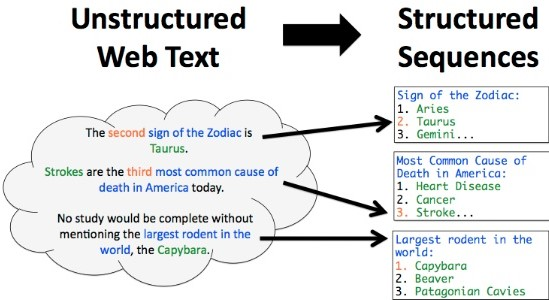
\includegraphics[width=\textwidth]{information-extraction}
		\caption[Information extraction example]{Information extraction, downloaded from\footnotemark}
	\end{figure}
\footnotetext{\url{https://www.slideshare.net/rubenizquierdobevia/information-extraction-45392844}}
%https://web.stanford.edu/~jurafsky/slp3/21.pdf


\subsection{Named Entity Recognition}\label{NER subsection}
Named Entity Recognition (NER) \cite{article:NER} is the problem of identifying and classifying proper names in text, including locations, such as China; people, such as George Bush; and organizations, such as the United Nations. The named-entity recognition task is, given a sentence, first to segment which words are part of entities, and then to classify each entity by type (person, organization, location, and so on). The challenge of this problem is that many named entities are too rare to appear even in a large training set, and therefore the system must identify them based only on context.

One approach to NER is to classify each word independently as one of either Person, Location, Organization, or Other (meaning not an entity). The problem with this approach is that it assumes that given the input, all of the named entity labels are independent. In fact, the named-entity labels of neighboring words are dependent; for example, while New York is a location, New York Times is an organization.

%The first step in most IE tasks is to find the proper names or named entities mentioned in a text. The task of named entity recognition (NER) is to find each mention of a named entity in the text and label its type. What constitutes a named entity type is application specific; these commonly include people, places, and organizations but also more specific entities from the names of genes and proteins(Cohen and Demner-Fushman, 2014) to the names of college courses (McCallum,2005).%[https://web.stanford.edu/~jurafsky/slp3/21.pdf]

%Named-entity recognition (NER) (also known as entity identification, entity chunking and entity extraction) is a subtask of information extraction (IE) that seeks to locate and classify named entities in text into pre-defined categories such as the names of persons, organizations, locations, expressions of times, quantities, monetary values, percentages, etc. \cite{wiki:NER}

Most research on NER systems has been structured as taking an unannotated block of text, such as this one:

Jim bought 300 shares of Acme Corp. in 2006.

And producing an annotated block of text that highlights the names of entities:

[Jim]Person bought 300 shares of [Acme Corp.]Organization in [2006]Time.

In this example, a person name consisting of one token, a two-token company name and a temporal expression have been detected and classified \cite{wiki:NER}.

	Figure~\ref{fig:StanfordNER} shows how one NER application can look like. The text in the example is predefined in Stanford NER application and loaded model (Classifier) is also trained by Stanford\footnote{https://nlp.stanford.edu/software/CRF-NER.html\#Models}.

	\begin{figure}[H]\centering
		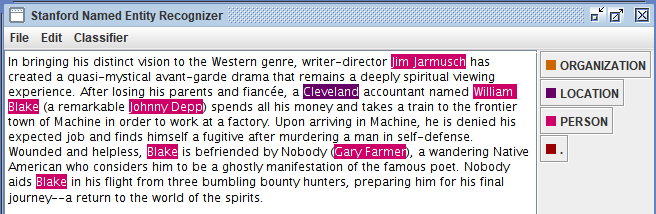
\includegraphics[width=\textwidth]{NER-Stanford}
		\caption{Stanford NER GUI with 3 classes model (Location, Person, Organization)}\label{fig:StanfordNER}
	\end{figure}

	There are several applications or frameworks for NER like Stanford NER, DBpedia Spotlight, spaCy, Chatbot NER, GATE, OpenNLP and so on. Here we will take a look only on the mentioned ones.

\subsubsection{Stanford NER}\label{Stanford NER}
Stanford NER\footnote{https://nlp.stanford.edu/software/CRF-NER.html} is a Java implementation of a Named Entity Recognizer. Named Entity Recognition (NER) labels sequences of words in a text which are the names of things, such as person and company names, or gene and protein names. It comes with well-engineered feature extractors for Named Entity Recognition, and many options for defining feature extractors. Included with the download are good named entity recognizers for English, particularly for the 3 classes (PERSON, ORGANIZATION, LOCATION), and we also make available on this page various other models for different languages and circumstances, including models trained on just the CoNLL 2003 English training data.

Stanford NER is also known as CRFClassifier. The software provides a general implementation of (arbitrary order) linear chain Conditional Random Field (CRF) sequence models. That is, by training your own models on labeled data, you can actually use this code to build sequence models for NER or any other task \cite{article:StanfordNER}.

\subsubsection{DBpedia Spotlight}\label{DBpedia Spotlight}
DBpedia Spotlight\footnote{https://www.dbpedia-spotlight.org/} \cite{wiki:DBpediaSpotlight} is a tool for annotating mentions of DBpedia resources in text. This allows linking unstructured information sources to the Linked Open Data cloud through DBpedia. DBpedia Spotlight performs named entity extraction, including entity detection and name resolution (in other words, disambiguation). It can also be used for named entity recognition, and other information extraction tasks. DBpedia Spotlight aims to be customizable for many use cases. Instead of focusing on a few entity types, the project strives to support the annotation of all 3.5 million entities and concepts from more than 320 classes in DBpedia. The project started in June 2010 at the Web Based Systems Group at the Free University of Berlin.

\subsubsection{spaCy}\label{spaCy}
spaCy\footnote{https://spacy.io/} \cite{wiki:spaCy} is an open-source software library for advanced Natural Language Processing, written in the programming languages Python and Cython. It offers the fastest syntactic parser in the world. The library is published under the MIT license and currently offers statistical neural network models for English, German, Spanish, Portuguese, French, Italian, Dutch and multi-language NER, as well as tokenization for various other languages.

\subsubsection{GATE}\label{GATE}
General Architecture for Text Engineering or GATE\footnote{https://gate.ac.uk/} \cite{wiki:GATE} is a Java suite of tools originally developed at the University of Sheffield beginning in 1995 and now used worldwide by a wide community of scientists, companies, teachers and students for many natural language processing tasks, including information extraction in many languages.

GATE includes an information extraction system called ANNIE (A Nearly-New Information Extraction System)\footnote{http://services.gate.ac.uk/annie/} which is a set of modules comprising a tokenizer, a gazetteer, a sentence splitter, a part of speech tagger, a named entities transducer and a coreference tagger. ANNIE can be used as-is to provide basic information extraction functionality, or provide a starting point for more specific tasks.

\subsubsection{OpenNLP}\label{OpenNLP}
The Apache OpenNLP library\footnote{http://opennlp.apache.org/docs/1.8.4/manual/opennlp.html\#intro.description} is a machine learning based toolkit for the processing of natural language text. It supports the most common NLP tasks, such as tokenization, sentence segmentation, part-of-speech tagging, named entity extraction, chunking, parsing, and coreference resolution. These tasks are usually required to build more advanced text processing services. OpenNLP also included maximum entropy and perceptron based machine learning.

The goal of the OpenNLP project will be to create a mature toolkit for the abovementioned tasks. An additional goal is to provide a large number of pre-built models for a variety of languages, as well as the annotated text resources that those models are derived from.

\subsubsection{Chatbot NER}\label{Chatbot NER}
Chatbot NER\footnote{https://haptik.ai/tech/open-sourcing-chatbot-ner/} is heuristic based that uses several NLP techniques to extract necessary entities from chat interface. In Chatbot, there are several entities that need to be identified and each entity has to be distinguished based on its type as a different entity has different detection logic. 



\subsection{RDF/NIF}
	The Resource Description Framework (RDF)\cite{wiki:RDF} is a family of World Wide Web Consortium (W3C) specifications originally designed as a metadata data model.  It is a framework for describing resources on the web; it is designed to be read and understood by computers.
	
	The information in RDF is represented by subject-predicate-object, known as triples. Triples are written in one of RDF notations: RDF/XML, RDFa, N-Triples, Turtle, JSON-LD and stored in a triplestore \cite{master:SPARQL}.
	
	RDF \cite{w3c:RDF} has features that facilitate data merging even if the underlying schemas differ, and it specifically supports the evolution of schemas over time without requiring all the data consumers to be changed.

	Natural Language Processing Interchange Format (NIF)\footnote{http://aksw.org/Projects/NIF.html} \cite{w3c:NIF} is an RDF-based format. The classes to represent linguistic data are defined in the NIF Core Ontology. All ontology classes are derived from the main class nif:String which respresents strings of Unicode characters.
	
%	\begin{lstlisting}[language=java]
%https://2018.eswc-conferences.org/wp-content/uploads/2018/02/ESWC2018_paper_136.pdf
%1 @ prefix rdf : <http :// www .w3.org /1999/02/22 - rdf - syntax -ns#> .
%2 @ prefix xsd : <http :// www .w3.org /2001/ XMLSchema #> .
%3 @ prefix itsrdf : <http :// www .w3. org /2005/11/ its / rdf #> .
%4 @ prefix nif : <> .
%5 @ prefix ex: <http :// nif . dbpedia . org/ wiki /en/> .
%6
%7 ex : United_States ? dbpv =2016 -10& nif = context
%8 a nif : Context ;
%9 nif : beginIndex "0"^^ xsd : nonNegativeInteger ;
%10 nif : endIndex " 104211 "^^ xsd : nonNegativeInteger ;
%11 nif : firstSection ex : United_States ? dbpv =2016 -10& char =0 ,4241 ;
%12 nif : lastSection ex : United_States ? dbpv =2016 -10& char =103211 ,104211 ;
%13 nif : hasSection ex : World_War_II ? dbpv =2016 -10& char =0 ,5001 ;
%14 nif : sourceUrl ex : United_States ? oldid =745182619 ;
%15 nif : predLang < http :// lexvo . org / id / iso639 -3/ eng > ;
%16 nif : isString " ... The first inhabitants of North America migrated from
%Siberia by way of the Bering land bridge ... " .
%17
%18 ex : United_States ? dbpv =2016 -10& char =7745 ,9418
%19 a nif : Section ;
%20 nif : beginIndex " 7745 "^^ xsd : nonNegativeInteger ;
%21 nif : endIndex " 9418 "^^ xsd : nonNegativeInteger ;
%22 nif : hasParagraph ex : United_States ? dbpv =2016 -10& char =7860 ,8740 ;
%23 nif : lastParagraph ex : United_States ? dbpv =2016 -10& char =8741 ,9418 ;
%24 nif : nextSection ex : United_States ? dbpv =2016 -10& char =9420 ,12898 ;
%25 nif : referenceContext ex : United_States ? dbpv =2016 -10& nif = context ;
%26 nif : superString ex : United_States ? dbpv =2016 -10& char =7548 ,7743 .
%27
%28 ex : United_States ? dbpv =2016 -10& nif = paragraph & char =7860 ,8740
%29 a nif : Paragraph ;
%30 nif : beginIndex " 7860 "^^ xsd : nonNegativeInteger ;
%31 nif : endIndex " 8740 "^^ xsd : nonNegativeInteger ;
%32 nif : nextParagraph ex : United_States ? dbpv =2016 -10& char =8741 ,9418 ;
%33 nif : referenceContext ex : United_States ? dbpv =2016 -10& nif = context ;
%34 nif : superString ex : United_States ? dbpv =2016 -10& char =7745 ,9418 .
%35
%36 ex : United_States ? dbpv =2016 -10& char =7913 ,7920
%37 a nif: Word ;
%38 nif : anchorOf " Siberia " ;
%39 nif : beginIndex " 7913 "^^ xsd : nonNegativeInteger ;
%40 nif : endIndex " 7920 "^^ xsd : nonNegativeInteger ;
%41 nif : referenceContext ex : United_States ? dbpv =2016 -10& nif = context ;
%42 nif : superString ex : United_States ? dbpv =2016 -10& char =7860 ,8740 ;
%43 itsrdf : taIdentRef < http :// dbpedia . org / resource / Siberia > .
%	\end{lstlisting}

\subsection{DBpedia}
DBpedia \cite{dbpedia:core} is a crowd-sourced community effort to extract structured content from the information created in various Wikimedia projects. This structured information resembles an open knowledge graph (OKG) which is available for everyone on the Web. A knowledge graph is a special kind of database which stores knowledge in a machine-readable form and provides a means for information to be collected, organised, shared, searched and utilised. Google uses a similar approach to create those knowledge cards during search.

	DBpedia data is served as Linked Data, which is revolutionizing the way applications interact with the Web. One can navigate this Web of facts with standard Web browsers, automated crawlers or pose complex queries with SQL-like query languages (e.g. SPARQL).

	At the time of writing this thesis the last version of DBpedia is 3.7.
\subsubsection{DBpedia NIF}\label{DBpediaNIF}
	DBpedia \cite{dbpedia:NIF} currently primarily focus on representing factual knowledge as contained in Wikipedia infoboxes. A vast amount of information, however, is contained in the unstructured Wikipedia article texts. In order to broaden and deepen the amount of structured DBpedia data, we are going a step further.

	With the representation of wiki pages in the NLP Interchange Format (NIF) we provide all information directly extractable from the HTML source code divided into three datasets:
	\begin{itemize}
		\item nif-context: the full text of a page as context (including begin and end index)
		\item nif-page-structure: the structure of the page in sections and paragraphs (titles, subsections etc.)
		\item nif-text-links: all in-text links to other DBpedia resources as well as external references
	\end{itemize}
	These datasets will serve as the groundwork for further NLP fact extraction tasks to enrich the gathered knowledge of DBpedia.

For the purposes of this thesis we will use DBpedia NIF dataset version 2016-04 (dbpv=2016-04).

\subsubsection{DBpedia ontology}\label{DBpediaOntology}
	The DBpedia Ontology is a shallow, cross-domain ontology, which has been manually created based on the most commonly used infoboxes within Wikipedia. The ontology currently covers 685 classes which form a subsumption hierarchy and are described by 2,795 different properties.

	Since the DBpedia 3.7 release, the ontology is a directed-acyclic graph, not a tree. Classes may have multiple superclasses, which was important for the mappings to schema.org. A taxonomy can still be constructed by ignoring all superclasses except the one that is specified first in the list and is considered the most important \cite{dbpedia:Ontology}. 

Dbpedia ontology classes can be found here \footnote{\url{http://mappings.dbpedia.org/server/ontology/classes/}}

The DBpedia Ontology currently contains about 4,233,000 instances. Figure~\ref{fig:Dbpedia-ontology} shows the number of instances for several classes within the ontology. [http://wiki.dbpedia.org/services-resources/ontology]

	\begin{figure}[H]\centering
		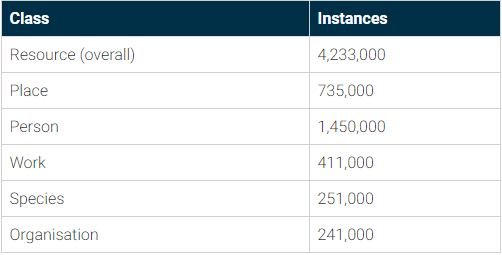
\includegraphics[width=\textwidth]{Dbpedia-ontology}
		\caption{Dbpedia Ontology - Instances per class}\label{fig:Dbpedia-ontology}
	\end{figure}

\subsection{Apache Jena}\label{ApacheJena}
	Apache Jena\footnote{\url{https://jena.apache.org/index.html}} \cite{wiki:ApacheJena} is an open source Semantic Web framework for Java. It provides an API to extract data from and write to RDF graphs. The graphs are represented as an abstract "model". A model can be sourced with data from files, databases, URLs or a combination of these. A Model can also be queried through SPARQL 1.1.

\subsection{SPARQL}\label{SPARQL}
	SPARQL \cite{master:SPARQL} is an RDF query language, that is, a semantic query language for databases, able to retrieve and manipulate data stored in Resource Description Framework (RDF) format. SPARQL works for any data source that can be mapped to RDF.

	SPARQL allows users to write queries against key-value data or, more specifically, data that can be mapped to RDF. The entire database is thus a set of subject-predicate-object triples.
	
	The SPARQL standard \footnote{\url{https://ontotext.com/knowledgehub/fundamentals/what-is-sparql/}} is designed and endorsed by the W3C and helps users and developers focus on what they would like to know instead of how a database is organized.

	In Listing~\ref{SPARQLexample} is an example of SPARQL query where we are selecting 10 abstracts from DBpedia NIF who has ontology type PoliticalParty and their PageRank and sort descending by PageRank.   
\begin{lstlisting}[caption=SPARQL example \label{SPARQLexample}]
PREFIX rdf:<http://www.w3.org/1999/02/22-rdf-syntax-ns#>
PREFIX dbo:<http://dbpedia.org/ontology/>
PREFIX vrank:<http://purl.org/voc/vrank#>

SELECT DISTINCT ?s ?v
FROM <http://dbpedia.org>
FROM <http://people.aifb.kit.edu/ath/#DBpedia_PageRank>
WHERE{
	?s rdf:type dbo:PoliticalParty .
	?s vrank:hasRank/vrank:rankValue ?v.
}
ORDER BY DESC(?v) LIMIT 10
\end{lstlisting}

\section{Related work}
In this section we will compare our approach and our chosen domains.
MISSING CONTENT!!!

\subsection{Domain specific Named Entity Recognition}
Traditionally Named Entity Recognition (NER)\cite{article:DomainSpecific} systems have been built using available annotated datasets (like CoNLL, MUC) and demonstrate excellent performance. However, these models fail to generalize onto other domains like Sports and Finance where conventions and language use can differ significantly. Furthermore, several domains do not have large amounts of annotated labeled data for training robust Named Entity Recognition models.
With specifying the domain we can create a bigger model with more annotated words and reading the whole text will be same or even faster that reading text with a global domain.  


%%%%%%%%%%%%%%%%%%%%%%%%%%%%%%%%%%%%%%%%%%%%%%%%%%%%%%%%%%%%%%%%%%%%%%%%%%%%%%%%%%%%%%%%%%%%%%
%%%%%%%%%%%%%%%%%%%%%%%%%%%%%NEW CHAPTER%%%%%%%%%%%%%%%%%%%%%%%%%%%%%%%%%%%%%%%%%%%%%%%%%%%%%%
%%%%%%%%%%%%%%%%%%%%%%%%%%%%%%CHAPTER 2%%%%%%%%%%%%%%%%%%%%%%%%%%%%%%%%%%%%%%%%%%%%%%%%%%%%%%%
\chapter{Domain specific named entity recognition}\label{}
	In this chapter we will go through the whole process of transforming raw DBpedia datasets to datasets that are ready for training a model with Stanford NER and how to train a model with Stanford NER. Section~\ref{dataPreProcessing} explains the process of cleaning the data from DBpedia NIF datasets and preparing them for processing. In Section~\ref{domainSpecification} we explain how we choose "POLITICS", "SPORT" and "TRANSPORTATION" domains. Section~\ref{typesRetrieval} shows all ontology types that we retrieve for every domain and grouping them to more specific ontology type. In Section~\ref{StanfordNERoutput} is explained the process of preparing datasets for training in Stanford NER. And finally in Section~\ref{modelGeneration} is shown how to train a datasets with Stanford NER.  

\section{Data pre-processing}\label{dataPreProcessing}
	To be able to create domain specific datasets ideally we need some big raw data. We choose data from DBpedia NIF Datasets (for more information about DBpedia NIF see Section~\ref{DBpediaNIF}) for the English language in .ttl format. From here we needed only 2 datasets, and that nif-context (or nif-abstract-context) and nif-text-links.

	Another dataset that we needed was DBpedia instance types dataset, found at DBpedia download page\footnote{\url{http://wiki.dbpedia.org/downloads-2016-04}} also in .ttl format. This dataset contains all types of nif-text-links that occurrence at nif-abstract-context file.

	So how all this dataset are connected between themselves? Let say that we have abstract for Alexander the Great. In nif-text-links file we have all words from the abstract that has annotation, but we still don't know their type. So here comes instance types file where based on link from nif-text-link (eg.http://dbpedia.org/resource/Philip\_II\_of\_Macedon) we can find the type of annotated word (word Philip II has ontology type Monarch), but of course, there can be a case that some words cannot be found on instance types file and automatically have no type, or in our case ontology type O (O stands for OTHER).

	But now, let us explain deeply how we process and clean data from the datasets. First, we define small test dataset to check how fast we can process data. Running that dataset on downloaded files without any cleaning on data takes too long. So we said that converting the datasets from RDF format to binary format (.ttl to .hdt) with RDF/HDT tool\footnote{\url{http://www.rdfhdt.org/}} will be faster. HDT (Header, Dictionary, Triples)\cite{FMPGPA:13} is a compact data structure and binary serialization format for RDF that keeps big datasets compressed to save space while maintaining search and browse operations without prior decompression. So we converted the datasets and reran the algorithm again. There were some improvements, but not satisfying for our purposes. Our next solution was to clean datasets from unused data for our aims. The final result after cleaning was a smaller datasets, for instance, nif-abstract-context file from 7.78GB now has 2.99GB, another big improvement was nif-text-links file who is reduced to 10.5GB from 44.6GB and at the end we also clean instance-types file, but here we don't record any mayor memory improvements. Again we rerun the algorithm, of course, there were improvements, but as well as previous the time that algorithm runs, was not acceptable for us. To give an illustration, the time needed to find all types from one abstract in a worst case, to read nif-text-links and instance type files until the end was around 3.5 minutes. Therefore once more we converted our cleaned datasets from RDF format(.ttl) to binary format(.hdt). And how in previous running there were again improvements, but those improvements don't fulfill our expectations. The final thing that we have to save us was creating a dataset tree only for nif-text-links and instance-types files. For nif-text-links file we created a tree where we have folders from "a-z", also special characters folders and other folder(this folder contains data that have a lower occurrence, let say \& character or letters that are not part of the English alphabet) and folders from "a-z" has subfolders also from "a-z". 

	To give a closer look how we create that tree, let say that we have an abstract for Volkswagen Golf MK3, so the link for that abstract would be http://dbpedia.org/resource/Volkswagen\_Golf\_Mk3 and this link will be stored to "v" folder and "o" subfolder, because the title of the abstract is Volkswagen Golf MK3, where we need only first 2 letters from the first word, in this case word Volkswagen. With this, we have a smaller dataset where we can read the whole one very fast.

	For instance types file we modified the algorithm for creating a data tree. Here because of lower range data we have created only files from "a-z", of course, special characters files and other file.

	Finally, we rerun the algorithm, and the time to process one abstract, at worst case, takes no longer than 1 minute. Now we were ready to take next steps to retrieve types (see Section~\ref{typesRetrieval}), create domains (see Section~\ref{domainSpecification}) and prepare data for Stanford NER (see Section~\ref{StanfordNERoutput}).

\section{Domain specification}\label{domainSpecification}
	As we said earlier most of the NER application are trained on same domains, like "PERSON", "ORGANIZATION" and "LOCATION". These 3 domains are widely spread all over the applications and perform nice results on text from this domains. So what we need is something that is not already trained or there is a small usage of that domain. After some research, we find out that "TRANSPORTATION" domain is not a popular domain for NER applications, respectively in time of writing the thesis we don't find any usage of this specific domain. So there is the possibility to create this specific domain. Types that we retrieve for this domain and groping them to more specific types are more deeply explained in Types retrieval (see Section~\ref{typesRetrieval}). We have our first domain, but at least 2 more domains are needed to be able to make some experiments and conclusion. 

	Ideally will be those domains to have some connection between them and again not to be already widespread. So we look at ontology types that are retrieved for "TRANSPORTATION" domain, and there are types like Airport, Bridge, MetroStation and so on. This indicates to us that next domain can be "POLITICS". Why? Because some airports, bridges or metro stations bear names of Politicians. For instance airport in Prague, Czech Republic is named by the last president of Czechoslovakia, Vaclav Havel. Or another example is that some bridges in the United States are named by famous politicians, like Presidents. The types that contains this domain are explained in Section~\ref{typesRetrieval}. The second domain is chosen, so we need at least one more domain to keep up with other NER applications. 
	
	With the requirements that we set for choosing a domain, which domain to choose was not easy at all. After a big research, also referring to ontology types from previous two domains and some NER applications (see Section~\ref{NER subsection}) we find an opportunity to create the last "SPORT" domain. Now we should check on DBpedia ontology classes page (see Section~\ref{DBpediaOntology}) how many ontology types we have for this domain. At the time of writing this thesis there were around 170 ontology types, which is very good number for creating a domain (for more see Section~\ref{typesRetrieval}).
	
After we complete choosing of domains, the next big think was to choose the right ontology types for every specific domain and if it is needed or make sense group those types to more specific type. This is totally covered and explained at Section~\ref{typesRetrieval}. 

\section{Types retrieval}\label{typesRetrieval}
	After we solved the problem of that how effectively run the algorithm to find all types from the abstract and choose domains, next issue was which types we want to be part of our domains and also which types we want to retrieve from Dbpedia. Worth mentioning that we will use the same ontology types for retrieving the abstracts links from Dbpedia and creating a domain models. For example the type "Politician" will be used to retrieve links from Dbpedia that has that type, and also "Politician" type will be use to annotated words, for instance Barack Obama will have type of "Politician" (we will give more details on section~\ref{StanfordNERoutput}).

	In DBpedia ontology classes page\footnote{\url{http://mappings.dbpedia.org/server/ontology/classes/}} we can see all types that DBpedia ontology has. Those ontology types are the same in instance types file also. Now we are facing with the fact that if we choose very small group of ontology types, at the experiment point we will have minor range of annotated words and experiments won't be relevant. On the other hand, if we go too deep to ontology types, we will have a lot of annotated words, which on one hand is good, but training the model will take a lot of time and memory, and there is a possibility that we will reach memory exception, or because of big group of types training will never end.  

After some testing with the number of retrieved types we finally found the best selection of types, in total we choose 283 ontology types for all domains.

Now let us explain more deeply every single domain and which types has that domain. We have 3 domains (see Section~\ref{domainSpecification} for that how we choose those domains) "POLITICS", "SPORT" and "TRANSPORTATION".

In "POLITICS" domain we retrieve in total 26 types, found at Appendix~\ref{PoliticsTypes}, which we sort in 11 more specific types like Ambassador, Chancellor, Congressman, Deputy, Governor, Lieutenant, Mayor, MemberOfParliament, Minister, President, PrimeMinister, Senator, VicePresident and VicePrimeMinister are joined together in one specific domain Politician, other types we leaved as it is, because if we group them the types wouldn't give any sense.  

	We do the same for "SPORT" domain where we retrieve in total 171 types, found in Appendix~\ref{SportTypes}, so those types, same as "POLITICS" domain, are more specified in 8 types, like SportClub, SportsLeague, SportsTeam, Athlete, Coach, OrganizationMember, SportsManager and SportsEvent. Grouping of types is also shown in appendix~\ref{SportTypes}. This domain is a nice example of that even we retrieve quite a big number of types, we can reduce that number with more specific types which further don't lose the sense of type. For instance "David de Gea" has a type of SoccerPlayer, but after processing will have type of Athlete, which gives sense, because any type of sport player is an athlete.

	At the end we repeat the process for "TRANSPORTATION" domain, where we retrieve in total 86 types. Retrieved types can be found in Appendix~\ref{TransportationTypes}. Those types are after minimized in 14 more specific types like Aircraft, Automobile, Locomotive, MilitaryVehicle, Motorcycle, On-SiteTransportation, Rocket, Ship, SpaceShuttle, SpaceStation, Spacecraft, Train, PublicTransitSystem and Infrastructure. The logic of that who we create more specific ontology types is same as in "POLITICS" or "SPORT" domain.   

	The reason why we group ontology types to more specific ones is that, that when the dataset has a smaller number of types, training a model with Stenford NER is more faster and requires less memory for training. Another reason is faster providing a NER, because is needed to read less types and also the overall results after testing with same data perform better than when ontology types where not grouped.

\section{Data transformation}\label{StanfordNERoutput}
	We define domains as well their types that we will retrieve and process, now we should put everything together and prepare data for Stanford NER application. In Data pre-processing (see Section~\ref{dataPreProcessing}) we explain how we handled the data downloaded from web and we briefly touch how those data will be prepared for training in Stanford NER application. 

	The final thing that is missing is how we will choose which abstracts will be part of our models. Because our goal is to create models with different number of abstracts we need some strict order of retrieved links from DBpedia dataset. The solution that we choose who fits to our requirements is PageRank. PageRank \cite{wiki:PR} is an algorithm used by Google Search to rank websites in their search engine results. So with a prepared and tested SPARQL queries on www.dbpedia.com/sparql and  with help of Apache Jena framework (see Section~\ref{ApacheJena}) we implemented retrieving links, on Java, on DBpedia endpoint\footnote{\url{http://www.dbpedia.com/sparql}}. After retrieving those data, based on their PageRank we search does retrieved link is part on our abstract file. If link is found in nif-abstract dataset it's written to two files, one file is where are written all abstracts from every domain and another file is file for that specific domain. Those files are creating in RDF format, with n-triples, that means that there is subject, in our case that is the link of abstract, then predicate who has isString annotation which tells that next triple contains the abstract text and finally object where abstract text is placed. Next thing that we need to do is to find all annotated words from abstract and their types. The algorithm of finding types is explained in Section~\ref{dataPreProcessing}. What is not mention there is that after finding the types, the abstract is written to file, where on first position is word and on the second position is the type of that word, if there is any, if not the type is O. Final step is to prepare data to be able to train models in Stanford NER with the types that we define in Section~\ref{typesRetrieval}. Because files contains all types that were found on the abstracts we need to clean and group them, as well to create a coarse and fine grained files. The algorithm is very simple, it reads the files who already has all types and if type is part of our retrieved types then either type is leaved as it is, or is grouped to more specific type, for instance if word has type Ambassador, then after filtering that word will have Politician type. The same is for coarse grained annotation, but here proper types after filtering are "POLITICS", "SPORT" or "TRANSPORTATION" type. The whole process is also illustrated at Algorithm~\ref{AlgorithmMain}.
		Interesting fact is that, that when we retrieve links from DBpedia with a specific ontology types types, some links there has types that are not even part of our domain. Here are some interesting links that we catch:
	
	\begin{itemize}
	\item http://dbpedia.org/page/Orbital\_period	
	\item http://dbpedia.org/page/Pregnancy
	\item http://dbpedia.org/page/Melody
	\item http://dbpedia.org/page/ITunes
	\item http://dbpedia.org/page/Tachycardia
	\item http://dbpedia.org/page/Shortwave\_radio
	\item http://dbpedia.org/resource/UTC-05:00
	\end{itemize}
	
	\begin{algorithm}
	Retrieve links from DBpedia NIF Dataset based on their PageRank\;
	\eIf{ Retrieved link is found at nif-abstract dataset}{
		write value from nif-abstract dataset to file
		}{
		go to next retrieved link and repeat steps		
		} 
	Read new file with values from nif-context and get abstract links\;
	Check does that link is consists in nif-text-links dataset\;
	\eIf{link consists in nif-text-links}{
		Get all values (links) from nif-text-links dataset\;
		Search for ontology types in instance-types dataset\;
		\eIf{Link from nif-text-links exists in instance-types}{
			Parse value and return ontology type\;		
		}

		Write abstract text to domain specific file with founded type of the word, as only word and the type at a line\;	
	}{
		Write abstract text to domain specific file with word and O type at a line\;  	
	}
	 
	Read created domain specific files and clean unnecessary types\;
	\eIf{Type equals some of retrieved types}{
		Leave type as it is or group type and write to two domain specific files in coarse and fine grained\; 	
	}{
		Rewrite the type to "O" and write to two domain specific files in coarse and fine grained\;
	}{
		Write to two domain specific files in coarse and fine grained\;	
	}
	\caption{Algorithm for preparing datasets ready for training in Stanford NER\label{AlgorithmMain}}
	\end{algorithm}
	
	   
	
\section{Model generation}\label{modelGeneration}
	With the created files from Section~\ref{StanfordNERoutput} now we can start training models. At Stanford NER CRF FAQ webpage\footnote{\url{https://nlp.stanford.edu/software/crf-faq.html}} is a very nice explanation of that how to train own model with Stanford NER. We follow those steps and used pretty much the same NER properties file with a small correction where we had to add 2 more flags to be able to train big models. Those two flags are saveFeatureIndexToDisk=true, which is used on every properties file and for creating a models in fine grained we use useObservedSequencesOnly=true.Flag saveFeatureIndexToDisk stands for saving the feature name's to disk that aren't actually needed while the core model estimation (optimization) code is run. More interesting is useObservedSequencesOnly flag. It's stands for labeling only adjacent words with label sequences that were seen next to each other in the training data. For some kinds of data this actually gives better accuracy, for other kinds it is worse. After testing on a small model with only 40 abstracts and model with 300 abstracts we find out that for creating a fine grained model with 40 and more abstract this flag gives us better results, while on coarse grained models this flag gives worst results, the exception are models with 500 abstracts where we should use this flag to reduce memory usage. The whole properties file with all used flags can be found in Appendix~\ref{NERpropertiesFile}.  
 
 After creating a properties files, training models is very easy with only one command, where unlike command from Stanford we add Xmx Java option, because standard command use only 4GB of RAM, which for our purposes is not enough for training big models. 
 
 Command for training model ran from the stanford-ner folder:
 \begin{lstlisting}{bash}
 	java -Xmx11g -cp stanford-ner.jar 
 	edu.stanford.nlp.ie.crf.CRFClassifier -prop 
 	locationAndnameOfPropFile.prop
 \end{lstlisting}
	
	\subsection{Training datasets}
	For the aim of our experiments we have trained 57 models. As mentioned earlier for training we have used Stanford NER application explained in Section~\ref{Stanford NER}. We have two types of models, coarse-grained and fine-grained, also those model types are divided in to "POLITICS", "SPORT" or "TRANSPORTATION" specific domains and a global domain who contains all abstracts from every domain. To give an illustration, for dataset with 100 retrieved abstract we will have 4 coarse-grained models (global domain and 3 specific domains), and similarly for a fine-grained models, so in total we have 8 trained models for every dataset. We created 7 different datasets with 10 abstracts, 20 abstracts, 40 abstracts, 100 abstracts, 300 abstracts, 400 abstracts and 500 abstracts. Each of this datasets has 8 trained models and we have one dataset that have also 500 abstracts, but those abstracts are not the same like the previous dataset. This dataset contains abstracts that have lower PageRank value and has only one trained model with abstracts from every domain in fine grained. 

 
%%%%%%%%%%%%%%%%%%%%%%%%%%%%%%%%%%%%%%%%%%%%%%%%%%%%%%%%%%%%%%%%%%%%%%%%%%%%%%%%%%%%%%%%%%%%
%%%%%%%%%%%%%%%%%%%%%%%%%%%%%NEW CHAPTER%%%%%%%%%%%%%%%%%%%%%%%%%%%%%%%%%%%%%%%%%%%%%%%%%%%%
%%%%%%%%%%%%%%%%%%%%%%%%%%%%%%CHAPTER 3%%%%%%%%%%%%%%%%%%%%%%%%%%%%%%%%%%%%%%%%%%%%%%%%%%%%%
\chapter{Experiments}

There are parameters of the computer used for tests shown in Table \ref{tab:PCparam}.
\begin{table}[H]\centering
	\caption{Testing computer parameters}
	\label{tab:PCparam}
	\begin{tabular}{|l|l|}
	\hline \multicolumn{1}{|c|}{\textbf{Part}} & \multicolumn{1}{|c|}{\textbf{Description}} \\\hline
	CPU & 2.00 GHz Intel(R) Core(TM) i5-4310U \\
	MEM & 16 GB DDR3L\\
	OS & x86\_64 Windows 10 Pro\\
	DISK & 240GB SSD Kingston\\\hline
	\end{tabular}
\end{table}


We have provide various types of experiments. In next sections we will discuss more about every provided experiment. The order of the abstracts is based on PageRank as explained in section~\ref{StanfordNERoutput}.

\section{Goals of the experiments}
	We set a few goals of the experiments. First of all we waned to test does we will get better results if we run the model of all domains in coarse grained, against the model of all domains in fine grained. In this test we run the models also with all domains texts. Then we get those models and we run it with specific domain texts, in both fine and coarse grained. Also we make experiments with specific domain model run with domain specific texts, for example, politics domain model in coarse grained is run with politics domain text also annotated in coarse grained, politics domain model in fine grained is run with politics domain text also annotated in fine grained, and the same for sport and transportation domains.

\section{Evaluation metrics}
	The success of NER systems is exposed to $F_{1}$ score (F-score or F-measure). $F_{1}$ \cite{wiki:F1} score  is a measure of a test's accuracy. It considers both the precision p  and the recall r of the test to compute the score: p is the number of correct positive results divided by the number of all positive results returned by the classifier, and r is the number of correct positive results divided by the number of all relevant samples (all samples that should have been identified as positive). The F1 score is the harmonic average of the precision and recall, where an F1 score reaches its best value at 1 (perfect precision and recall) and worst at 0. 
Written in formula, the $F_{1} =2\cdot \frac{precision \cdot recall}{precision + recall}$.


\section{List of experiments}
	With our trained models we made a few experiments. First one is the model that has 300 abstract on every domain(900 abstract in total). This is our main model and other experiments that we will provide like models that has lower or higher number of abstracts or experiments where model has more abstracts that a test file or vice-verse, all those results will be compared with the results obtained from main experiment. This experiment can be found an Section~\ref{MainExperiment}.
	With the experiments we wanted to answer some important questions, like:
\begin{itemize}
	\item Which is the impact on results when models are trained with less data than in the main experiment?
	
	To see the answer of this question, please referrer to Section~\ref{LessThan300Abstracts}.
	
	\item Which is the impact on results when models are trained with more data than in the main experiment? 
	
	Section~\ref{MoreThan300Abstracts} has answer to this question.
	
	\item What is the impact on results when models are train in fine or coarse grain? 
	
	In both sections (Section~\ref{LessThan300Abstracts} and Section~\ref{MoreThan300Abstracts} and as well in Section~\ref{MainExperiment} we provide those types of experiments.
	
	\item What is the impact on results when trained model is tested with more than one dataset? 
	
	Section~\ref{MixedExperiments} has the answer of this question.
	
	\item How the biggest train model will perform when is tested with texts from news papers?
	
	Section~\ref{NewsPapersEvaluation} gives a closer look to this question.

\end{itemize}



%
%Make it like experiment - discussion

%	\begin{figure}[H]\centering
%		\includegraphics[width=\textwidth]{"/500All3DomainsCoarseGrainedRunnedWithAll3DomainsBBCCoarseGrained-tsv".png}
%		\caption{All 3 Domains Coarse BBC Coarse}\label{}
%	\end{figure}
%	
%	\begin{table}[H]\centering
%		\caption{TABLE}
%		\label{}
%		\begin{tabular}{|l|c|r|l|}
%			\hline {\textbf{Entity}} & {\textbf{P}} & {\textbf{R}} & {\textbf{F1}}\\\hline
%				POLITICS & 0,9655 & 0,9333 & 0,9492\\
%				SPORT & 1,0000 & 1,0000 & 1,0000\\
%				TRANSPORTATION & 1,0000 & 1,0000 & 1,0000\\\hline
%				Totals & 0,9811 & 0,9630 & 0,9720\\\hline
%		\end{tabular}
%	\end{table}
\subsection{Main experiment}\label{MainExperiment}
	This is our main experiment where other experiments will be compared with this one. This model is trained with top 300 Wikipedia abstracts for every domain. Algorithm for preparing the data for training model explained in section~\ref{StanfordNERoutput}  takes 8622805705290 nanoseconds or 2.40 hours. The model is trained in coarse grained and takes 844.63 seconds in optimization and 873.7 seconds on CRFClassifier training.

\subsubsection{Global domain models}
	First experiment that we do with this model is that we run it with the same text that model is trained in coarse grained. Results are not bad at all, we are above 95\% as shown in Table~\ref{table:All3domainsWithAll3DomiansTop300Coarse}, which is great number for such middle weight model. With such results, someone will say that those are nice results and other experiments will only have a worst results. But let see how model will behaves when we tested with abstracts for every specific domain.

	\begin{table}[H]\centering
		\begin{tabular}{|l|l|l|l|}
			\hline {\textbf{Entity}} & {\textbf{P}} & {\textbf{R}} & {\textbf{F1}}\\\hline
				POLITICS & 0,9872 & 0,9462 & 0,9662\\
				SPORT & 0,9846 & 0,9629 & 0,9736\\
				TRANSPORTATION & 0,9940 & 0,9823 & 0,9881\\\hline
				\textbf{Totals} & \textbf{0,9875} & \textbf{0,9625} & \textbf{0,9748}\\\hline
		\end{tabular}
		\caption{Outcomes of base experiment run to be used as reference for subsequential experiments \label{table:All3domainsWithAll3DomiansTop300Coarse}}
	\end{table}	
	
	Table~\ref{table:All3domainsWithPoliticsTop300Coarse} shows the output of model when is tested with abstracts from a "POLITICS" domain. As we said in Section~\ref{StanfordNERoutput} this type of abstract has the biggest word annotation. Result is not even close with the result from previous experiment. Also, trained model annotated words with a "TRANSPORTATION" domain, where the test file don't have any word with that annotation. 
	
	\begin{table}[H]\centering
		\begin{tabular}{|l|l|l|l|}
			\hline {\textbf{Entity}} & {\textbf{P}} & {\textbf{R}} & {\textbf{F1}}\\\hline
				POLITICS & 0,9839 & 0,4025 & 0,5713\\
				TRANSPORTATION & 0,0000 & 1,0000 & 0,0000\\\hline
				\textbf{Totals} & \textbf{0,9792} & \textbf{0,4025} & \textbf{0,5705}\\\hline
		\end{tabular}
		\caption{Outcomes of base model in coarse grained run with "POLITICS" abstracts\label{table:All3domainsWithPoliticsTop300Coarse}}
	\end{table}	
	
	Table~\ref{table:All3domainsWithSportTop300Coarse} gives us results from abstracts from "SPORT" domain. Here we have the same results like in first experiment, but because trained model annotated some words with a "POLITICS" or "TRANSPORTATION", even those that our test file contains only abstracts from "SPORT" domains and words has only "SPORT" type, the overall result is only a little bit lower that the first experiment.

	\begin{table}[H]\centering
		\begin{tabular}{|l|l|l|l|}
			\hline {\textbf{Entity}} & {\textbf{P}} & {\textbf{R}} & {\textbf{F1}}\\\hline
				POLITICS & 0,0000 & 1,0000 & 0,0000\\
				SPORT & 0,9846 & 0,9628 & 0,9736\\
				TRANSPORTATION & 0,0000 & 1,0000 & 0,0000\\\hline
				\textbf{Totals} & \textbf{0,9819} & \textbf{0,9628} & \textbf{0,9722}\\\hline
		\end{tabular}
		\caption{Outcomes of base model in coarse grained run with "SPORT" abstracts \label{table:All3domainsWithSportTop300Coarse}}
	\end{table}	
	
	Table~\ref{table:All3domainsWithTransportationTop300Coarse} provide outcome with testing with abstracts only from "TRANSPORTATION" domain. As in the previous experiment, the result now is almost the same like in first experiment, but even thought that trained model, as in previous 2 experiments, annotated words with a "SPORT" type, the overall results is better that the experiment where test file contains all abstracts from every domain. 
	
	\begin{table}[H]\centering
		\begin{tabular}{|l|l|l|l|}
			\hline {\textbf{Entity}} & {\textbf{P}} & {\textbf{R}} & {\textbf{F1}}\\\hline
				SPORT & 0,0000 & 1,0000 & 0,0000\\
				TRANSPORTATION & 0,9940 & 0,9822 & 0,9880\\\hline
				\textbf{Totals} & \textbf{0,9861} & \textbf{0,9822} & \textbf{0,9841}\\\hline
		\end{tabular}
	\caption{Outcomes of base model in coarse grained run with "TRANSPORTATION" abstracts \label{table:All3domainsWithTransportationTop300Coarse}}
	\end{table}	
	
	In conclusion with this kind of experiments we can say that it is not a good idea to train a model with all chosen domains and then use texts from specific domain to perform NER.
%%%%%%%%%%%%%%%%%%%%%%%%%%%%%%%%%%%%%%%%%%%%%%%%%%%%%%%%%%%%%%%%%%%%%%%%%%%%%%%%
	
	After we finish the experiments with model that is trained with all abstracts from every domain in coarse grained, we waned to see the impact of model that is trained with same abstracts, but now annotated in fine grained. To train this model we needed 3250.9 seconds from which 3207.45 seconds for optimization. Table~\ref{table:All3domainsWithAll3DomainsTop300Fine} shows the results of provided experiment where we can see that we have a little bit more better total result than experiment in Table~\ref{table:All3domainsWithAll3DomiansTop300Coarse}.


\begin{table}[H]\centering
		\begin{tabular}{|l|l|l|l|}
			\hline {\textbf{Entity}} & {\textbf{P}} & {\textbf{R}} & {\textbf{F1}}\\\hline
				Aircraft & 1,0000 & 1,0000 & 1,0000\\
				Athlete & 1,0000 & 0,9802 & 0,9900\\
				Automobile & 1,0000 & 1,0000 & 1,0000\\ 
				Coach & 1,0000 & 1,0000 & 1,0000\\
				Infrastructure & 1,0000 & 0,9820 & 0,9909\\
				PoliticalParty & 0,9860 & 0,9628 & 0,9743\\
				Politician & 1,0000 & 0,9353 & 0,9665\\
				PublicTransitSystem & 0,9919 & 0,9839 & 0,9879\\
				Ship & 1,0000 & 1,0000 & 1,0000\\
				SpaceShuttle & 1,0000 & 1,0000 & 1,0000\\
				SpaceStation & 1,0000 & 1,0000 & 1,0000\\ 
				SportsClub & 0,9796 & 0,9683 & 0,9739\\
				SportsEvent & 1,0000 & 0,9242 & 0,9606\\
				SportsLeague & 0,9647 & 0,9805 & 0,9725\\
				SportsManager & 1,0000 & 0,9423 & 0,9703\\
				SportsTeam & 1,0000 & 0,9805 & 0,9902\\
				Train & 1,0000 & 1,0000 & 1,0000\\\hline
				\textbf{Totals} & \textbf{0,9880} & \textbf{0,9712} & \textbf{0,9795}\\\hline
		\end{tabular}
		\caption{Outcomes of base experiment in fine grained run to be used as reference for subsequential experiments \label{table:All3domainsWithAll3DomainsTop300Fine}}
	\end{table}

Then we tested our model with abstracts from "POLITICS" domain. How we can see from Table~\ref{table:All3domainsWithPoliticsTop300Fine} there is some improvements on overall result unlike the experiment in coarse grained, but no satisfying at all. As well table shows that some words again are annotated with types from "SPORT" and "TRANSPORTATION" domain.

	\begin{table}[H]\centering
		\begin{tabular}{|l|l|l|l|}
			\hline {\textbf{Entity}} & {\textbf{P}} & {\textbf{R}} & {\textbf{F1}}\\\hline
				Election & 0,0000 & 0,0000 & 0,0000\\
				PoliticalParty & 0,9860 & 0,9628 & 0,9743\\
				Politician & 1,0000 & 0,1849 & 0,3120\\
				PublicTransitSystem & 0,0000 & 1,0000 & 0,0000\\
				Ship & 0,0000 & 1,0000 & 0,0000\\
				SportsLeague & 0,0000 & 1,0000 & 0,0000\\\hline
				\textbf{Totals} & \textbf{0,9825} & \textbf{0,4072} & \textbf{0,5758}\\\hline
		\end{tabular}
		\caption{Outcomes of base model in fine grained run with "POLITICS" abstracts\label{table:All3domainsWithPoliticsTop300Fine}}
	\end{table}	

    After that we rerun the experiment, but now with abstracts from "SPORT" domain. In Table~\ref{table:All3domainsWithSportTop300Fine} we can see minor growth of the results unlike experiment in Table~\ref{table:All3domainsWithSportTop300Coarse}, but this improvements are so small that are almost unimportant. Also our model annotated some words with types from "POLITICS" and "TRANSPORTATION" domain which the test file don't have those types at all.
    
	\begin{table}[H]\centering
		\begin{tabular}{|l|l|l|l|}
			\hline {\textbf{Entity}} & {\textbf{P}} & {\textbf{R}} & {\textbf{F1}}\\\hline
				Athlete & 1,0000 & 0,9802 & 0,9900\\
				Coach & 1,0000 & 1,0000 & 1,0000\\
				Politician & 0,0000 & 1,0000 & 0,0000\\
				SportsClub & 0,9794 & 0,9680 & 0,9737\\
				SportsEvent & 1,0000 & 0,9242 & 0,9606\\
				SportsLeague & 0,9678 & 0,9805 & 0,9741\\
				SportsManager & 1,0000 & 0,9423 & 0,9703\\				
				SportsTeam & 1,0000 & 0,9804 & 0,9901\\
				Train & 0,0000 & 1,0000 & 0,0000\\\hline
				\textbf{Totals} & \textbf{0,9821} & \textbf{0,9716} & \textbf{0,9768}\\\hline
		\end{tabular}
		\caption{Outcomes of base model in fine grained run with "SPORT" abstracts \label{table:All3domainsWithSportTop300Fine}}
	\end{table}
	
    Finally the last experiment with this model are the abstracts from "TRANSPORTATION" domain. Table~\ref{table:All3domainsWithTransportationTop300Fine} shows the output of the provided experiment, where like in previous 2 experiments we can notice a very little improvements on results, from experiment in Table~\ref{table:All3domainsWithTransportationTop300Coarse}, who again can be unimportant. As in previous experiments similarly here model annotated some words with types from other 2 domains, which test file does not even contains.

	\begin{table}[H]\centering
		\begin{tabular}{|l|l|l|l|}
			\hline {\textbf{Entity}} & {\textbf{P}} & {\textbf{R}} & {\textbf{F1}}\\\hline
				Aircraft & 1,0000 & 1,0000 & 1,0000\\
				Automobile & 1,0000 & 1,0000 & 1,0000\\				
				Infrastructure & 1,0000 & 0,9820 & 0,9909\\
				Politician & 0,0000 & 1,0000 & 0,0000\\				
				PublicTransitSystem & 0,9918 & 0,9837 & 0,9878\\
				Ship & 1,0000 & 1,0000 & 1,0000\\				
				SpaceShuttle & 1,0000 & 1,0000 & 1,0000\\
				SpaceStation & 1,0000 & 1,0000 & 1,0000\\
				SportsClub & 0,0000 & 1,0000 & 0,0000\\
				SportsTeam & 0,0000 & 1,0000 & 0,0000\\
				Train & 1,0000 & 1,0000 & 1,0000\\\hline
				\textbf{Totals} & \textbf{0,9862} & \textbf{0,9881} & \textbf{0,9871}\\\hline
		\end{tabular}
		\caption{Outcomes of base model in fine grained run with "TRANSPORTATION" abstracts\label{table:All3domainsWithTransportationTop300Fine}}
	\end{table}	
	
	Provided experiments with the model who is trained with all abstracts from every domain annotated in fine grained, overall provide a very little improvement on results on every experiment. With that observation trained model annotated in fine grained is better to use instead of the model that is annotated in coarse grained. Another benefit of this type of model is that we can see which types are annotated and their results. But, because those improvements are small and is needed almost four times more time to train a fine grained model, maybe the better solution will be a models trained in coarse grained, everything depends on us. Does we want to trained models faster or we want to be more precise. 

%%%%%%%%%%%%%%%%%%%%%%%%%%%%%%%%%%%%%%%%%%%%%%%%%%%%%%%%%%%%%%%%%%%%%%%%%%%%%%%%%%%%%%%%%%%%%%%%%%%%%%
\subsubsection{Evaluation of domain specific models}

	After completing experiments with a global domains in coarse and fine grained, now we will make experiments with models for specific domains.
	
	To train "POLITICS" domain specific model we need 66.7 seconds in total from which 59.53 seconds spend on optimization. In Table~\ref{table:PoliticsdomainsWithPoliticsTop300Coarse} the experiment is provided with model trained only with abstracts from "POLITICS" domain and run with the same texts that model in trained, in coarse grained. The result here is better than experiment in Table~\ref{table:All3domainsWithPoliticsTop300Coarse}, but worse that experiment provided with global domain in Table~\ref{table:All3domainsWithAll3DomiansTop300Coarse}. This can be cause by the fact that model has  biggest number of annotated words.

	\begin{table}[H]\centering
		\begin{tabular}{|l|l|l|l|}
			\hline {\textbf{Entity}} & {\textbf{P}} & {\textbf{R}} & {\textbf{F1}}\\\hline
				POLITICS & 0,8039 & 0,6779 & 0,7355\\\hline
				\textbf{Totals} & \textbf{0,8039} & \textbf{0,6779} & \textbf{0,7355}\\\hline
		\end{tabular}
		\caption{Outcomes of "POLITICS" base model in coarse grained run with "POLITICS" abstracts \label{table:PoliticsdomainsWithPoliticsTop300Coarse}}
	\end{table}
	
	We repeat previous experiment, but now everything in fine grained. Time for training this kind of model i total was 163.5 seconds, from which 155.94 seconds spend on optimization. Table~\ref{table:PoliticsdomainsWithPoliticsTop300Fine} shows that this kind of model provides better result that coarse grained model and the experiment provided in Table~\ref{table:All3domainsWithPoliticsTop300Fine}, but again worst than model trained with all abstracts (see Table~\ref{table:All3domainsWithAll3DomainsTop300Fine}).
	 
	\begin{table}[H]\centering
		\begin{tabular}{|l|l|l|l|}
			\hline {\textbf{Entity}} & {\textbf{P}} & {\textbf{R}} & {\textbf{F1}}\\\hline
				Election & 0,8240 & 0,6398 & 0,7203\\
				PoliticalParty & 0,8100 & 0,7006 & 0,7513\\
				Politician & 0,8599 & 0,7234 & 0,7858\\\hline
				\textbf{Totals} & \textbf{0,8354} & \textbf{0,6980} & \textbf{0,7606}\\\hline
		\end{tabular}
		\caption{Outcomes of "POLITICS" base model in fine grained run with "POLITICS" abstracts \label{table:PoliticsdomainsWithPoliticsTop300Fine}}
	\end{table}	
	
	In conclusion with provided 2 experiments and from this point of view, for this domain we can say that training a specific model will give better results and will perform faster that global domain tested with text from specific domain. On the other hand the global domain tested with a texts that is trained, how we can see from Table~\ref{table:All3domainsWithAll3DomainsTop300Fine} and Table~\ref{table:All3domainsWithAll3DomiansTop300Coarse} perform even better results that specific trained models.  
%%%%%%%%%%%%%%%%%%%%%%%%%%%%%%%%%%%%%%%%%%%%%%%%%%%%%%%%%%%%%%%%%%%%%%%%%%%%%%%%%%%%%%%%%%%%%%%%%%%%%%%%%%%%%


Next experiment that we do is the same like the previous one, but now the domain is "SPORT". Training time for this model was 93.0 seconds in total, but 82.97 seconds spend on optimization. This model and test file, how in previous one is run with 300 abstracts. Table~\ref{table:SportdomainsWithSportTop300Coarse} shows the outcome of the experiment in coarse grained. From the table we can see that this domain provide a better result that "POLITICS" domain, because here we have less annotated words. But, when compared with base experiment from Table~\ref{table:All3domainsWithAll3DomiansTop300Coarse} and Table~\ref{table:All3domainsWithSportTop300Coarse} those experiments perform better results that this one. 
	\begin{table}[H]\centering
		\begin{tabular}{|l|l|l|l|}
			\hline {\textbf{Entity}} & {\textbf{P}} & {\textbf{R}} & {\textbf{F1}}\\\hline
				SPORT & 0,9432 & 0,8839 & 0,9126\\\hline
				\textbf{Totals} & \textbf{0,9432} & \textbf{0,8839} & \textbf{0,9126}\\\hline
		\end{tabular}
		\caption{Outcomes of "SPORT" base model in coarse grained run with "SPORT" abstracts \label{table:SportdomainsWithSportTop300Coarse}}
	\end{table}

Also we train a model in fine grained, with total time of 554.9 seconds, with 543.55 seconds spend on optimization and provide an experiment. Table~\ref{table:SportdomainsWithSportTop300Fine} show that the result is little bit more better that result with model in coarse grained, but still this result is lower that the results for Table~\ref{table:All3domainsWithAll3DomainsTop300Fine} and Table~\ref{table:All3domainsWithSportTop300Fine}.
	\begin{table}[H]\centering
		\begin{tabular}{|l|l|l|l|}
			\hline {\textbf{Entity}} & {\textbf{P}} & {\textbf{R}} & {\textbf{F1}}\\\hline
				Athlete & 0,9713 & 0,8366 & 0,8989\\
				Coach & 1,0000 & 0,7500 & 0,8571\\
				SportsClub & 0,9453 & 0,9041 & 0,9242\\
				SportsEvent & 1,0000 & 0,7879 & 0,8814\\
				SportsLeague & 0,9418 & 0,8958 & 0,9182\\
				SportsManager & 1,0000 & 0,9615 & 0,9804\\				
				SportsTeam & 0,9845 & 0,8301 & 0,9007\\\hline
				\textbf{Totals} & \textbf{0,9592} & \textbf{0,8750} & \textbf{0,9152}\\\hline
		\end{tabular}
		\caption{Outcomes of "SPORT" base model in fine grained run with "SPORT" abstracts \label{table:SportdomainsWithSportTop300Fine}}
	\end{table}
	
	After provided 2 experiments with trained models for specific domain, the results shows that training a global model will perform better result than training a domain specific model.	
%%%%%%%%%%%%%%%%%%%%%%%%%%%%%%%%%%%%%%%%%%%%%%%%%%%%%%%%%%%%%%%%%%%%%%%%%%%%%%%%%%%%%%%%%%%%%%%%%

Final experiment that we do with this size of abstracts (300 abstracts) is with "TRANSPORTATION" domain. We needed 58.9 seconds to train the model, from which 50.35 seconds on optimization.
  Table~\ref{table:TransportationDomainsWithTransportationTop300Coarse} show the experiment outcome in coarse grained, where we can see that this result is lower than results from experiments provided in Table~\ref{table:All3domainsWithAll3DomiansTop300Coarse} and Table~\ref{table:All3domainsWithTransportationTop300Coarse}.  
	\begin{table}[H]\centering
		\begin{tabular}{|l|l|l|l|}
			\hline {\textbf{Entity}} & {\textbf{P}} & {\textbf{R}} & {\textbf{F1}}\\\hline
				TRANSPORTATION & 0,9583 & 0,9109 & 0,9340\\\hline
				\textbf{Totals} & \textbf{0,9583} & \textbf{0,9109} & \textbf{0,9340}\\\hline
		\end{tabular}
		\caption{Outcomes of "TRANSPORTATION" base model in coarse grained run with "TRANSPORTATION" abstracts \label{table:TransportationDomainsWithTransportationTop300Coarse}}
	\end{table}
	
	Finally we make an experiment in fine grained. Total training time was 702.6 seconds, from which 686.50 seconds spend on optimization. In Table~\ref{table:TransportationDomainsWithTransportationTop300Fine} we can see the results of provided experiment, where those results are even worse that the experiment with coarse grained model, which in previous two domain, "SPORT" and "POLITICS" was not that case. Also those results are worse than the experiments with a global domain in Table~\ref{table:All3domainsWithAll3DomainsTop300Fine} and Table~\ref{table:All3domainsWithTransportationTop300Fine}. 
	\begin{table}[H]\centering
		\begin{tabular}{|l|l|l|l|}
			\hline {\textbf{Entity}} & {\textbf{P}} & {\textbf{R}} & {\textbf{F1}}\\\hline
				Aircraft & 0,9659 & 0,8333 & 0,8947\\
				Automobile & 1,0000 & 0,8000 & 0,8889\\				
				Infrastructure & 0,9550 & 0,9550 & 0,9550\\
				PublicTransitSystem & 0,9662 & 0,9309 & 0,9482\\
				Ship & 1,0000 & 0,6429 & 0,7826\\				
				SpaceShuttle & 1,0000 & 0,8333 & 0,9091\\
				SpaceStation & 0,0000 & 1,0000 & 0,0000\\
				Train & 1,0000 & 1,0000 & 1,0000\\\hline
				\textbf{Totals} & \textbf{0,9660} & \textbf{0,9010} & \textbf{0,9324}\\\hline
		\end{tabular}
		\caption{Outcomes of "TRANSPORTATION" base model in fine grained run with "TRANSPORTATION" abstracts \label{table:TransportationDomainsWithTransportationTop300Fine}}
	\end{table}	

	In conclusion with the provided experiments in this section, we can say that training a global model and providing a NER is a better, but a little bit slowest solution than training a domain specific model, except the "POLITICS" domain, where the results was better in domain specific model unlike the experiment with a global domain and test file with "POLITICS" abstracts, but worse than experiment with a global domain tested with abstracts from all 3 domains. Then we waned to see the impact of fine grained trained models, where in most of the cases this kind of models provide a better results than models trained in coarse grained, except the experiment in "TRANSPORTATION" specific domain where the coarse grained model was better that fine grained model.
	
	After we finish with the main experiment, we were interested about the impact of the size of abstracts that will be used for training models. Next two subsections show the behavior of trained models.     
%%%%%%%%%%%%%%%%%%%%%%%%%%%%%%%%%%%%%%%%%%%%%%%%%%%%%%%%%%%%%%%%%%%%%%%%%%%%%%%%%%%%%%%%%%%%%%%%%%%%%%%%%%%%%%%%%%%%%%%%%%%%%%%%%%%%%%%%%%%%%%%%%%%%%%%%%%%%%%%%%%%%%%%%%%%%%%%%%%%%%%%%%%%%%%%%%%%%%%%%%%%%%%%%%%%%%%%%%%%%%%%%%%%%%%%%%%%%%%%%%%%%%%%%%%%%%%%%%%%%%%%%%%%%%%%%%%%%%%%%%%%%%%%%%%%%%%%%%%%%%%%%%%%%%%%%%%%%%%
\subsection{Experiments that has less than 300 abstracts in model}\label{LessThan300Abstracts}
	In this subsection we want to see the behavior of models that are trained with less than 300 abstracts. First experiment is trained with 10 abstracts, then we have experiments with 20 abstracts, next experiment with 40 abstracts, and finally experiment with 100 abstracts. The order of abstracts, how we said earlier, is based on PageRank.
	
	\textbf{Model trained with 10 abstracts to every domain.} To retrieve links from DBpedia with SPARQL and prepare data to be able to train models with 10 abstract, our algorithm explain in Section~\ref{StanfordNERoutput} takes in total 10.81 minutes, which comparing with main experiment, where we need 2.40 hours, is way more faster to prepare data. Of coarse this indicates that training models will also be faster than in main experiment.
	
	\textbf{Coarse grained model.} 
	\textbf{Description of the experiment.} How in the main experiment, also here we start with model trained in coarse grained. To train this kind of model we need 19.6 seconds, from which 17.44 seconds spend on optimization. 
	
	\textbf{Results of the experiment.} From Table~\ref{table:GlobalDomainWithAllAbstractsTop10Coarse} we see that trained model perform the best results without any loosing of words in "SPORT" and "TRANSPORTATION" domains, but worst result in "POLITICS" domain. The result of "POLITICS" domain is even worst than the result from main experiment provided in Table~\ref{table:All3domainsWithAll3DomiansTop300Coarse}. Because of this, there is a little bit lower overall result than in the main experiment. This can indicates that training models with lowest number of abstracts, for this kind of domains, is not worth. But let's see how model will behaves when is tested with abstracts from a specific domains.
	
	\begin{table}[H]\centering
		\begin{tabular}{|l|l|l|l|}
			\hline {\textbf{Entity}} & {\textbf{P}} & {\textbf{R}} & {\textbf{F1}}\\\hline
				POLITICS & 0,9655 & 0,9333 & 0,9492\\
				SPORT & 1,0000 & 1,0000 & 1,0000\\
				TRANSPORTATION & 1,0000 & 1,0000 & 1,0000\\\hline
				\textbf{Totals} & \textbf{0,9811} & \textbf{0,9630} & \textbf{0,9720}\\\hline
		\end{tabular}
	\caption{Outcomes of global model in coarse grained run with 10 abstracts from every domain \label{table:GlobalDomainWithAllAbstractsTop10Coarse}}
	\end{table}

	\textbf{Description of the experiment.} In this experiment we take the same model from the previous one, but now tested only with dataset that contains abstracts from "POLITICS" domain.
	
	\textbf{Results of the experiment.} Table~\ref{table:GlobalDomainWithPoliticsTop10Coarse} show the output of experiment where we have global model that is tested with 10 abstracts from "POLITICS" domain. Here model do not annotated any word from other domains unlike in the main experiment in Table~\ref{table:All3domainsWithPoliticsTop300Coarse}, but even this and the fact that here are much less abstracts does not help to provide a better results.
	
	\begin{table}[H]\centering
		\begin{tabular}{|l|l|l|l|}
			\hline {\textbf{Entity}} & {\textbf{P}} & {\textbf{R}} & {\textbf{F1}}\\\hline
				POLITICS & 0,9655 & 0,3636 & 0,5283\\\hline
				%SPORT & 1,0000 & 1,0000 & 1,0000\\\hline
				%TRANSPORTATION & 1,0000 & 1,0000 & 1,0000\\\hline
				\textbf{Totals} & \textbf{0,9655} & \textbf{0,3636} & \textbf{0,5283}\\\hline
		\end{tabular}
		\caption{Outcomes of global model in coarse grained run with 10 abstracts from "POLITICS" domain \label{table:GlobalDomainWithPoliticsTop10Coarse}}
	\end{table}

	\textbf{Description of the experiment.} For purposes of this experiment we have again used global model, but now tested with abstracts only from "SPORT" domain. 
	
	\textbf{Results of the experiment.} Table~\ref{table:GlobalDomainWithSportTop10Coarse} show the outcome of the experiment. We can see that model perform perfect result, how in experiment in Table~\ref{table:GlobalDomainWithAllAbstractsTop10Coarse} without any misleading annotations, which we cannot say for the main experiment where model annotated words from "POLITICS" and "TRANSPORTATION" domains. 
	
	\begin{table}[H]\centering
		\begin{tabular}{|l|l|l|l|}
			\hline {\textbf{Entity}} & {\textbf{P}} & {\textbf{R}} & {\textbf{F1}}\\\hline
				SPORT & 1,0000 & 1,0000 & 1,0000\\\hline
				\textbf{Totals} & \textbf{1,0000} & \textbf{1,0000} & \textbf{1,0000}\\\hline
		\end{tabular}
		\caption{Outcomes of global model in coarse grained run with 10 abstracts from "SPORT" domain \label{table:GlobalDomainWithSportTop10Coarse}}	
	\end{table}	

	\textbf{Description of the result.} Finally we tested the model with abstract from "TRANSPORTATION" domain. 
	
	\textbf{Results of the experiment.} From Table~\ref{table:GlobalDomainWithTransportationTop10Coarse} we can see that model as well as in previous experiment perform maximum result without misleading annotations, unlike the main experiment where how we can see from Table~\ref{table:All3domainsWithTransportationTop300Coarse} model annotate words with "SPORT" domain and has a lowest result than this one.
	
	\begin{table}[H]\centering
		\begin{tabular}{|l|l|l|l|}
			\hline {\textbf{Entity}} & {\textbf{P}} & {\textbf{R}} & {\textbf{F1}}\\\hline
				TRANSPORTATION & 1,0000 & 1,0000 & 1,0000\\\hline
				\textbf{Totals} & \textbf{1,0000} & \textbf{1,0000} & \textbf{1,0000}\\\hline
		\end{tabular}
		\caption{Outcomes of global model in coarse grained run with 10 abstracts from "TRANSPORTATION" domain \label{table:GlobalDomainWithTransportationTop10Coarse}}	
	\end{table}

	In conclusion with the results from provided experiments we see that there is a huge impact of the number of abstracts for training a global model in coarse grained. We see that for "SPORT" and "TRANSPORTATION" domain our model provide maximum results, which is what we want to reach.

%%%%%%%%%%%%%%%%%%%%%%%%%%%%%%%%%%%%%%%%%%%%%%%%%%%%%%%%%%%%%%%%%%%%%%%%%%%%%%%%%%%%%%%%%%%%%%	

	\textbf{Fine grained model.} After we finish the experiments with global models in coarse grained, we waned to see the impact of fine grained model. Does also here this kind of model will perform better results as was the case in main experiment, where global fine grained model perform a slide better results.
	
	\textbf{Description of the experiment.} Training a fine grained model takes in total 124.7 seconds, from which 120,73 seconds spent in optimization. In this experiment, the model is tested with the same dataset that is trained.
	
	\textbf{Results of the experiment.}From Table~\ref{table:GlobalDomainWithAllAbstractsTop10Fine} we can see that now fine grained model provide exactly the same overall result as well as coarse grained model. Also from table we can see in which ontology type our model fails to perform maximum result. So, because of PoliticalParty type where we have a lowest result, the total result is not at the maximum level, even thought other ontology types has maximum annotation.
	  	
	\begin{table}[H]\centering
		\begin{tabular}{|l|l|l|l|}
			\hline {\textbf{Entity}} & {\textbf{P}} & {\textbf{R}} & {\textbf{F1}}\\\hline
				Aircraft & 1,0000 & 1,0000 & 1,0000\\
				Athlete & 1,0000 & 1,0000 & 1,0000\\
				Coach & 1,0000 & 1,0000 & 1,0000\\
				PoliticalParty & 0,9600 & 0,9231 & 0,9412\\
				Politician & 1,0000 & 1,0000 & 1,0000\\
				PublicTransitSystem & 1,0000 & 1,0000 & 1,0000\\
				Ship & 1,0000 & 1,0000 & 1,0000\\
				SportsClub & 1,0000 & 1,0000 & 1,0000\\
				SportsEvent & 1,0000 & 1,0000 & 1,0000\\
				SportsLeague & 1,0000 & 1,0000 & 1,0000\\
				SportsTeam & 1,0000 & 1,0000 & 1,0000\\\hline
				\textbf{Totals} & \textbf{0,9811} & \textbf{0,9630} & \textbf{0,9720}\\\hline
		\end{tabular}
		\caption{Outcomes of global model in fine grained run with 10 abstracts from every domain \label{table:GlobalDomainWithAllAbstractsTop10Fine}}	
	\end{table}

	\textbf{Description of the experiment.} Then how in previous experiments, we take the global train model and test it with abstracts from every specific domain separately. 
	
	\textbf{Results of the experiment.} The first domain abstracts was from "POLITICS" domain, where from Table~\ref{table:GlobalDomainWithPoliticsTop10Fine} we can see that model perform same result as well as in coarse grained model experiment in Table~\ref{table:GlobalDomainWithPoliticsTop10Coarse}. Also even our model and test files has words with Election ontology type, the model do not recognize any of them. With that misleading we have lower results, if that doesn't happens the model will perform pretty mach good recognition.
	
	\begin{table}[H]\centering
		\begin{tabular}{|l|l|l|l|}
			\hline {\textbf{Entity}} & {\textbf{P}} & {\textbf{R}} & {\textbf{F1}}\\\hline
				Election & 0,0000 & 0,0000 & 0,0000\\
				PoliticalParty & 0,9600 & 0,9231 & 0,9412\\
				Politician & 1,0000 & 1,0000 & 1,0000\\\hline
				\textbf{Totals} & \textbf{0,9655} & \textbf{0,3636} & \textbf{0,5283}\\\hline
		\end{tabular}
		\caption{Outcomes of global model in fine grained run with 10 abstracts from "POLITICS" domain \label{table:GlobalDomainWithPoliticsTop10Fine}}		
	\end{table}	

	\textbf{Description of the experiment.} In this experiment we also used the global model, but now tested with dataset that contains only abstracts from "SPORT" domain. 
	
	\textbf{Results of the experiment.}Table~\ref{table:GlobalDomainWithSportTop10Fine} shows that our model recognize all annotated words from test file without any misleading and perform maximum F1 score. In comparing with the main experiment in Table~\ref{table:All3domainsWithSportTop300Fine} where we have some loosing, here that is not the case and it is what we want to reach.
	
	\begin{table}[H]\centering
		\begin{tabular}{|l|l|l|l|}
			\hline {\textbf{Entity}} & {\textbf{P}} & {\textbf{R}} & {\textbf{F1}}\\\hline
				Athlete & 1,0000 & 1,0000 & 1,0000\\
				Coach & 1,0000 & 1,0000 & 1,0000\\
				SportsClub & 1,0000 & 1,0000 & 1,0000\\
				SportsEvent & 1,0000 & 1,0000 & 1,0000\\
				SportsLeague & 1,0000 & 1,0000 & 1,0000\\
				SportsTeam & 1,0000 & 1,0000 & 1,0000\\\hline
				\textbf{Totals} & \textbf{1,0000} & \textbf{1,0000} & \textbf{1,0000}\\\hline
		\end{tabular}
		\caption{Outcomes of global model in fine grained run with 10 abstracts from "SPORT" domain \label{table:GlobalDomainWithSportTop10Fine}}		
	\end{table}
	
	\textbf{Description of the experiment.} Final experiment that we do with global train model was with "TRANSPORTATION" domain abstracts. 
	
	\textbf{Results of the experiment.} In Table~\ref{table:GlobalDomainWithTransportationTop10Fine} we can see that model, same as in previous experiment with "SPORT" abstracts, perform maximum F1 score result, which in comparing with the main experiment from Table~\ref{table:All3domainsWithTransportationTop300Fine} here we have improvements on result.
	 
	\begin{table}[H]\centering
		\begin{tabular}{|l|l|l|l|}
			\hline {\textbf{Entity}} & {\textbf{P}} & {\textbf{R}} & {\textbf{F1}}\\\hline
				Aircraft & 1,0000 & 1,0000 & 1,0000\\
				PublicTransitSystem & 1,0000 & 1,0000 & 1,0000\\
				Ship & 1,0000 & 1,0000 & 1,0000\\\hline
				\textbf{Totals} & \textbf{1,0000} & \textbf{1,0000} & \textbf{1,0000}\\\hline
		\end{tabular}
		\caption{Outcomes of global model in fine grained run with 10 abstracts from "TRANSPORTATION" domain \label{table:GlobalDomainWithTransportationTop10Fine}}		
	\end{table}
	
	In conclusion from the provided experiments where we had 10 abstracts on every domain, in comparing with the main experiments, we can say that there is an impact on performing a NER with a smallest number of abstracts for training a testing models. Here when we use coarse of fine grained global model and test it with texts from specific domain, except the "POLITICS" domain abstracts, on other two domain, model perform NER without any misleading, which is what we waned to reach. Also training such small models takes way more less time, than training a big models. 
 
 \subsubsection{Evaluation of domain specific models}
	In next 6 experiments trained models has 10 domain specific abstracts per model and also test files have the same specification.
	
	\textbf{Description of the experiment.} First domain that we provide an experiment was "POLITICS" specific domain. To train this model we need 3.8 seconds, from which 2.56 seconds spent in optimization. The model is tested with the same dataset that is trained. 
	
	\textbf{Results of the experiment.}Table~\ref{table:PoliticsDomainWithPoliticsTop10Coarse} show the outcome of the experiment, where the result here is way better, than with comparing with main experiment in Table~\ref{table:PoliticsdomainsWithPoliticsTop300Coarse} and the experiment with global train model tested with "POLITICS" domain specific text in Table~\ref{table:GlobalDomainWithPoliticsTop10Coarse}.  

	\begin{table}[H]\centering
		\begin{tabular}{|l|l|l|l|}
			\hline {\textbf{Entity}} & {\textbf{P}} & {\textbf{R}} & {\textbf{F1}}\\\hline
				POLITICS & 0,9737 & 0,9610 & 0,9673\\\hline
				\textbf{Totals} & \textbf{0,9737} & \textbf{0,9610} & \textbf{0,9673}\\\hline
		\end{tabular}
		\caption{Outcome of "POLITICS" domain specific model in coarse grained run with 10 abstracts from the same domain \label{table:PoliticsDomainWithPoliticsTop10Coarse}}
	\end{table}	
	
	\textbf{Description of the experiment.} Because we want to know the impact when model is trained in fine grained, we make an experiment with fine grained model. For training this model we need 8.3 seconds, from which 6.99 seconds spent in optimization. As well here the model is tested with the same dataset like is trained. 
	
	\textbf{Results of the experiment.} From Table~\ref{table:PoliticsDomainWithPoliticsTop10Fine} we can see that this kind of model provide a higher result than coarse grained model from previous experiment. Also this result is better than result from main experiment in Table~\ref{table:PoliticsdomainsWithPoliticsTop300Fine} and the result from the experiment where we tested the global trained model with domain specific text in Table~\ref{table:GlobalDomainWithPoliticsTop10Fine}.
	
	\begin{table}[H]\centering
		\begin{tabular}{|l|l|l|l|}
			\hline {\textbf{Entity}} & {\textbf{P}} & {\textbf{R}} & {\textbf{F1}}\\\hline
				Election & 1,0000 & 0,9333 & 0,9655\\
				PoliticalParty & 0,9600 & 0,9231 & 0,9412\\
				Politician & 1,0000 & 1,0000 & 1,0000\\\hline
				\textbf{Totals} & \textbf{0,9867} & \textbf{0,9610} & \textbf{0,9737}\\\hline
		\end{tabular}
		\caption{Outcome of "POLITICS" domain specific model in fine grained run with 10 abstracts from the same domain \label{table:PoliticsDomainWithPoliticsTop10Fine}}		
	\end{table}	

	From the "POLITICS" domain specific experiments we can say that for this kind of domain with a lower number of abstracts for training a model the application provide NER with better results unlike the same experiments from the main experiment, where we have a worst results than here.
		
	
	\textbf{Description of the experiment.} Training for a "SPORT" domain coarse grained model with 10 abstracts we need 5.0 seconds, from which 3.50 seconds spend on optimization. The model is tested with the same dataset with which was trained.
	
	\textbf{Results of the experiment.} From Table~\ref{table:SportDomainWithSportTop10Coarse} is clear that this model, same as experiment in Table~\ref{table:GlobalDomainWithSportTop10Coarse}, provide excellent result unlike the main experiment in Table~\ref{table:SportdomainsWithSportTop300Coarse} where we have some loosing in recognition. 
	
	\begin{table}[H]\centering
		\begin{tabular}{|l|l|l|l|}
			\hline {\textbf{Entity}} & {\textbf{P}} & {\textbf{R}} & {\textbf{F1}}\\\hline
				SPORT & 1,0000 & 1,0000 & 1,0000\\\hline
				\textbf{Totals} & \textbf{1,0000} & \textbf{1,0000} & \textbf{1,0000}\\\hline
		\end{tabular}
		\caption{Outcome of "SPORT" domain specific model in coarse grained run with 10 abstracts from the same domain \label{table:SportDomainWithSportTop10Coarse}}
	\end{table}	

	\textbf{Description of the experiment.} Same as in the previous experiment, also here we have a fine grained model. Time needed for training this model was 26.4 seconds, from which 24.64 seconds spent in optimization. Of coarse, the model is tested with the dataset with which was trained.
	
	\textbf{Results of the experiment.}F rom Table~\ref{table:SportDomainWithSportTop10Fine} we see that the result is exactly the same like in coarse grained model (see Table~\ref{table:SportDomainWithSportTop10Coarse}) and the experiment from Table~\ref{table:GlobalDomainWithSportTop10Fine} where model is trained with abstracts from every domain and test file contains only abstracts from "SPORT" domain. Those results from Table~\ref{table:SportDomainWithSportTop10Fine} are of coarse better that the results from the main experiment in Table~\ref{table:SportdomainsWithSportTop300Fine}, because here we don't have any false recognition.
	 
	\begin{table}[H]\centering
		\begin{tabular}{|l|l|l|l|}
			\hline {\textbf{Entity}} & {\textbf{P}} & {\textbf{R}} & {\textbf{F1}}\\\hline
				Athlete & 1,0000 & 1,0000 & 1,0000\\
				Coach & 1,0000 & 1,0000 & 1,0000\\
				SportsClub & 1,0000 & 1,0000 & 1,0000\\
				SportsEvent & 1,0000 & 1,0000 & 1,0000\\
				SportsLeague & 1,0000 & 1,0000 & 1,0000\\
				SportsTeam & 1,0000 & 1,0000 & 1,0000\\\hline
				\textbf{Totals} & \textbf{1,0000} & \textbf{1,0000} & \textbf{1,0000}\\\hline
		\end{tabular}
		\caption{Outcome of "SPORT" domain specific model in fine grained run with 10 abstracts from the same domain \label{table:SportDomainWithSportTop10Fine}}
	\end{table}	

	From the experiments provided in Table~\ref{table:SportDomainWithSportTop10Coarse} and Table~\ref{table:SportDomainWithSportTop10Fine} as well as in previous experiment the number of abstracts needed for training a model plays significant role also in "SPORT" domain. Here as well there is no difference if model is trained in coarse or fine grain, because we have the same result, but here plays role the time needed for training those models.
	
	\textbf{Description of the experiment.} Finally we have "TRANSPORTATION" domain. For training a coarse grain model we needed 4.3 seconds, from which 3.10 seconds spent in optimization. 
	
	\textbf{Results of the experiment.}From Table~\ref{table:TransportationDomainWithTransportationTop10Coarse} we can see that as well as in "SPORT" specific model NER is provided without any wrong recognition, which was also the case in experiment from Table~\ref{table:GlobalDomainWithTransportationTop10Coarse}. This means that this model also turned out to be better than the main experiment who has 300 abstracts (see Table~\ref{table:TransportationDomainsWithTransportationTop300Coarse}.
	
	\begin{table}[H]\centering
		\begin{tabular}{|l|l|l|l|}
			\hline {\textbf{Entity}} & {\textbf{P}} & {\textbf{R}} & {\textbf{F1}}\\\hline
				TRANSPORTATION & 1,0000 & 1,0000 & 1,0000\\\hline
				\textbf{Totals} & \textbf{1,0000} & \textbf{1,0000} & \textbf{1,0000}\\\hline
		\end{tabular}
		\caption{Outcome of "TRANSPORTATION" domain specific model in coarse grained run with 10 abstracts from the same domain \label{table:TransportationDomainWithTransportationTop10Coarse}}
	\end{table}

	\textbf{Description of the experiment.} With total time of 14.3 seconds, from which 12.99 seconds spent on optimization we trained a fine grained model for "TRANSPORTATION" domain. 
	
	\textbf{Results of the experiment.}Table~\ref{table:TransportationDomainWithTransportationTop10Fine} shows that this model 100\% precise same as the coarse grain model (see Table~\ref{table:TransportationDomainWithTransportationTop10Fine}) and the experiment where model is trained with abstracts from every domain and test file contains only abstract from "TRANSPORTATION" domain (see Table~\ref{table:GlobalDomainWithTransportationTop10Fine}). Of coarse this experiment provide a better result that the main experiment in Table~\ref{table:TransportationDomainsWithTransportationTop300Fine}.   
   
	\begin{table}[H]\centering
		\begin{tabular}{|l|l|l|l|}
			\hline {\textbf{Entity}} & {\textbf{P}} & {\textbf{R}} & {\textbf{F1}}\\\hline
				Aircraft & 1,0000 & 1,0000 & 1,0000\\
				PublicTransitSystem & 1,0000 & 1,0000 & 1,0000\\
				Ship & 1,0000 & 1,0000 & 1,0000\\\hline
				\textbf{Totals} & \textbf{1,0000} & \textbf{1,0000} & \textbf{1,0000}\\\hline
		\end{tabular}
		\caption{Outcome of "TRANSPORTATION" domain specific model in fine grained run with 10 abstracts from the same domain \label{table:TransportationDomainWithTransportationTop10Fine}}
	\end{table}

	"TRANSPORTATION" domain model as well as previous two domain models provide a better NER than the main experiment, but of coarse here we have much less annotated words in model and if we test this model with some other data, the results will be worst than in the main experiment where we have much more data.
	
%%%%%%%%%%%%%%%%%%%%%%%%%%%%%%%%%%%%%%%%%%%%%%%%%%%%%%%%%%%%%%%%%%%%%%%%%%%%%%%%%%%%%%%%%%%%%%%%%%%%%%%%%%%%%%%%%%%%%%%%%%%%%%%%%%%%%%%%%%%%%%%%%%%%%%%%%%%%%%%%%%%%%%%%%%%%%%%%%%%%%%%%%%%%%%%%%%%%%%%%%%%%%%%%%%%%%%%%%%%%%%%%%%%%%%%%%%%%%%
\subsubsection{Evaluation of global domain with 20 abstracts from every domain }
\textbf{Datasets with 20 abstracts for every domain.} Because we waned to know the impact of train data, we decided to increase retrieved abstract from DBpedia to 20 abstracts per domain. Time need to retrieved those abstracts and prepare datasets for training in Stanford NER was 21.30 minutes.

\textbf{Description of the experiment:} In Table~\ref{table:GlobalDomainWithAllAbstractsTop20Coarse} we provide an experiment where the model was trained with abstracts from every domain, in total 60 abstracts, annotated in coarse grain. We need 36.6 seconds to train the model, from which 32.52 seconds spent in optimization. The model was tested with the same dataset that was trained.    

\textbf{Results of the experiment:} Table~\ref{table:GlobalDomainWithAllAbstractsTop20Coarse} show the output of the experiment, where the overall precision is on maximum level, the recall on "POLITICS" entities is a little bit lower, which results with overall lower recall and not bad at all F1 overall score. For the "SPORT" and "TRANSPORTATION" entities we have a maximum recognition. Referring to the main experiment from Table~\ref{table:All3domainsWithAll3DomiansTop300Coarse} is clearly that results here are better than in main experiment.

	\begin{table}[H]\centering
		\begin{tabular}{|l|l|l|l|}
			\hline {\textbf{Entity}} & {\textbf{P}} & {\textbf{R}} & {\textbf{F1}}\\\hline
				POLITICS & 1,0000 & 0,9615 & 0,9804\\
				SPORT & 1,0000 & 1,0000 & 1,0000\\
				TRANSPORTATION & 1,0000 & 1,0000 & 1,0000\\\hline
				\textbf{Totals} & \textbf{1,0000} & \textbf{0,9780} & \textbf{0,9889}\\\hline
		\end{tabular}
		\caption{Outcomes of global model in coarse grained run with 20 abstracts from every domain \label{table:GlobalDomainWithAllAbstractsTop20Coarse}}
	\end{table}

\textbf{Description of the experiment:} For purposes of the experiment in Table~\ref{table:GlobalDomainWithPoliticsTop20Coarse} we have use the same global trained model from the previous experiment, but now the test file contains only 20 abstracts from "POLITICS" domain. 

\textbf{Results of the experiment:} From Table~\ref{table:GlobalDomainWithPoliticsTop20Coarse} we see that the result is way more worst than the previous experiment, but thanks to maximum precision and not recognizing any entity from other domains is slightly better than main experiment from Table~\ref{table:All3domainsWithPoliticsTop300Coarse} where model recognize entity from "TRANSPORTATION" domain.

	\begin{table}[H]\centering
		\begin{tabular}{|l|l|l|l|}
			\hline {\textbf{Entity}} & {\textbf{P}} & {\textbf{R}} & {\textbf{F1}}\\\hline
				POLITICS & 1,0000 & 0,3906 & 0,5618\\\hline
				\textbf{Totals} & \textbf{1,0000} & \textbf{0,3906} & \textbf{0,5618}\\\hline
		\end{tabular}
		\caption{Outcomes of global model in coarse grained run with 20 abstracts from "POLITICS" domain \label{table:GlobalDomainWithPoliticsTop20Coarse}}
	\end{table}

\textbf{Description of the experiment:} This experiment is almost identical like previous one, with only difference is test file, where now we tested with abstracts from "SPORT" domain.

\textbf{Results of the experiment:} From Table~\ref{table:GlobalDomainWithSportTop20Coarse} we see that model provide maximum recognition without any wrong entity recognition of other domains. But this is not the case in the main experiment from Table~\ref{table:All3domainsWithSportTop300Coarse} where also recognize entities from other two domains, even the file contains only abstracts from "SPORT" domain. 

	\begin{table}[H]\centering
		\begin{tabular}{|l|l|l|l|}
			\hline {\textbf{Entity}} & {\textbf{P}} & {\textbf{R}} & {\textbf{F1}}\\\hline
				SPORT & 1,0000 & 1,0000 & 1,0000\\\hline
				\textbf{Totals} & \textbf{1,0000} & \textbf{1,0000} & \textbf{1,0000}\\\hline
		\end{tabular}
		\caption{Outcomes of global model in coarse grained run with 20 abstracts from "SPORT" domain \label{table:GlobalDomainWithSportTop20Coarse}}
	\end{table}	

\textbf{Description of the experiment:} The final experiment is also the same like previous two, where now test file contains only abstracts from "TRANSPORTATION" domain.

\textbf{Results of the experiment:} Table~\ref{table:GlobalDomainWithTransportationTop20Coarse} shows that for "TRANSPORTATION" entities we have maximum recognition, but model also make a wrong entity recognition from "SPORT" domain. This makes overall result not to be on his maximum and also in comparing with the main experiment from Table~\ref{table:All3domainsWithTransportationTop300Coarse} where the model also recognize entity from "SPORT" domain, here the overall result is worst. 

	\begin{table}[H]\centering
		\begin{tabular}{|l|l|l|l|}
			\hline {\textbf{Entity}} & {\textbf{P}} & {\textbf{R}} & {\textbf{F1}}\\\hline
				SPORT & 0,0000 & 1,0000 & 0,0000\\
				TRANSPORTATION & 1,0000 & 1,0000 & 1,0000\\\hline
				\textbf{Totals} & \textbf{0,9231} & \textbf{1,0000} & \textbf{0,9600}\\\hline
		\end{tabular}
		\caption{Outcomes of global model in coarse grained run with 20 abstracts from "TRANSPORTATION" domain \label{table:GlobalDomainWithTransportationTop20Coarse}}
	\end{table}	

\textbf{Description of the experiment:} Experiment in Table~\ref{table:GlobalDomainWithAllAbstractsTop20Fine} is provided with same data like the experiment in Table~\ref{table:GlobalDomainWithAllAbstractsTop20Coarse}, but now the model and test data are annotated in fine grained. We needed in total 239.1 seconds to train model, from which 233.18 seconds spent in optimization.

\textbf{Results of the experiment:} How we can see from Table~\ref{table:GlobalDomainWithAllAbstractsTop20Fine} our model provide maximum precision, but because there are 2 ontology types from "TRANSPORTATION" domain, where out model provide a half on the maximum in the recall we have a lower result at the end. Also in comparing with the main experiment from Table~\ref{table:All3domainsWithAll3DomainsTop300Fine} we have a slightly lower results here. As well those results are lower than the experiment in coarse grain (see Table~\ref{table:GlobalDomainWithAllAbstractsTop20Coarse}).

	\begin{table}[H]\centering
		\begin{tabular}{|l|l|l|l|}
			\hline {\textbf{Entity}} & {\textbf{P}} & {\textbf{R}} & {\textbf{F1}}\\\hline
				Aircraft & 1,0000 & 0,5000 & 0,6667\\
				Athlete & 1,0000 & 1,0000 & 1,0000\\
				Coach & 1,0000 & 1,0000 & 1,0000\\
				Infrastructure & 1,0000 & 0,5000 & 0,6667\\
				PoliticalParty & 1,0000 & 0,9512 & 0,9750\\
				Politician & 1,0000 & 1,0000 & 1,0000\\
				Ship & 1,0000 & 1,0000 & 1,0000\\
				SpaceShuttle & 1,0000 & 1,0000 & 1,0000\\
				SpaceStation & 1,0000 & 1,0000 & 1,0000\\ 
				SportsClub & 1,0000 & 1,0000 & 1,0000\\
				SportsEvent & 1,0000 & 1,0000 & 1,0000\\
				SportsLeague & 1,0000 & 1,0000 & 1,0000\\
				SportsTeam & 1,0000 & 1,0000 & 1,0000\\\hline
				\textbf{Totals} & \textbf{1,0000} & \textbf{0,9560} & \textbf{0,9775}\\\hline
		\end{tabular}
		\caption{Outcomes of global model in fine grained run with 20 abstracts from every domain \label{table:GlobalDomainWithAllAbstractsTop20Fine}}
	\end{table}

\textbf{Description of the experiment:} In this experiment we use the same trained model from previous experiment, but now the test file contains only abstracts from "POLITICS" domain, who is annotated in fine grain.

\textbf{Results of the experiment:} Table~\ref{table:GlobalDomainWithPoliticsTop20Fine} show the output of the experiment, where we can see that even we have Election type on model and test file, the model do not find any entity with that type. Also for the Politician type we have a very low recall, which reflects that there is a very low overall result. In comparing with the experiment in coarse grain (see Table~\ref{table:GlobalDomainWithPoliticsTop20Coarse} we have exactly the same overall result, but when we compare with the main experiment from Table~\ref{table:All3domainsWithPoliticsTop300Fine} even in that experiment model also annotate some words from other two domains, the overall result is better than the result here.

	\begin{table}[H]\centering
		\begin{tabular}{|l|l|l|l|}
			\hline {\textbf{Entity}} & {\textbf{P}} & {\textbf{R}} & {\textbf{F1}}\\\hline
				Election & 0,0000 & 0,0000 & 0,0000\\
				PoliticalParty & 1,0000 & 0,9512 & 0,9750\\
				Politician & 1,0000 & 0,2000 & 0,3333\\\hline
				\textbf{Totals} & \textbf{1,0000} & \textbf{0,3906} & \textbf{0,5618}\\\hline
		\end{tabular}
		\caption{Outcomes of global model in fine grained run with 20 abstracts from "POLITICS" domain \label{table:GlobalDomainWithPoliticsTop20Fine}}
	\end{table}	

\textbf{Description of the experiment:} How in the previous experiment also here we have the same model but now tested with abstracts from "SPORT" domain annotated in fine grain.

\textbf{Results of the experiment:} In Table~\ref{table:GlobalDomainWithSportTop20Fine} we have the output of the provided experiment. How we can see the results are excellent, there is no any wrong recognition or some lower values on precision and recall. Which in comparing with experiment in coarse grain (see Table~\ref{table:GlobalDomainWithSportTop20Coarse}) we have the same overall result, but we cannot say that about the results from the main experiment provided in Table~\ref{table:All3domainsWithSportTop300Fine} where we have wrong recognition of entities from other 2 domains and only one type has maximum precision and recall.

	\begin{table}[H]\centering
		\begin{tabular}{|l|l|l|l|}
			\hline {\textbf{Entity}} & {\textbf{P}} & {\textbf{R}} & {\textbf{F1}}\\\hline
				Athlete & 1,0000 & 1,0000 & 1,0000\\
				Coach & 1,0000 & 1,0000 & 1,0000\\
				SportsClub & 1,0000 & 1,0000 & 1,0000\\
				SportsEvent & 1,0000 & 1,0000 & 1,0000\\
				SportsLeague & 1,0000 & 1,0000 & 1,0000\\
				SportsTeam & 1,0000 & 1,0000 & 1,0000\\\hline
				\textbf{Totals} & \textbf{1,0000} & \textbf{1,0000} & \textbf{1,0000}\\\hline
		\end{tabular}
		\caption{Outcomes of global model in fine grained run with 20 abstracts from "SPORT" domain \label{table:GlobalDomainWithSportTop20Fine}}
	\end{table}	

\textbf{Description of the experiment:} The last experiment with the model used in previous 3 experiment is now the dataset test file with abstracts from "TRANSPORTATION" domain also annotated in fine grain.

\textbf{Results of the experiment:} Table~\ref{table:GlobalDomainWithTransportationTop20Fine} shows that our train model provide the same results how in experiment in Table~\ref{table:GlobalDomainWithAllAbstractsTop20Fine} for the "TRANSPORTATION" ontology types. Also we have exactly the same overall result with the experiment in coarse grain (see Table~\ref{table:GlobalDomainWithTransportationTop20Coarse}, but when we compare results with the main experiment from Table~\ref{table:All3domainsWithTransportationTop300Fine} we have a way more better results than here, even thought that there model recognize some entities from other two domains.

	\begin{table}[H]\centering
		\begin{tabular}{|l|l|l|l|}
			\hline {\textbf{Entity}} & {\textbf{P}} & {\textbf{R}} & {\textbf{F1}}\\\hline
				Aircraft & 1,0000 & 0,5000 & 0,6667\\
				Infrastructure & 1,0000 & 0,5000 & 0,6667\\
				Ship & 1,0000 & 1,0000 & 1,0000\\				
				SpaceShuttle & 1,0000 & 1,0000 & 1,0000\\
				SpaceStation & 1,0000 & 1,0000 & 1,0000\\
				SportsTeam & 0,0000 & 1,0000 & 0,0000\\\hline
				\textbf{Totals} & \textbf{0,9091} & \textbf{0,8333} & \textbf{0,8696}\\\hline
		\end{tabular}
		\caption{Outcomes of global model in fine grained run with 20 abstracts from "TRANSPORTATION" domain \label{table:GlobalDomainWithTransportationTop20Fine}}		
	\end{table}

% % % % % % % % % % % % % % % % % % % % % % % % % % % % % % % % % % % % % % % % % % % % % % % % % % % % % % % % % % % % % % % % % % % % % % % % % % % % % % % % % % % % % % % % % % % % % % % % % % % % % % % % 	 

\subsubsection{Evaluation of domain specific models with 20 abstracts}

\textbf{Description of the experiment:} Experiment in Table~\ref{table:PoliticsDomainWithPoliticsTop20Coarse} was provided with model trained only with abstracts from "POLITICS" domain in coarse grain. To train this model we needed 5.4 seconds, from which 3.81 seconds spent in optimization.

\textbf{Results of the experiment:} How we can see from Table~\ref{table:PoliticsDomainWithPoliticsTop20Coarse} the result is not bad at all. In comparing with experiment from Table~\ref{table:GlobalDomainWithPoliticsTop20Coarse} the results now are way more better and are more usable. Also referencing to main experiment from Table~\ref{table:PoliticsdomainsWithPoliticsTop300Coarse} where the only difference is the number of abstracts used for training the model, now the result is a little bit better than there.  
	
	\begin{table}[H]\centering
		\begin{tabular}{|l|l|l|l|}
			\hline {\textbf{Entity}} & {\textbf{P}} & {\textbf{R}} & {\textbf{F1}}\\\hline
				POLITICS & 0,9921 & 0,9766 & 0,9843\\\hline
				\textbf{Totals} & \textbf{0,9921} & \textbf{0,9766} & \textbf{0,9843}\\\hline
		\end{tabular}
		\caption{Outcome of "POLITICS" domain specific model in coarse grained run with 20 abstracts from the same domain \label{table:PoliticsDomainWithPoliticsTop20Coarse}}		
	\end{table}	
	
\textbf{Description of the experiment:} For the purposes of this experiment we have used the same data from the previous one, but now annotated in fine grain. To train this kind of model we needed 12.4 seconds, from which 10.80 seconds spent in optimization.  

\textbf{Results of the experiment:} We tested the model with the same data that was created and how we can see from Table~\ref{table:PoliticsDomainWithPoliticsTop20Fine} model provides maximum precision on entities, but because of lower recall we have overall a quite lower F1 score. But in comparing with previous experiment the result is slightly better, which we cannot say that about experiment in Table~\ref{table:GlobalDomainWithPoliticsTop20Fine} where result is terrible. Also in comparing with the main experiment from Table~\ref{table:PoliticsdomainsWithPoliticsTop300Fine} now model provides also a little bit better result, but not that significant like in experiment from Table~\ref{table:GlobalDomainWithPoliticsTop20Fine} 
	
	\begin{table}[H]\centering
		\begin{tabular}{|l|l|l|l|}
			\hline {\textbf{Entity}} & {\textbf{P}} & {\textbf{R}} & {\textbf{F1}}\\\hline
				Election & 1,0000 & 0,9688 & 0,9841\\
				PoliticalParty & 1,0000 & 0,9512 & 0,9750\\
				Politician & 1,0000 & 1,0000 & 1,0000\\\hline
				\textbf{Totals} & \textbf{1,0000} & \textbf{0,9766} & \textbf{0,9881}\\\hline
		\end{tabular}
		\caption{Outcome of "POLITICS" domain specific model in fine grained run with 20 abstracts from the same domain \label{table:PoliticsDomainWithPoliticsTop20Fine}}	
	\end{table}


\textbf{Description of the experiment:} Experiment in Table~\ref{table:SportDomainWithSportTop20Coarse} is provided with a coarse grain model trained with abstracts only from "SPORT" domain. The time needed to train this model was 5.0 seconds, from which 3.50 seconds spent in optimization. To test it we have used the same dataset that model was trained.

\textbf{Results of the experiment:} How we can see from Table~\ref{table:SportDomainWithSportTop20Coarse} the trained model provide excellent recognition on entities from test dataset, without any miss or wrong recognition. The same results we have in experiment with a global domain model tested with the same dataset (see Table~\ref{table:GlobalDomainWithSportTop20Coarse}). But when we compare the results from here and the results from the main experiment (see Table~\ref{table:SportdomainsWithSportTop300Coarse}) we see that now results are better, but here we have a less entities.   
	
	\begin{table}[H]\centering
		\begin{tabular}{|l|l|l|l|}
			\hline {\textbf{Entity}} & {\textbf{P}} & {\textbf{R}} & {\textbf{F1}}\\\hline
				SPORT & 1,0000 & 1,0000 & 1,0000\\\hline
				\textbf{Totals} & \textbf{1,0000} & \textbf{1,0000} & \textbf{1,0000}\\\hline
		\end{tabular}
		\caption{Outcome of "SPORT" domain specific model in coarse grained run with 20 abstracts from the same domain \label{table:SportDomainWithSportTop20Coarse}}			
	\end{table}	
	
\textbf{Description of the experiment:} In this experiment we have used the same dataset from previous, but now entities are annotated in fine grain. To train a fine grain model we have need 26.4 seconds, from which 24.46 second spent in optimization. As well as previous the model is tested with the dataset that is trained.

\textbf{Results of the experiment:} In Table~\ref{table:SportDomainWithSportTop20Fine} we see the output of the experiment. How in the previous experiment in coarse grain, also here the results are excellent without any looseness of unrecognized entities. As well we have the same result in Table~\ref{table:GlobalDomainWithSportTop20Fine} where we have a global domain and the same test file (test file contains only abstracts from "SPORT" domain). But in comparing with the main experiment from Table~\ref{table:SportdomainsWithSportTop300Fine}, again the results there are lower than here (experiment from Table~\ref{table:SportDomainWithSportTop20Fine}).   

	\begin{table}[H]\centering
		\begin{tabular}{|l|l|l|l|}
			\hline {\textbf{Entity}} & {\textbf{P}} & {\textbf{R}} & {\textbf{F1}}\\\hline
				Athlete & 1,0000 & 1,0000 & 1,0000\\
				Coach & 1,0000 & 1,0000 & 1,0000\\
				SportsClub & 1,0000 & 1,0000 & 1,0000\\
				SportsEvent & 1,0000 & 1,0000 & 1,0000\\
				SportsLeague & 1,0000 & 1,0000 & 1,0000\\
				SportsTeam & 1,0000 & 1,0000 & 1,0000\\\hline
				\textbf{Totals} & \textbf{1,0000} & \textbf{1,0000} & \textbf{1,0000}\\\hline
		\end{tabular}
		\caption{Outcome of "SPORT" domain specific model in fine grained run with 20 abstracts from the same domain \label{table:SportDomainWithSportTop20Fine}}			
	\end{table}	
	
	
\textbf{Description of the experiment:} At the end we train a model with abstracts from "TRANSPORTATION" domain. To train a coarse grain model from this domain we needed 4.3 seconds, from which 3.10 seconds spent in optimization. Of coarse, here also we tested the model with the same dataset that was created. 

\textbf{Results of the experiment:} In Table~\ref{table:TransportationDomainWithTransportationTop20Coarse} we see that the model provide maximum precision, but lower recall on entities which results with a worst F1 score. Surprisingly result here is lower than the experiment where we had a global model tested with the same dataset like here (see Table~\ref{table:GlobalDomainWithTransportationTop20Coarse}), even those that there we have a wrong entity recognition from "SPORT" domain, the results is still better. As well the results from the main experiment in Table~\ref{table:TransportationDomainsWithTransportationTop300Coarse} are better than here, which was not the case in the previous 4 experiments.

	\begin{table}[H]\centering
		\begin{tabular}{|l|l|l|l|}
			\hline {\textbf{Entity}} & {\textbf{P}} & {\textbf{R}} & {\textbf{F1}}\\\hline
				TRANSPORTATION & 1,0000 & 0,8333 & 0,9091\\\hline
				\textbf{Totals} & \textbf{1,0000} & \textbf{0,8333} & \textbf{0,9091}\\\hline
		\end{tabular}
		\caption{Outcome of "TRANSPORTATION" domain specific model in coarse grained run with 20 abstracts from the same domain \label{table:TransportationDomainWithTransportationTop20Coarse}}			
	\end{table}	
	
\textbf{Description of the experiment:} We also train a fine grain model from "TRANSPORTATION" domain. To train it we needed 14.3 seconds, from which 12.99 seconds spent in optimization. As well as the previous experiment, the model is tested with the same dataset that is created.

\textbf{Results of the experiment:}	The output of the experiment seen in Table~\ref{table:TransportationDomainWithTransportationTop20Fine} are quite surprisingly. Until now in the experiments with a lower abstracts than the main experiment, the fine grained models provides same or better results than coarse grained model. Here model provides a worst result than the previous experiment. Also experiment in Table~\ref{table:GlobalDomainWithTransportationTop20Fine} and the main experiment from Table~\ref{table:TransportationDomainsWithTransportationTop300Fine} have better results than here.

	\begin{table}[H]\centering
		\begin{tabular}{|l|l|l|l|}
			\hline {\textbf{Entity}} & {\textbf{P}} & {\textbf{R}} & {\textbf{F1}}\\\hline
				Aircraft & 1,0000 & 0,5000 & 0,6667\\
				Infrastructure & 1,0000 & 0,5000 & 0,6667\\
				Ship & 1,0000 & 1,0000 & 1,0000\\				
				SpaceShuttle & 1,0000 & 1,0000 & 1,0000\\
				SpaceStation & 1,0000 & 1,0000 & 1,0000\\\hline
				\textbf{Totals} & \textbf{1,0000} & \textbf{0,7500} & \textbf{0,8571}\\\hline
		\end{tabular}
		\caption{Outcome of "TRANSPORTATION" domain specific model in fine grained run with 20 abstracts from the same domain \label{table:TransportationDomainWithTransportationTop20Fine}}			
	\end{table}
	
	Until now we can say that the number of abstracts used to train a models has an impact on the final results and also it is faster to train a smaller models, but in that case we are short on entities and types. We still have 2 more groups of different number of abstracts, 40 abstracts per domain and 100 abstracts per domain. So let see how those groups will behave in comparing with the main experiment, where we have 300 abstracts per domain. 
%%%%%%%%%%%%%%%%%%%%%%%%%%%%%%%%%%%%%%%%%%%%%%%%%%%%%%%%%%%%%%%%%%%%%%%%%%%%%%%%%%%%%%%%%%%%%%%%%%%%%%%%%%%%%%%%%%%%%%%%%%%%%%%%%%%%%%%%%%%%%%%%%%%%%%%%%%%%%%%%%%%%%%%%%%%%%%%%%%%%%%%%%%%%%%%%%%%%%%%%%%%%%%%%%%%%%%%%%%%%%%%%%%%%%%%%%%%%%%

\subsubsection{Evaluation of global domain with 40 abstracts from every domain }

\textbf{Datasets with 40 abstracts for every domain.} Now we have increased number of retrieved links from DBpedia to 40 abstracts. To retrieve links and prepare datasets that contains 40 abstracts to every domain our algorithm needs 30.94 minutes.

	\textbf{Description of the experiment:} In Table~\ref{table:GlobalDomainWithAllAbstractsTop40Coarse} we provide an experiment where the model is trained with all retrieved abstracts (120 abstracts in total) in coarse grain. To train this model with Stanford NER we needed 101.7 seconds, from which 91.52 seconds spent in optimization. We have tested the model with the same dataset that was created. 

	\textbf{Results of the experiment:} Table~\ref{table:GlobalDomainWithAllAbstractsTop40Coarse} shows the output of the experiment, where we see that for the "SPORT" domain we have maximum results, but also results from other domains are not bad at all. This gives a very good total results on precision, recall and F1 score. In comparing with the main experiment from Table~\ref{table:All3domainsWithAll3DomiansTop300Coarse} now we have a little bit more better results, but with a lower number of entities in model.
	
	\begin{table}[H]\centering
		\begin{tabular}{|l|l|l|l|}
			\hline {\textbf{Entity}} & {\textbf{P}} & {\textbf{R}} & {\textbf{F1}}\\\hline
				POLITICS & 0,9890 & 0,9375 & 0,9626\\
				SPORT & 1,0000 & 1,0000 & 1,0000\\
				TRANSPORTATION & 1,0000 & 0,9846 & 0,9922\\\hline
				\textbf{Totals} & \textbf{0,9960} & \textbf{0,9724} & \textbf{0,9841}\\\hline
		\end{tabular}
		\caption{Outcomes of global model in coarse grained run with 40 abstracts from every domain \label{table:GlobalDomainWithAllAbstractsTop40Coarse}}
	\end{table}


	\textbf{Description of the experiment:} In this experiment we have used the same model from previous, but now it is tested with dataset that contains only abstracts from "POLITICS" domain.  

	\textbf{Results of the experiment:} How we see from Table~\ref{table:GlobalDomainWithPoliticsTop40Coarse} even those that we don't have any recognition from other domains and a maximum precision, the recall is very low which reflects with low F1 score. When we compare with the previous experiment we see that there result for "POLITICS" domain is better than here. Also in comparing with the main experiment from Table~\ref{table:All3domainsWithPoliticsTop300Coarse} where model recognize some entities from "TRANSPORTATION" domain and precision is lower, still those results are better than here. 

	\begin{table}[H]\centering
		\begin{tabular}{|l|l|l|l|}
			\hline {\textbf{Entity}} & {\textbf{P}} & {\textbf{R}} & {\textbf{F1}}\\\hline
				POLITICS & 0,9890 & 0,3529 & 0,5202\\\hline
				\textbf{Totals} & \textbf{0,9890} & \textbf{0,3529} & \textbf{0,5202}\\\hline
		\end{tabular}
		\caption{Outcomes of global model in coarse grained run with 40 abstracts from "POLITICS" domain \label{table:GlobalDomainWithPoliticsTop40Coarse}}
	\end{table}


	\textbf{Description of the experiment:} For purposes of this experiment we also used the global modal, but now it is tested with dataset that contains only abstracts from "SPORT" domain.   

	\textbf{Results of the experiment:} How we can see from Table~\ref{table:GlobalDomainWithSportTop40Coarse} model provides perfect recognition without any wrong entity recognition from other domains. The same result for "SPORT" domain we have in experiment from Table~\ref{table:GlobalDomainWithAllAbstractsTop40Coarse}, but in comparing with the main experiment from Table~\ref{table:All3domainsWithSportTop300Coarse} where model recognize some entities from other two domain, as well the result for "SPORT" domain are lower than here. 

	\begin{table}[H]\centering
		\begin{tabular}{|l|l|l|l|}
			\hline {\textbf{Entity}} & {\textbf{P}} & {\textbf{R}} & {\textbf{F1}}\\\hline
				SPORT & 1,0000 & 1,0000 & 1,0000\\\hline
				\textbf{Totals} & \textbf{1,0000} & \textbf{1,0000} & \textbf{1,0000}\\\hline
		\end{tabular}
		\caption{Outcomes of global model in coarse grained run with 40 abstracts from "SPORT" domain \label{table:GlobalDomainWithSportTop40Coarse}}
	\end{table}	


	\textbf{Description of the experiment:} Finally we tested the global domain with abstracts from "TRANSPORTATION" domain.

	\textbf{Results of the experiment:} As we can see from Table~\ref{table:GlobalDomainWithTransportationTop40Coarse} model provides maximum precision on "TRANSPORTATION" domain, but a little bit lower recall, which of coarse reflects on F1 score. Model also recognize some wrong entities from "SPORT" domain which results with lower total F1 score. As well here we have same results like in experiment from Table~\ref{table:GlobalDomainWithAllAbstractsTop40Coarse}. In comparing with the main experiment from Table~\ref{table:All3domainsWithTransportationTop300Coarse} where model also recognizes wrong entities from "SPORT" domain the overall result is slightly better than here.

	\begin{table}[H]\centering
		\begin{tabular}{|l|l|l|l|}
			\hline {\textbf{Entity}} & {\textbf{P}} & {\textbf{R}} & {\textbf{F1}}\\\hline
				SPORT & 0,0000 & 1,0000 & 0,0000\\
				TRANSPORTATION & 1,0000 & 0,9846 & 0,9922\\\hline
				\textbf{Totals} & \textbf{0,9697} & \textbf{0,9846} & \textbf{0,9771}\\\hline
		\end{tabular}
		\caption{Outcomes of global model in coarse grained run with 40 abstracts from "TRANSPORTATION" domain \label{table:GlobalDomainWithTransportationTop40Coarse}}
	\end{table}	
		
	%%%%%%%%%%%%%%%%%%%%%%%%%%%%%%%%%%%%%%%%%%%%%%%%%%	
	
	\textbf{Description of the experiment:} For the purposes of this experiment we train a fine grain model with abstracts from every domain. The time that we needed to train this model was 287.5 second, from which 278.99 seconds spent in optimization. The model is tested with the same dataset that is created.

	\textbf{Results of the experiment:} How we can see from Table~\ref{table:GlobalDomainWithAllAbstractsTop40Fine} the list of ontology types now is longer than in previous two groups of experiment (with 10 and 20 abstracts). Also model provides maximum precision on every type except PoliticalParty type and a lower recall on the same type as well the Politician ontology type. This results with a lower overall result on every measurement. But in comparing with the model in coarse grain (see Table~\ref{table:GlobalDomainWithAllAbstractsTop40Coarse}), here the overall result is better, but not what significant. In comparing with the main experiment from Table~\ref{table:All3domainsWithAll3DomainsTop300Fine} where model has more ontology types, the overall result is lower than now, but the difference in the results is not that big. Another thing is that even test dataset contains Election type, model do not find any entity of that type.  
	
	\begin{table}[H]\centering
		\begin{tabular}{|l|l|l|l|}
			\hline {\textbf{Entity}} & {\textbf{P}} & {\textbf{R}} & {\textbf{F1}}\\\hline
				Aircraft & 1,0000 & 1,0000 & 1,0000\\
				Athlete & 1,0000 & 1,0000 & 1,0000\\
				Coach & 1,0000 & 1,0000 & 1,0000\\
				Infrastructure & 1,0000 & 1,0000 & 1,0000\\
				PoliticalParty & 0,9863 & 0,9730 & 0,9796\\
				Politician & 1,0000 & 0,8182 & 0,9000\\
				PublicTransitSystem & 1,0000 & 1,0000 & 1,0000\\
				Ship & 1,0000 & 1,0000 & 1,0000\\
				SpaceShuttle & 1,0000 & 1,0000 & 1,0000\\
				SpaceStation & 1,0000 & 1,0000 & 1,0000\\ 
				SportsClub & 1,0000 & 1,0000 & 1,0000\\
				SportsEvent & 1,0000 & 1,0000 & 1,0000\\
				SportsLeague & 1,0000 & 1,0000 & 1,0000\\
				SportsTeam & 1,0000 & 1,0000 & 1,0000\\\hline
				\textbf{Totals} & \textbf{0,9960} & \textbf{0,9764} & \textbf{0,9861}\\\hline
		\end{tabular}
		\caption{Outcomes of global model in fine grained run with 40 abstracts from every domain \label{table:GlobalDomainWithAllAbstractsTop40Fine}}
	\end{table}


	\textbf{Description of the experiment:} In this experiment we have used the same model from previous, but now it is tested with the dataset that contains only abstracts from "POLITICS" domain, of coarse annotated in fine grain.

	\textbf{Results of the experiment:} From Table~\ref{table:GlobalDomainWithPoliticsTop40Fine} we see that model almost fail the test, even thought that test data are part of training the model. In test dataset we have entities with Election ontology type, but model do not recognize any of them, as well on Politician type we have maximum precision and a very low recall which reflects with low F1 score. Those results are the same with the experiment in coarse grain from Table~\ref{table:GlobalDomainWithPoliticsTop40Coarse}. As we compare the results for every ontology type from previous experiment we will get way more better results, also the results from the main experiment in Table~\ref{table:All3domainsWithPoliticsTop300Fine} are a slightly better although model recognize types of entities from other domains.    

	\begin{table}[H]\centering
		\begin{tabular}{|l|l|l|l|}
			\hline {\textbf{Entity}} & {\textbf{P}} & {\textbf{R}} & {\textbf{F1}}\\\hline
				Election & 0,0000 & 0,0000 & 0,0000\\
				PoliticalParty & 0,9863 & 0,9730 & 0,9796\\
				Politician & 1,0000 & 0,1565 & 0,2707\\\hline
				\textbf{Totals} & \textbf{0,9890} & \textbf{0,3529} & \textbf{0,5202}\\\hline
		\end{tabular}
		\caption{Outcomes of global model in coarse grained run with 40 abstracts from "POLITICS" domain \label{table:GlobalDomainWithPoliticsTop40Fine}}
	\end{table}	


	\textbf{Description of the experiment:} Experiment here has the same trained model like the previous one, with the difference that now it is tested with dataset that contains abstracts only from "SPORT" domain.

	\textbf{Results of the experiment:} The output of the experiment shown in Table~\ref{table:GlobalDomainWithSportTop40Fine} is exactly that we waned to reach. Model provide maximum results on every ontology type without any wrong recognition. The same results for "SPORT" ontology types we have in experiment with the global dataset in Table~\ref{table:GlobalDomainWithAllAbstractsTop40Fine} and the experiment in coarse grain from Table~\ref{table:GlobalDomainWithSportTop40Coarse}. We cannot say that about the main experiment in Table~\ref{table:All3domainsWithSportTop300Fine} where some ontology types don't have maximum results and also model recognize entities from other two domains, which results with lower total result than here.

	\begin{table}[H]\centering
		\begin{tabular}{|l|l|l|l|}
			\hline {\textbf{Entity}} & {\textbf{P}} & {\textbf{R}} & {\textbf{F1}}\\\hline
				Athlete & 1,0000 & 1,0000 & 1,0000\\
				Coach & 1,0000 & 1,0000 & 1,0000\\
				SportsClub & 1,0000 & 1,0000 & 1,0000\\
				SportsEvent & 1,0000 & 1,0000 & 1,0000\\
				SportsLeague & 1,0000 & 1,0000 & 1,0000\\
				SportsTeam & 1,0000 & 1,0000 & 1,0000\\\hline
				\textbf{Totals} & \textbf{1,0000} & \textbf{1,0000} & \textbf{1,0000}\\\hline
		\end{tabular}
		\caption{Outcomes of global model in coarse grained run with 40 abstracts from "SPORT" domain \label{table:GlobalDomainWithSportTop40Fine}}
	\end{table}	


	\textbf{Description of the experiment:} The final experiment with the fine grain global model that we provide was that now it is tested with the abstracts from "TRANSPORTATION" domain.

	\textbf{Results of the experiment:} As we can see from Table~\ref{table:GlobalDomainWithTransportationTop40Fine}, model provide maximum results for ontology types from "TRANSPORTATION" domain, but also recognize some entities from "SPORT" domain, which was not in test dataset. Because of that the total result is a little bit lower that the maximum. When we compare the results for every type with the results from experiment in Table~\ref{table:GlobalDomainWithAllAbstractsTop40Fine} we can see that are the same. Also this experiment provides better result that the coarse grain experiment from Table~\ref{table:GlobalDomainWithTransportationTop40Coarse}. A little bit surprisingly is that, that the main experiment from Table~\ref{table:All3domainsWithTransportationTop300Fine} gives better results than the experiment here.   

	\begin{table}[H]\centering
		\begin{tabular}{|l|l|l|l|}
			\hline {\textbf{Entity}} & {\textbf{P}} & {\textbf{R}} & {\textbf{F1}}\\\hline
				Aircraft & 1,0000 & 1,0000 & 1,0000\\
				Infrastructure & 1,0000 & 1,0000 & 1,0000\\
				PublicTransitSystem & 1,0000 & 1,0000 & 1,0000\\
				Ship & 1,0000 & 1,0000 & 1,0000\\				
				SpaceShuttle & 1,0000 & 1,0000 & 1,0000\\
				SpaceStation & 1,0000 & 1,0000 & 1,0000\\
				SportsTeam & 0,0000 & 1,0000 & 0,0000\\\hline
				\textbf{Totals} & \textbf{0,9701} & \textbf{1,0000} & \textbf{0,9848}\\\hline
		\end{tabular}
		\caption{Outcomes of global model in coarse grained run with 40 abstracts from "TRANSPORTATION" domain \label{table:GlobalDomainWithTransportationTop40Fine}}
	\end{table}	
	
	%%%%%%%%%%%%%%%%%%%%%%%%%%%%%%%%%%%%%%%%%%%%%%%%%%%%%%%%%
	
\subsubsection{Evaluation of domain specific models with 40 abstracts}

	\textbf{Description of the experiment:} The experiment here is provided with coarse grain model that is trained with dataset that contains only abstracts from "POLITICS" domain. To train this model we needed 13.9 seconds, from which 10.36 seconds spent in optimization. It is tested with the same dataset that is trained.

	\textbf{Results of the experiment:} Table~\ref{table:PoliticsDomainWithPoliticsTop40Coarse} shows the outcome of the experiment, where in comparing with experiment from Table~\ref{table:GlobalDomainWithAllAbstractsTop40Coarse} we can see a big improvement on the result, where now we are closer to the best performance. In comparing with the main experiment from Table~\ref{table:PoliticsdomainsWithPoliticsTop300Coarse}, now we have a way more better result than there.

	\begin{table}[H]\centering
		\begin{tabular}{|l|l|l|l|}
			\hline {\textbf{Entity}} & {\textbf{P}} & {\textbf{R}} & {\textbf{F1}}\\\hline
				POLITICS & 0,9921 & 0,9804 & 0,9862\\\hline
				\textbf{Totals} & \textbf{0,9921} & \textbf{0,9804} & \textbf{0,9862}\\\hline
		\end{tabular}
		\caption{Outcome of "POLITICS" domain specific model in coarse grained run with 40 abstracts from the same domain \label{table:PoliticsDomainWithPoliticsTop40Coarse}}	
	\end{table}


	\textbf{Description of the experiment:} This experiment is provided with same data like the previous one, but now dataset is annotated in fine grain. To train a "POLITICS" fine grain model we needed 41.0 seconds, from which 36.11 seconds spent in optimization. Of coarse it is tested with the dataset that is trained.

	\textbf{Results of the experiment:} As we can see from Table~\ref{table:PoliticsDomainWithPoliticsTop40Fine} the result is better than the previous experiment, and also model recognize all entities from the domain, which was not the case in experiment from Table~\ref{table:GlobalDomainWithPoliticsTop40Fine} and as well the result now is way more better. Comparing with the main experiment from Table~\ref{table:PoliticsdomainsWithPoliticsTop300Fine}, now we again have a better results to every ontology type, and of coarse better total result. 
		
	\begin{table}[H]\centering
		\begin{tabular}{|l|l|l|l|}
			\hline {\textbf{Entity}} & {\textbf{P}} & {\textbf{R}} & {\textbf{F1}}\\\hline
				Election & 1,0000 & 0,9848 & 0,9924\\
				PoliticalParty & 0,9863 & 0,9730 & 0,9796\\
				Politician & 1,0000 & 1,0000 & 1,0000\\\hline
				\textbf{Totals} & \textbf{0,9960} & \textbf{0,9882} & \textbf{0,9921}\\\hline
		\end{tabular}
		\caption{Outcome of "POLITICS" domain specific model in fine grained run with 40 abstracts from the same domain \label{table:PoliticsDomainWithPoliticsTop40Fine}}
	\end{table}
			
	%%%%%%%%%%%%%%%%%%%%%%%%%%%%%%%%%%%%%%%%%%%%%%%%%%%%%%%%%%

	\textbf{Description of the experiment:} For the purposes of this experiment we have used dataset with abstracts from "SPORT" domain annotated in coarse grain. To train a coarse grain model we needed 10.0 seconds, from which 6.84 seconds spent in optimization. Here as well we test the model with the dataset that is trained.

	\textbf{Results of the experiment:} Table~\ref{table:SportDomainWithSportTop40Fine} show the output of the experiment, where we have a maximum entity recognition, which was also the case in experiment with a global model and same test dataset like here (see Table~\ref{table:GlobalDomainWithSportTop40Coarse}. In comparing with the same experiment in Table~\ref{table:SportdomainsWithSportTop300Coarse} from main experiment, is clearly that now we had a way more better results than there.  
	
	\begin{table}[H]\centering
		\begin{tabular}{|l|l|l|l|}
			\hline {\textbf{Entity}} & {\textbf{P}} & {\textbf{R}} & {\textbf{F1}}\\\hline
				SPORT & 1,0000 & 1,0000 & 1,0000\\\hline
				\textbf{Totals} & \textbf{1,0000} & \textbf{1,0000} & \textbf{1,0000}\\\hline
		\end{tabular}
		\caption{Outcome of "SPORT" domain specific model in coarse grained run with 40 abstracts from the same domain \label{table:SportDomainWithSportTop40Coarse}}
	\end{table}


	\textbf{Description of the experiment:} Then we used same data like in previous experiment, but now dataset is annotated in fine grain. To train a "SPORT" fine grain domain model with Stanford NER we needed 56.2 seconds, from which 52.77 seconds spent in optimization. It is tested as always, with the same dataset that is trained.

	\textbf{Results of the experiment:} In Table~\ref{table:SportDomainWithSportTop40Fine} we see the experiment outcome, where because of the lower recall on SportsClub ontology type, the overall result is slightly lower. So after some time, again fine grain model provides a little bit worst result than coarse grain model. Because of this the experiment with a global model and same test dataset like here from Table~\ref{table:GlobalDomainWithSportTop40Fine} gives better results. For consolation is the fact that model here provide significantly better result than the main experiment in Table~\ref{table:SportdomainsWithSportTop300Fine}

	\begin{table}[H]\centering
		\begin{tabular}{|l|l|l|l|}
			\hline {\textbf{Entity}} & {\textbf{P}} & {\textbf{R}} & {\textbf{F1}}\\\hline
				Athlete & 1,0000 & 1,0000 & 1,0000\\
				Coach & 1,0000 & 1,0000 & 1,0000\\
				SportsClub & 1,0000 & 0,9474 & 0,9730\\
				SportsEvent & 1,0000 & 1,0000 & 1,0000\\
				SportsLeague & 1,0000 & 1,0000 & 1,0000\\
				SportsTeam & 1,0000 & 1,0000 & 1,0000\\\hline
				\textbf{Totals} & \textbf{1,0000} & \textbf{0,9890} & \textbf{0,9945}\\\hline
		\end{tabular}
		\caption{Outcome of "SPORT" domain specific model in fine grained run with 40 abstracts from the same domain \label{table:SportDomainWithSportTop40Fine}}
	\end{table}	

	%%%%%%%%%%%%%%%%%%%%%%%%%%%%%%%%%%%%%%%%%%%%%%%%%%%%%%%%%%%%%%	

	\textbf{Description of the experiment:} The final experiments with this number of abstracts is with "TRANSPORTATION" domain. To train a coarse grain model we needed 9.1 seconds, from which 6.24 seconds spent in optimization. As in all previous experiment, test is provided with the same dataset that is trained.

	\textbf{Results of the experiment:} Table~\ref{table:TransportationDomainWithTransportationTop40Fine} shows the output of the coarse grain model experiment, where the result is very close to the maximum. In experiment where we use a global model who is tested with same dataset as here (see Table~\ref{table:GlobalDomainWithTransportationTop40Coarse}), overall results there is lower, because model recognize some entities from another domain, but the result from "TRANSPORTATION" domain is the same as here. As well this experiment provides a better result than the main experiment from Table~\ref{table:TransportationDomainsWithTransportationTop300Coarse}.  
	
	\begin{table}[H]\centering
		\begin{tabular}{|l|l|l|l|}
			\hline {\textbf{Entity}} & {\textbf{P}} & {\textbf{R}} & {\textbf{F1}}\\\hline
				TRANSPORTATION & 1,0000 & 0,9846 & 0,9922\\\hline
				\textbf{Totals} & \textbf{1,0000} & \textbf{0,9846} & \textbf{0,9922}\\\hline
		\end{tabular}
		\caption{Outcome of "TRANSPORTATION" domain specific model in coarse grained run with 40 abstracts from the same domain \label{table:TransportationDomainWithTransportationTop40Coarse}}
	\end{table}	

	\textbf{Description of the experiment:} Lastly we train a fine grain model with the same data like in previous experiment, but of coarse annotated in fine grain. To train this kind of model we needed 44.6 seconds, from which 41.63 seconds spent in optimization. It is tested as usual.
	 

	\textbf{Results of the experiment:} As we can see from Table~\ref{table:TransportationDomainWithTransportationTop40Fine} we have exactly the same result like in coarse grain experiment. In comparing with the experiment in Table~\ref{table:GlobalDomainWithTransportationTop40Fine} where because of wrong entity recognition model gives lower results than here, although the results on every ontology type is the same, except the PublicTransitSystem type, where now we had a lower recall. Also model here, again gives us better results than the main experiment in Table~\ref{table:TransportationDomainsWithTransportationTop300Fine}. 

	\begin{table}[H]\centering
		\begin{tabular}{|l|l|l|l|}
			\hline {\textbf{Entity}} & {\textbf{P}} & {\textbf{R}} & {\textbf{F1}}\\\hline
				Aircraft & 1,0000 & 1,0000 & 1,0000\\
				Infrastructure & 1,0000 & 1,0000 & 1,0000\\
				PublicTransitSystem & 1,0000 & 0,9630 & 0,9811\\
				Ship & 1,0000 & 1,0000 & 1,0000\\				
				SpaceShuttle & 1,0000 & 1,0000 & 1,0000\\
				SpaceStation & 1,0000 & 1,0000 & 1,0000\\\hline
				\textbf{Totals} & \textbf{1,0000} & \textbf{0,9846} & \textbf{0,9922}\\\hline
		\end{tabular}
		\caption{Outcome of "TRANSPORTATION" domain specific model in fine grained run with 40 abstracts from the same domain \label{table:TransportationDomainWithTransportationTop40Fine}}
	\end{table}	

%%%%%%%%%%%%%%%%%%%%%%%%%%%%%%%%%%%%%%%%%%%%%%%%%%%%%%%%%%%%%%%%%%%%%%%%%%%%%%%%%%%%%%%%%%%%%%%%%%%%%%%%%%%%%%%%%%%%%%%%%%%%%%%%%%%%%%%%%%%%%%%%%%%%%%%%%%%%%%%%%%%%%%%%%%%%%%%%%%%%%%%%%%%%%%%%%%%%%%%%%%%%%%%%%%%%%%%%%%%%%%%%%%%%%%%%%%%%%%


\subsubsection{Evaluation of global domain with 100 abstracts from every domain }

\textbf{Datasets with 100 abstracts for every domain.} In this final group of 100 abstracts per domain we will repeat all experiments like in previous groups, to see how model will behaves when is closer to the number of abstracts in main experiment. To retrieve and prepare datasets for training in Stanford NER, our algorithm needs in total 63.71 minutes, which is twice more than when we had 40 abstracts for every domain.  

	\textbf{Description of the experiment:} In Table~\ref{table:100GlobalDomainWithAllAbstractsTop100Coarse} we provide an experiment where the model is trained with, in total, 300 abstracts annotated in coarse grain. To train this kind of model we needed  258.1 seconds, from which 246.28 seconds spent in optimization. The model is tested with the dataset that was trained. 

	\textbf{Results of the experiment:} As we can see from Table~\ref{table:100GlobalDomainWithAllAbstractsTop100Coarse} now model provides maximum result only in precision measurement on "TRANSPORTATION" domain. From here we can see that results are closer to the main experiment from Table~\ref{table:All3domainsWithAll3DomiansTop300Coarse}, but still results here are little bit better than there. 

	\begin{table}[H]\centering
		\begin{tabular}{|l|l|l|l|}
			\hline {\textbf{Entity}} & {\textbf{P}} & {\textbf{R}} & {\textbf{F1}}\\\hline
				POLITICS & 0,9920 & 0,9612 & 0,9764\\
				SPORT & 0,9963 & 0,9926 & 0,9944\\
				TRANSPORTATION & 1,0000 & 0,9735 & 0,9865\\\hline
				\textbf{Totals} & \textbf{0,9952} & \textbf{0,9766} & \textbf{0,9856}\\\hline
		\end{tabular}
		\caption{Outcomes of global model in coarse grained run with 100 abstracts from every domain \label{table:100GlobalDomainWithAllAbstractsTop100Coarse}}
	\end{table}


	\textbf{Description of the experiment:} For purposes of this experiment we have used the model train previously, but now it is tested with the dataset that contains only abstracts from "POLITICS" domain, annotated in coarse grain.

	\textbf{Results of the experiment:} From Table~\ref{table:100GlobalDomainWithPoliticsTop100Coarse} we see that even we have a precision close to maximum value, but because of very low recall, the F1 score is lower, which means that model recognize only half of our entities. When we compare with the previous experiment is clearly that there the results for "POLITICS" domain are better. Also comparably with the main experiment from Table~\ref{table:All3domainsWithPoliticsTop300Coarse} results there a quite better than now, although there model recognize some entities from "TRANSPORTATION" domain.

	\begin{table}[H]\centering
		\begin{tabular}{|l|l|l|l|}
			\hline {\textbf{Entity}} & {\textbf{P}} & {\textbf{R}} & {\textbf{F1}}\\\hline
				POLITICS & 0,9920 & 0,3615 & 0,5299\\\hline
				\textbf{Totals} & \textbf{0,9920} & \textbf{0,3615} & \textbf{0,5299}\\\hline
		\end{tabular}
		\caption{Outcomes of global model in coarse grained run with 100 abstracts from "POLITICS" domain \label{table:100GlobalDomainWithPoliticsTop100Coarse}}
	\end{table}


	\textbf{Description of the experiment:} In this experiment we also used the global trained model, but now it is tested with "SPORT" domain abstracts dataset.

	\textbf{Results of the experiment:} Table~\ref{table:100GlobalDomainWithSportTop100Coarse} shows the output of the experiment, from where we see that even the results aren't at their maximum are quite satisfying, but are a little bit lower than in global experiment in Table~\ref{table:100GlobalDomainWithAllAbstractsTop100Coarse}. As well in comparing with the main experiment from Table~\ref{table:All3domainsWithSportTop300Coarse}, now, very importantly, we don't have any wrong entity recognition and even if we compare only results from "SPORT" domain, still result is better now.

	\begin{table}[H]\centering
		\begin{tabular}{|l|l|l|l|}
			\hline {\textbf{Entity}} & {\textbf{P}} & {\textbf{R}} & {\textbf{F1}}\\\hline
				SPORT & 0,9962 & 0,9888 & 0,9925\\\hline
				\textbf{Totals} & \textbf{0,9962} & \textbf{0,9888} & \textbf{0,9925}\\\hline
		\end{tabular}
		\caption{Outcomes of global model in coarse grained run with 100 abstracts from "SPORT" domain \label{table:100GlobalDomainWithSportTop100Coarse}}
	\end{table}	


	\textbf{Description of the experiment:} Final experiment with the global domain is that is tested with the dataset that contains only abstracts from "TRANSPORTATION" domain.

	\textbf{Results of the experiment:} From Table~\ref{table:100GlobalDomainWithTransportationTop100Coarse} we see that model also recognize some entities from "SPORT" domain, that are not part of the tested dataset. Also if we compare only results for "TRANSPORTATION" domain with the results from global experiment in Table~\ref{table:100GlobalDomainWithAllAbstractsTop100Coarse}, they are the same, but now because of that wrong recognition, overall results is slightly lower. The exact situation is in main experiment from Table~\ref{table:All3domainsWithTransportationTop300Coarse} where model also make a mistake, but there results are better than here.

	\begin{table}[H]\centering
		\begin{tabular}{|l|l|l|l|}
			\hline {\textbf{Entity}} & {\textbf{P}} & {\textbf{R}} & {\textbf{F1}}\\\hline
				SPORT & 0,0000 & 1,0000 & 0,0000\\
				TRANSPORTATION & 1,0000 & 0,9735 & 0,9865\\\hline
				\textbf{Totals} & \textbf{0,9821} & \textbf{0,9735} & \textbf{0,9778}\\\hline
		\end{tabular}
		\caption{Outcomes of global model in coarse grained run with 100 abstracts from "TRANSPORTATION" domain \label{table:100GlobalDomainWithTransportationTop100Coarse}}
	\end{table}	
		

%%%%%%%%%%%%%%%%%%%%%%%%%%%%%%%%%%%%%%%%%%%%%%%%%%%%%%%%%%%%%%%%%%%%%%%%%%%%%%%%

	\textbf{Description of the experiment:} For purposes of this and the next 3 experiments we train a fine grain global model with 100 abstracts from every domain. To train this kind of model we needed 857.3 seconds, from which 844.91 seconds spent in optimization. In this experiment we tested the model with the dataset that was trained. 

	\textbf{Results of the experiment:} From Table~\ref{table:100GlobalDomainWithAllAbstractsTop100Fine} we can see the results for every particular ontology type. Now model preforms bad results mostly for types from "SPORT" domain. And it happens again that the fine grain model gives worst total results than the coarse grain model (see Table~\ref{table:100GlobalDomainWithAllAbstractsTop100Coarse} for coarse grain results). As well referencing to main experiment in Table~\ref{table:All3domainsWithAll3DomainsTop300Fine} the results there are way more better than here, although there we have more data.

	\begin{table}[H]\centering
		\begin{tabular}{|l|l|l|l|}
			\hline {\textbf{Entity}} & {\textbf{P}} & {\textbf{R}} & {\textbf{F1}}\\\hline
				Aircraft & 1,0000 & 0,6957 & 0,8205\\
				Athlete & 1,0000 & 0,4167 & 0,5882\\
				Automobile & 1,0000 & 1,0000 & 1,0000\\ 
				Coach & 1,0000 & 0,6667 & 0,8000\\
				Infrastructure & 1,0000 & 1,0000 & 1,0000\\
				PoliticalParty & 0,8774 & 0,6700 & 0,7598\\
				Politician & 1,0000 & 0,7455 & 0,8542\\
				PublicTransitSystem & 0,9744 & 0,7308 & 0,8352\\
				Ship & 1,0000 & 0,6000 & 0,7500\\
				SpaceShuttle & 1,0000 & 1,0000 & 1,0000\\
				SpaceStation & 1,0000 & 1,0000 & 1,0000\\ 
				SportsClub & 0,9512 & 0,9398 & 0,9455\\
				SportsEvent & 0,9737 & 0,8605 & 0,9136\\
				SportsLeague & 0,9500 & 0,8636 & 0,9048\\
				SportsManager & 1,0000 & 1,0000 & 1,0000\\
				SportsTeam & 1,0000 & 0,6364 & 0,7778\\
				Train & 1,0000 & 1,0000 & 1,0000\\\hline
				\textbf{Totals} & \textbf{0,9452} & \textbf{0,7535} & \textbf{0,8385}\\\hline
		\end{tabular}
		\caption{Outcomes of global model in fine grained run with 100 abstracts from every domain \label{table:100GlobalDomainWithAllAbstractsTop100Fine}}
	\end{table}


	\textbf{Description of the experiment:} In this experiment we tested the global model with dataset that contains only abstracts from "POLITICS" domain, of coarse annotated in fine grain.  

	\textbf{Results of the experiment:} Table~\ref{table:100GlobalDomainWithPoliticsTop100Fine} shows the output of the experiment, where model provides terrible results and also recognize entity with SportEvent type which is not part of the dataset, but don't recognize any entity with Election type who is part of the dataset. As well this experiment gives a worst total result than the coarse grain experiment in Table~\ref{table:100GlobalDomainWithPoliticsTop100Coarse} and worst type results than global model from previous experiment. Finally the results now are worse than in main experiment from Table~\ref{table:All3domainsWithPoliticsTop300Fine}.

	\begin{table}[H]\centering
		\begin{tabular}{|l|l|l|l|}
			\hline {\textbf{Entity}} & {\textbf{P}} & {\textbf{R}} & {\textbf{F1}}\\\hline
				Election & 0,0000 & 0,0000 & 0,0000\\
				PoliticalParty & 0,8774 & 0,6700 & 0,7598\\
				Politician & 1,0000 & 0,1285 & 0,2278\\
				SportsEvent & 0,0000 & 1,0000 & 0,0000\\\hline
				\textbf{Totals} & \textbf{0,8985} & \textbf{0,2580} & \textbf{0,4009}\\\hline
		\end{tabular}
		\caption{Outcomes of global model in fine grained run with 100 abstracts from "POLITICS" domain \label{table:100GlobalDomainWithPoliticsTop100Fine}}
	\end{table}	


	\textbf{Description of the experiment:} Here we also have the global train model, but for this experiment is tested with dataset abstracts from "SPORT" domain.

	\textbf{Results of the experiment:} As we see from Table~\ref{table:100GlobalDomainWithSportTop100Fine} model gives exact the same results for every ontology type like in global experiment in Table~\ref{table:100GlobalDomainWithAllAbstractsTop100Fine}, where because of worst recall the overall result are lower than in comparing with the coarse grain experiment in Table~\ref{table:100GlobalDomainWithSportTop100Coarse}. As well referencing to main experiment in Table~\ref{table:All3domainsWithSportTop300Fine}, now again results are worse than there.  

	\begin{table}[H]\centering
		\begin{tabular}{|l|l|l|l|}
			\hline {\textbf{Entity}} & {\textbf{P}} & {\textbf{R}} & {\textbf{F1}}\\\hline
				Athlete & 1,0000 & 0,4167 & 0,5882\\
				Coach & 1,0000 & 0,6667 & 0,8000\\
				SportsClub & 0,9506 & 0,9390 & 0,9448\\
				SportsEvent & 1,0000 & 0,8605 & 0,9250\\
				SportsLeague & 0,9500 & 0,8636 & 0,9048\\
				SportsManager & 1,0000 & 1,0000 & 1,0000\\				
				SportsTeam & 1,0000 & 0,6250 & 0,7692\\\hline
				\textbf{Totals} & \textbf{0,9683} & \textbf{0,7985} & \textbf{0,8753}\\\hline
		\end{tabular}
		\caption{Outcomes of global model in fine grained run with 100 abstracts from "SPORT" domain \label{table:100GlobalDomainWithSportTop100Fine}}
	\end{table}	


	\textbf{Description of the experiment:} The final experiment with the global model is with dataset that contains only abstracts from "TRANSPORTATION" domain.

	\textbf{Results of the experiment:} Table~\ref{table:100GlobalDomainWithTransportationTop100Fine} shows the outcome of the experiment, where again the results for every individual ontology type aren't increased from the result in global experiment in Table~\ref{table:100GlobalDomainWithAllAbstractsTop100Fine}. Because of worst recall in Aircraft, PublicTransitSystem and Ship types we have a lower total result than in coarse grain experiment in Table~\ref{table:100GlobalDomainWithTransportationTop100Coarse}. Not surprisingly for this group of experiment, the results from here are also worst than in main experiment from Table~\ref{table:All3domainsWithTransportationTop300Fine}.

	\begin{table}[H]\centering
		\begin{tabular}{|l|l|l|l|}
			\hline {\textbf{Entity}} & {\textbf{P}} & {\textbf{R}} & {\textbf{F1}}\\\hline
				Aircraft & 1,0000 & 0,6957 & 0,8205\\
				Automobile & 1,0000 & 1,0000 & 1,0000\\				
				Infrastructure & 1,0000 & 1,0000 & 1,0000\\
				PublicTransitSystem & 0,9744 & 0,7308 & 0,8352\\
				Ship & 1,0000 & 0,6000 & 0,7500\\				
				SpaceShuttle & 1,0000 & 1,0000 & 1,0000\\
				SpaceStation & 1,0000 & 1,0000 & 1,0000\\
				SportsClub & 0,0000 & 1,0000 & 0,0000\\
				SportsTeam & 0,0000 & 1,0000 & 0,0000\\
				Train & 1,0000 & 1,0000 & 1,0000\\\hline
				\textbf{Totals} & \textbf{0,9677} & \textbf{0,7965} & \textbf{0,8738}\\\hline
		\end{tabular}
		\caption{Outcomes of global model in fine grained run with 100 abstracts from "TRANSPORTATION" domain \label{table:100GlobalDomainWithTransportationTop100Fine}}
	\end{table}		
	
%%%%%%%%%%%%%%%%%%%%%%%%%%%%%%%%%%%%%%%%%%%%%%%%%%%%%%%%%%%%%%%%%%%%%%%%%%%%%%%%%%%%%%%%%%%%%%%%%%%%%%

\subsubsection{Evaluation of domain specific models with 100 abstracts}

	\textbf{Description of the experiment:} In this experiment we train a domain specific coarse grain model with dataset that contains only abstracts from "POLITICS" domain. The time needed to train this model was 34.2 seconds, from which 28.45 seconds spent in optimization. The model is tested with the same dataset that is trained.

	\textbf{Results of the experiment:} As we can see from Table~\ref{table:100PoliticsDomainWithPoliticsTop100Coarse} this model provides a better result than the 2 experiments with the global model in Table~\ref{table:100GlobalDomainWithAllAbstractsTop100Coarse} and and a way more better results than experiment from Table~\ref{table:100GlobalDomainWithPoliticsTop100Coarse}. As well referencing to main experiment in Table~\ref{table:PoliticsdomainsWithPoliticsTop300Coarse}, now model gives better results. 

	\begin{table}[H]\centering
		\begin{tabular}{|l|l|l|l|}
			\hline {\textbf{Entity}} & {\textbf{P}} & {\textbf{R}} & {\textbf{F1}}\\\hline
				POLITICS & 0,9956 & 0,9898 & 0,9927\\\hline
				\textbf{Totals} & \textbf{0,9956} & \textbf{0,9898} & \textbf{0,9927}\\\hline
		\end{tabular}
		\caption{Outcome of "POLITICS" domain specific model in coarse grained run with 100 abstracts from the same domain \label{table:100PoliticsDomainWithPoliticsTop100Coarse}}
	\end{table}


	\textbf{Description of the experiment:} With the same data from the previous experiment, but not annotated in fine grain, we train new model. We needed 89.4 seconds to train this model, from which 83.54 seconds spent in optimization. The model is tested with the same dataset that was trained.

	\textbf{Results of the experiment:} Table~\ref{table:100PoliticsDomainWithPoliticsTop100Fine} shows the outcome of the experiment, where we see that even results on every type are close to maximum, the overall results is slightly lower than the previous experiment. But in comparing to the experiments with global domain in Table~\ref{table:100GlobalDomainWithAllAbstractsTop100Fine} and Table~\ref{table:100GlobalDomainWithPoliticsTop100Fine}, now results are better, we don't have any wrong recognition and also entities from Election ontology type are recognized. Referencing to the main experiment in Table~\ref{table:PoliticsdomainsWithPoliticsTop300Fine}, now as well results are way more better and more usable.

	\begin{table}[H]\centering
		\begin{tabular}{|l|l|l|l|}
			\hline {\textbf{Entity}} & {\textbf{P}} & {\textbf{R}} & {\textbf{F1}}\\\hline
				Election & 1,0000 & 0,9878 & 0,9939\\
				PoliticalParty & 0,9950 & 0,9852 & 0,9901\\
				Politician & 0,9937 & 0,9906 & 0,9922\\\hline
				\textbf{Totals} & \textbf{0,9956} & \textbf{0,9883} & \textbf{0,9920}\\\hline
		\end{tabular}
		\caption{Outcome of "POLITICS" domain specific model in fine grained run with 100 abstracts from the same domain \label{table:100PoliticsDomainWithPoliticsTop100Fine}}
	\end{table}	
	
%%%%%%%%%%%%%%%%%%%%%%%%%%%%%%%%%%%%%%%%%%%%%%%%%%%%%%%%%%%%%%%%%%%%%%%%%%%%%%%%%%%%%%%%%%%%%%%%%%%%%%%%%%%%%

	\textbf{Description of the experiment:} For the purposes of the experiment we train a coarse grain model with dataset that contains only abstracts from "SPORT" domain. Time needed to train this kind of model was 25.3 seconds, from which 20.47 seconds spent in optimization. The model is tested like in previous experiments, with the same dataset that is trained.

	\textbf{Results of the experiment:} From Table~\ref{table:100SportDomainWithSportTop100Coarse} we see that model gives a slightly better results than in experiments with global domain in Table~\ref{table:100GlobalDomainWithAllAbstractsTop100Coarse} and Table~\ref{table:100GlobalDomainWithSportTop100Coarse}. Also referencing to the main experiment in Table~\ref{table:SportdomainsWithSportTop300Coarse}, now model gives results that are closer to the maximum values, but we don't have that much data here.

	\begin{table}[H]\centering
		\begin{tabular}{|l|l|l|l|}
			\hline {\textbf{Entity}} & {\textbf{P}} & {\textbf{R}} & {\textbf{F1}}\\\hline
				SPORT & 0,9963 & 0,9963 & 0,9963\\\hline
				\textbf{Totals} & \textbf{0,9963} & \textbf{0,9963} & \textbf{0,9963}\\\hline
		\end{tabular}
		\caption{Outcome of "SPORT" domain specific model in coarse grained run with 100 abstracts from the same domain \label{table:100SportDomainWithSportTop100Coarse}}
	\end{table}


	\textbf{Description of the experiment:} This experiment is provided with a "SPORT" fine grain model. To train this model we needed 194.2 seconds, from which 187.77 seconds spent in optimization. Test is the same like previous experiment, where dataset now are annotated in fine grain.

	\textbf{Results of the experiment:} As we see from Table~\ref{table:100GlobalDomainWithSportTop100Fine} the overall results is lower than previous experiment, but way better than experiments provided with the global model in Table~\ref{table:100GlobalDomainWithAllAbstractsTop100Fine} and Table~\ref{table:100GlobalDomainWithSportTop100Fine}. Also referencing to main experiment in Table~\ref{table:SportdomainsWithSportTop300Fine}, now model was more precise than there, an because of that gives better results.

	\begin{table}[H]\centering
		\begin{tabular}{|l|l|l|l|}
			\hline {\textbf{Entity}} & {\textbf{P}} & {\textbf{R}} & {\textbf{F1}}\\\hline
				Athlete & 1,0000 & 0,9722 & 0,9859\\
				Coach & 1,0000 & 1,0000 & 1,0000\\
				SportsClub & 1,0000 & 0,9878 & 0,9939\\
				SportsEvent & 1,0000 & 0,9767 & 0,9882\\
				SportsLeague & 1,0000 & 1,0000 & 1,0000\\
				SportsManager & 1,0000 & 1,0000 & 1,0000\\				
				SportsTeam & 1,0000 & 1,0000 & 1,0000\\\hline
				\textbf{Totals} & \textbf{1,0000} & \textbf{0,9888} & \textbf{0,9944}\\\hline
		\end{tabular}
		\caption{Outcome of "SPORT" domain specific model in fine grained run with 100 abstracts from the same domain \label{table:100SportDomainWithSportTop100Fine}}
	\end{table}	
%%%%%%%%%%%%%%%%%%%%%%%%%%%%%%%%%%%%%%%%%%%%%%%%%%%%%%%%%%%%%%%%%%%%%%%%%%%%%%%%%%%%%%%%%%%%%%%%%

	\textbf{Description of the experiment:} Experiment in Table~\ref{table:100TransportationDomainWithTransportationTop100Coarse} is provided with a coarse grain model train with dataset from "TRANSPORTATION" domain. To train this model we needed 20.5 seconds in total, from which 14.93 seconds spent in optimization. As previous model is tested with same dataset that is trained.

	\textbf{Results of the experiment:} Table~\ref{table:100TransportationDomainWithTransportationTop100Coarse} shows that model provides maximum precision on entities, but slight lower recall which results with lower F1 score. Comparably with experiments with global model in Table~\ref{table:100GlobalDomainWithAllAbstractsTop100Coarse} and Table~\ref{table:100GlobalDomainWithTransportationTop100Coarse}, now model gives better score than there and it's faster to train and provide experiment. As well referencing to main experiment in Table~\ref{table:TransportationDomainsWithTransportationTop300Coarse} again those results are lower than domain specific model. 

	\begin{table}[H]\centering
		\begin{tabular}{|l|l|l|l|}
			\hline {\textbf{Entity}} & {\textbf{P}} & {\textbf{R}} & {\textbf{F1}}\\\hline
				TRANSPORTATION & 1,0000 & 0,9912 & 0,9956\\\hline
				\textbf{Totals} & \textbf{1,0000} & \textbf{0,9912} & \textbf{0,9956}\\\hline
		\end{tabular}
		\caption{Outcome of "TRANSPORTATION" domain specific model in coarse grained run with 100 abstracts from the same domain \label{table:100TransportationDomainWithTransportationTop100Coarse}}
	\end{table}
	

	\textbf{Description of the experiment:} The final experiment with this group of number of abstracts is fine grain model for "TRANSPORTATION" domain. Time taken to train this kind of model was in total 134.6 seconds, from which 126.98 seconds, spent in optimization. Testing routine is the same here.

	\textbf{Results of the experiment:} From Table~\ref{table:100TransportationDomainWithTransportationTop100Fine} we again have a lower result than the previous experiment with coarse grain model. But referencing to main experiment in Table~\ref{table:TransportationDomainsWithTransportationTop300Fine}, results now are closer to maximum value. As well the same situation is with experiments provided with global model in Table~\ref{table:100GlobalDomainWithAllAbstractsTop100Fine} and Table~\ref{table:100GlobalDomainWithTransportationTop100Fine} where those results there are lower than domain specific model results.
	
	\begin{table}[H]\centering
		\begin{tabular}{|l|l|l|l|}
			\hline {\textbf{Entity}} & {\textbf{P}} & {\textbf{R}} & {\textbf{F1}}\\\hline
				Aircraft & 1,0000 & 1,0000 & 1,0000\\
				Automobile & 1,0000 & 1,0000 & 1,0000\\				
				Infrastructure & 1,0000 & 1,0000 & 1,0000\\
				PublicTransitSystem & 1,0000 & 0,9808 & 0,9903\\
				Ship & 1,0000 & 1,0000 & 1,0000\\				
				SpaceShuttle & 1,0000 & 0,6667 & 0,8000\\
				SpaceStation & 1,0000 & 1,0000 & 1,0000\\
				Train & 1,0000 & 1,0000 & 1,0000\\\hline
				\textbf{Totals} & \textbf{1,0000} & \textbf{0,9735} & \textbf{0,9865}\\\hline
		\end{tabular}
		\caption{Outcome of "TRANSPORTATION" domain specific model in fine grained run with 100 abstracts from the same domain \label{table:100TransportationDomainWithTransportationTop100Fine}}
	\end{table}	


In conclusion we can say that models that were trained with lower number of abstracts than in main experiment, mostly provides a better results, of coarse the time needed to train those models and make experiments was faster, but here we don't have that much data unlike in main experiment, which if we try some other dataset who was not used to train the models, the results can we worst here than in models who has more trained data. Except the experiment where we had 100 abstracts to every domain, in most of other experiment, the fine grain model gives more precise recognition than the coarse grain model, which for us was quite surprise. And in the every group of experiment the domain specific models gives same or better results than global models and if we put there the time needed for training or testing domain specific models, then the results for now is that domain specific models are better for usage. 
%%%%%%%%%%%%%%%%%%%%%%%%%%%%%%%%%%%%%%%%%%%%%%%%%%%%%%%%%%%%%%%%%%%%%%%%%%%%%%%%%%%%%%%%%%%%%%%%%%%%%%%%%%%%%%%%%%%%%%%%%%%%%%%%%%%%%%%%%%%%%%%%%%%%%%%%%%%%%%%%%%%%%%%%%%%%%%%%%%%%%%%%%%%%%%%%%%%%%%%%%%%%%%%%%%%%%%%%%%%%%%%%%%%%%%%%%%%%%%

\subsection{Experiments that have more than 300 abstracts in model and test files}\label{MoreThan300Abstracts}
In this subsection we have a two groups of number of abstracts retrieved from DBpedia, that are bigger than in the main experiment. One of them is where we have 400 abstracts per domain and the other one is with 500 abstracts per domain, which is the maximum that we succeeded to train.

\subsubsection{Evaluation of global domain with 400 abstracts from every domain }
\textbf{Datasets with 400 abstracts for every domain.} As well because we waned to know the impact of train data who has more abstracts than the main experiment, we've increased the number of retrieved data to 400 abstracts per domain. Our algorithm needs 184.92 minutes to retrieve data from DBpedia and prepare datasets ready to use in Stanford NER application.

\textbf{Description of the experiment:} In Table~\ref{table:400GlobalDomainWithAllAbstractsTop400Coarse} we provide an experiment where the model was trained with abstracts from every domain, in total 1200 abstracts, annotated in coarse grain. We need 1041.3 seconds to train the model, from which 1008.25 seconds spent in optimization. The model was tested with the same dataset that was trained.    

\textbf{Results of the experiment:} Table~\ref{table:400GlobalDomainWithAllAbstractsTop400Coarse} show the output of the experiment, where the results to every domain are close to the maximum values on every measurement. We can say that for such big model the results are fantastic. Referring to the main experiment from Table~\ref{table:All3domainsWithAll3DomiansTop300Coarse}, now this kind of model provide slightly lower results, but we have more trained data here.

	\begin{table}[H]\centering
		\begin{tabular}{|l|l|l|l|}
			\hline {\textbf{Entity}} & {\textbf{P}} & {\textbf{R}} & {\textbf{F1}}\\\hline
				POLITICS & 0,9804 & 0,9434 & 0,9615\\
				SPORT & 0,9832 & 0,9590 & 0,9709\\
				TRANSPORTATION & 0,9941 & 0,9754 & 0,9847\\\hline
				\textbf{Totals} & \textbf{0,9849} & \textbf{0,9584} & \textbf{0,9714}\\\hline
		\end{tabular}
		\caption{Outcomes of global model in coarse grained run with 400 abstracts from every domain \label{table:400GlobalDomainWithAllAbstractsTop400Coarse}}
	\end{table}

\textbf{Description of the experiment:} For purposes of the experiment in Table~\ref{table:400GlobalDomainWithPoliticsTop400Coarse} we have use the same global trained model from the previous experiment, but now the test file contains only 400 abstracts from "POLITICS" domain. 

\textbf{Results of the experiment:} From Table~\ref{table:400GlobalDomainWithPoliticsTop400Coarse} we see that the result is way more worst than the previous experiment, also model recognizes entities from other domain which are not part of dataset.If we compare only result of "POLITICS" type with the previous experiment we can see that now results are worst then there. Also in comparing with the main experiment from Table~\ref{table:All3domainsWithPoliticsTop300Coarse}, now model gives a very very little better results, although recognize entities from "SPORT" domain, which is not the case in main experiment.

	\begin{table}[H]\centering
		\begin{tabular}{|l|l|l|l|}
			\hline {\textbf{Entity}} & {\textbf{P}} & {\textbf{R}} & {\textbf{F1}}\\\hline
				POLITICS & 0,9754 & 0,4082 & 0,5756\\
				SPORT & 0,0000 & 1,0000 & 0,0000\\
				TRANSPORTATION & 0,0000 & 1,0000 & 0,0000\\\hline
				\textbf{Totals} & \textbf{0,9531} & \textbf{0,4082} & \textbf{0,5716}\\\hline
		\end{tabular}
		\caption{Outcomes of global model in coarse grained run with 400 abstracts from "POLITICS" domain \label{table:400GlobalDomainWithPoliticsTop400Coarse}}
	\end{table}


\textbf{Description of the experiment:} This experiment is almost identical like previous one, with only difference is test file, where now we tested with abstracts from "SPORT" domain.

\textbf{Results of the experiment:} From Table~\ref{table:400GlobalDomainWithSportTop400Coarse} we see that model despite "SPORT" type, recognize entities from other 2 domain which are not part of dataset, This brings results a little bit lower than the results of "SPORT" type. We have the same situation on the main experiment in Table~\ref{table:All3domainsWithSportTop300Coarse}, but now results there are better for a bit. As well if we get only results for "SPORT" type and compare with the results from global model in Table~\ref{table:400GlobalDomainWithAllAbstractsTop400Coarse} we can see that now results are again a bit better.


	\begin{table}[H]\centering
		\begin{tabular}{|l|l|l|l|}
			\hline {\textbf{Entity}} & {\textbf{P}} & {\textbf{R}} & {\textbf{F1}}\\\hline
				POLITICS & 0,0000 & 1,0000 & 0,0000\\
				SPORT & 0,9837 & 0,9588 & 0,9711\\
				TRANSPORTATION & 0,0000 & 1,0000 & 0,0000\\\hline
				\textbf{Totals} & \textbf{0,9805} & \textbf{0,9588} & \textbf{0,9695}\\\hline
		\end{tabular}
		\caption{Outcomes of global model in coarse grained run with 400 abstracts from "SPORT" domain \label{table:400GlobalDomainWithSportTop400Coarse}}
	\end{table}	

\textbf{Description of the experiment:} The final experiment is also the same like previous two, where now test file contains only abstracts from "TRANSPORTATION" domain.

\textbf{Results of the experiment:} Table~\ref{table:400GlobalDomainWithTransportationTop400Coarse} shows that for "TRANSPORTATION" entities we have precision closer to maximum value. But how in previous 2 experiment, also here model recognize entities which are not part of test dataset. Now if we compare only the results of "TRANSPORTATION" type with the results in global model from Table~\ref{table:400GlobalDomainWithAllAbstractsTop400Coarse} we see that global model provides a slight better results. Referring to the main experiment from Table~\ref{table:All3domainsWithTransportationTop300Coarse}, the overall results of the experiments are the same, but now model recognize entities also with "POLITICS" type and the result for "TRANSPORTATION" type are as well a bit lower.

	\begin{table}[H]\centering
		\begin{tabular}{|l|l|l|l|}
			\hline {\textbf{Entity}} & {\textbf{P}} & {\textbf{R}} & {\textbf{F1}}\\\hline
				POLITICS & 0,0000 & 1,0000 & 0,0000\\
				SPORT & 0,0000 & 1,0000 & 0,0000\\
				TRANSPORTATION & 0,9939 & 0,9762 & 0,9806\\\hline
				\textbf{Totals} & \textbf{0,9861} & \textbf{0,9822} & \textbf{0,9841}\\\hline
		\end{tabular}
		\caption{Outcomes of global model in coarse grained run with 400 abstracts from "TRANSPORTATION" domain \label{table:400GlobalDomainWithTransportationTop400Coarse}}
	\end{table}	
		

%%%%%%%%%%%%%%%%%%%%%%%%%%%%%%%%%%%%%%%%%%%%%%%%%%%%%%%%%%%%%%%%%%%%%%%%%%%%%%%%

\textbf{Description of the experiment:} Experiment in Table~\ref{table:400GlobalDomainWithAllAbstractsTop400Fine} is provided with same data like the experiment in Table~\ref{table:400GlobalDomainWithAllAbstractsTop400Coarse}, but now the model and test data are annotated in fine grained. We needed in total 5139.7 seconds to train model, from which 5095.94 seconds spent in optimization.

\textbf{Results of the experiment:} How we can see from Table~\ref{table:400GlobalDomainWithAllAbstractsTop400Fine} our model provide maximum precision on most of entity types and maximum recall on some entity types. This helps to have a bit better results the experiment in coarse grain model from Table~\ref{table:400GlobalDomainWithAllAbstractsTop400Coarse}. Also in comparing with the main experiment from Table~\ref{table:All3domainsWithAll3DomainsTop300Fine} we have a slightly lower results here, but a more annotated entities.


	\begin{table}[H]\centering
		\begin{tabular}{|l|l|l|l|}
			\hline {\textbf{Entity}} & {\textbf{P}} & {\textbf{R}} & {\textbf{F1}}\\\hline
				Aircraft & 1,0000 & 1,0000 & 1,0000\\
				Athlete & 1,0000 & 0,9899 & 0,9949\\
				Automobile & 1,0000 & 1,0000 & 1,0000\\ 
				Coach & 1,0000 & 1,0000 & 1,0000\\
				Infrastructure & 1,0000 & 0,9896 & 0,9948\\
				PoliticalParty & 0,9766 & 0,9486 & 0,9624\\
				Politician & 1,0000 & 0,9893 & 0,9946\\
				PublicTransitSystem & 0,9935 & 0,9776 & 0,9855\\
				Ship & 1,0000 & 0,9231 & 0,9600\\
				SpaceShuttle & 1,0000 & 1,0000 & 1,0000\\
				SpaceStation & 1,0000 & 1,0000 & 1,0000\\ 
				SportsClub & 0,9796 & 0,9658 & 0,9726\\
				SportsEvent & 1,0000 & 0,8636 & 0,9268\\
				SportsLeague & 0,9698 & 0,9835 & 0,9766\\
				SportsManager & 1,0000 & 0,9726 & 0,9861\\
				SportsTeam & 1,0000 & 0,9851 & 0,9925\\
				Train & 1,0000 & 1,0000 & 1,0000\\\hline
				\textbf{Totals} & \textbf{0,9870} & \textbf{0,9709} & \textbf{0,9789}\\\hline
		\end{tabular}
		\caption{Outcomes of global model in fine grained run with 400 abstracts from every domain \label{table:400GlobalDomainWithAllAbstractsTop400Fine}}
	\end{table}

\textbf{Description of the experiment:} In this experiment we use the same trained model from previous experiment, but now the test file contains only abstracts from "POLITICS" domain, who is annotated in fine grain.

\textbf{Results of the experiment:} Table~\ref{table:400GlobalDomainWithPoliticsTop400Fine} show the output of the experiment, where we can see that even we have Election type on model and test file, the model do not find any entity with that type. Also for the Politician type we have a very low recall, which reflects that there is a very low overall result. Here we can also see which types the model recognize from other 2 domains, who are not part of the dataset. This also contributes to lower result.

In comparing with the experiment in coarse grain (see Table~\ref{table:400GlobalDomainWithPoliticsTop400Coarse}, now we have a bit better overall result. As well the results here are better than in main experiment from Table~\ref{table:All3domainsWithPoliticsTop300Fine}, even the model now recognize more types than there.

	\begin{table}[H]\centering
		\begin{tabular}{|l|l|l|l|}
			\hline {\textbf{Entity}} & {\textbf{P}} & {\textbf{R}} & {\textbf{F1}}\\\hline
				Aircraft & 0,0000 & 1,0000 & 0,0000\\				
				Election & 0,0000 & 0,0000 & 0,0000\\
				PoliticalParty & 0,9766 & 0,9484 & 0,9623\\
				Politician & 1,0000 & 0,2092 & 0,3460\\
				PublicTransitSystem & 0,0000 & 1,0000 & 0,0000\\
				Ship & 0,0000 & 1,0000 & 0,0000\\
				SportsClub & 0,0000 & 1,0000 & 0,0000\\
				SportsLeague & 0,0000 & 1,0000 & 0,0000\\\hline
				\textbf{Totals} & \textbf{0,9619} & \textbf{0,4151} & \textbf{0,5799}\\\hline
		\end{tabular}
		\caption{Outcomes of global model in fine grained run with 400 abstracts from "POLITICS" domain \label{table:400GlobalDomainWithPoliticsTop400Fine}}
	\end{table}	

\textbf{Description of the experiment:} How in the previous experiment also here we have the same model but now tested with abstracts from "SPORT" domain annotated in fine grain.

\textbf{Results of the experiment:} In Table~\ref{table:400GlobalDomainWithSportsTop400Fine} we have the output of the provided experiment. How we can see the results are not bad at all for such big data. Comparable with the coarse grain model in Table~\ref{table:400GlobalDomainWithSportTop400Coarse} now we have a better overall result, although model also recognize wrong entities. Referencing to main experiment in Table~\ref{table:All3domainsWithSportTop300Fine} the results there are bit lower than now, even though than model recognize more wrong entities than in main experiment.

	\begin{table}[H]\centering
		\begin{tabular}{|l|l|l|l|}
			\hline {\textbf{Entity}} & {\textbf{P}} & {\textbf{R}} & {\textbf{F1}}\\\hline
				Aircraft & 0,0000 & 1,0000 & 0,0000\\
				Athlete & 1,0000 & 0,9899 & 0,9949\\
				Coach & 1,0000 & 1,0000 & 1,0000\\
				PoliticalParty & 0,0000 & 1,0000 & 0,0000\\
				Politician & 0,0000 & 1,0000 & 0,0000\\
				SportsClub & 0,9794 & 0,9654 & 0,9724\\
				SportsEvent & 1,0000 & 0,8636 & 0,9268\\
				SportsLeague & 0,9696 & 0,9834 & 0,9765\\
				SportsManager & 1,0000 & 0,9726 & 0,9861\\				
				SportsTeam & 1,0000 & 0,9850 & 0,9924\\
				Train & 0,0000 & 1,0000 & 0,0000\\\hline
				\textbf{Totals} & \textbf{0,9821} & \textbf{0,9721} & \textbf{0,9770}\\\hline
		\end{tabular}
		\caption{Outcomes of global model in fine grained run with 400 abstracts from "SPORT" domain \label{table:400GlobalDomainWithSportsTop400Fine}}
	\end{table}	


\textbf{Description of the experiment:} The last experiment with the model used in previous 3 experiment is now the dataset test file with abstracts from "TRANSPORTATION" domain also annotated in fine grain.

\textbf{Results of the experiment:} Table~\ref{table:400GlobalDomainWithTransportationTop400Fine} shows that our train model provide a bit better results than the coarse grain experiment in Table~\ref{table:400GlobalDomainWithTransportationTop400Coarse}. Also comparing with the main experiment from Table~\ref{table:All3domainsWithTransportationTop300Fine}, results there are little bit better than now. Than can be because model recognize one more wrong entity (PoliticalParty entity).

	\begin{table}[H]\centering
		\begin{tabular}{|l|l|l|l|}
			\hline {\textbf{Entity}} & {\textbf{P}} & {\textbf{R}} & {\textbf{F1}}\\\hline
				Aircraft & 1,0000 & 1,0000 & 1,0000\\
				Automobile & 1,0000 & 1,0000 & 1,0000\\				
				Infrastructure & 1,0000 & 0,9896 & 0,9948\\
				PoliticalParty & 0,0000 & 1,0000 & 0,0000\\				
				Politician & 0,0000 & 1,0000 & 0,0000\\				
				PublicTransitSystem & 0,9934 & 0,9773 & 0,9853\\
				Ship & 1,0000 & 1,0000 & 1,0000\\				
				SpaceShuttle & 1,0000 & 1,0000 & 1,0000\\
				SpaceStation & 1,0000 & 1,0000 & 1,0000\\
				SportsClub & 0,0000 & 1,0000 & 0,0000\\
				SportsTeam & 0,0000 & 1,0000 & 0,0000\\
				Train & 1,0000 & 1,0000 & 1,0000\\\hline
				\textbf{Totals} & \textbf{0,9866} & \textbf{0,9866} & \textbf{0,9866}\\\hline
		\end{tabular}
		\caption{Outcomes of global model in fine grained run with 400 abstracts from "TRANSPORTATION" domain \label{table:400GlobalDomainWithTransportationTop400Fine}}
	\end{table}		
	
%%%%%%%%%%%%%%%%%%%%%%%%%%%%%%%%%%%%%%%%%%%%%%%%%%%%%%%%%%%%%%%%%%%%%%%%%%%%%%%%%%%%%%%%%%%%%%%%%%%%%%%%%%%%%%%%%%%%%%%%%%%%%%%%%%%%%%%%%%%%%%%%%%%%%%%%%%%%%%%%%%%%%%%%%%%%%%%%%%%%%%%%%%%%%%%%%%%%%%%%%%%%%%%%%

\subsubsection{Evaluation of domain specific models with 400 abstracts}

\textbf{Description of the experiment:} Experiment in Table~\ref{table:400PoliticsDomainWithPoliticsTop400Coarse} was provided with model trained only with abstracts from "POLITICS" domain in coarse grain. To train this model we needed 125.6 seconds, from which 114.88 seconds spent in optimization. The model is tested with the same dataset that is created.

\textbf{Results of the experiment:} How we can see from Table~\ref{table:400PoliticsDomainWithPoliticsTop400Coarse} the result is not bad at all for this big model. In comparing with experiments provided with global domain in Table~\ref{table:400GlobalDomainWithAllAbstractsTop400Coarse} and in Table~\ref{table:400GlobalDomainWithPoliticsTop400Coarse}, the result now is better and a significant difference in result we can see in experiment where we had a global model tested with same dataset like here (see Table~\ref{table:400GlobalDomainWithPoliticsTop400Coarse}). Also referencing to main experiment from Table~\ref{table:PoliticsdomainsWithPoliticsTop300Coarse} where the only difference is the number of abstracts used for training the model, now the result is a better than there, although that now we have more data.  

	\begin{table}[H]\centering
		\begin{tabular}{|l|l|l|l|}
			\hline {\textbf{Entity}} & {\textbf{P}} & {\textbf{R}} & {\textbf{F1}}\\\hline
				POLITICS & 0,9866 & 0,9479 & 0,9669\\\hline
				\textbf{Totals} & \textbf{0,9866} & \textbf{0,9479} & \textbf{0,9669}\\\hline
		\end{tabular}
		\caption{Outcome of "POLITICS" domain specific model in coarse grained run with 400 abstracts from the same domain \label{table:400PoliticsDomainWithPoliticsTop400Coarse}}
	\end{table}

\textbf{Description of the experiment:} For the purposes of this experiment we have used the same data from the previous one, but now annotated in fine grain. To train this kind of model we needed 416.7 seconds, from which 405.16 seconds spent in optimization. 

\textbf{Results of the experiment:} We tested the model with the same data that was created and how we can see from Table~\ref{table:400PoliticsDomainWithPoliticsTop400Fine} the overall result is better than previous experiment with coarse grain model. Also in comparing with the main experiment from Table~\ref{table:PoliticsdomainsWithPoliticsTop300Fine} now model provides also a better result, but not that significant like in experiment from Table~\ref{table:400GlobalDomainWithPoliticsTop400Fine}. 

	\begin{table}[H]\centering
		\begin{tabular}{|l|l|l|l|}
			\hline {\textbf{Entity}} & {\textbf{P}} & {\textbf{R}} & {\textbf{F1}}\\\hline
				Election & 0,9975 & 0,9590 & 0,9779\\
				PoliticalParty & 0,9767 & 0,9530 & 0,9647\\
				Politician & 0,9977 & 0,9920 & 0,9948\\\hline
				\textbf{Totals} & \textbf{0,9906} & \textbf{0,9717} & \textbf{0,9810}\\\hline
		\end{tabular}
		\caption{Outcome of "POLITICS" domain specific model in fine grained run with 400 abstracts from the same domain \label{table:400PoliticsDomainWithPoliticsTop400Fine}}
	\end{table}	
	
%%%%%%%%%%%%%%%%%%%%%%%%%%%%%%%%%%%%%%%%%%%%%%%%%%%%%%%%%%%%%%%%%%%%%%%%%%%%%%%%%%%%%%%%%%%%%%%%%%%%%%%%%%%%%

\textbf{Description of the experiment:} Experiment in Table~\ref{table:400SportDomainWithSportTop400Coarse} is provided with a coarse grain model trained with abstracts only from "SPORT" domain. The time needed to train this model was 90.9 seconds, from which 81.58 seconds spent in optimization. To test it we have used the same dataset that model was trained.  

\textbf{Results of the experiment:} How we can see from Table~\ref{table:400SportDomainWithSportTop400Coarse} the trained model give a worthy results, who in comparing with the experiments provided with global model in Table~\ref{table:400GlobalDomainWithAllAbstractsTop400Coarse} and Table~\ref{table:400GlobalDomainWithSportTop400Coarse} are a bit better. As well comparing with the results from the main experiment (see Table~\ref{table:SportdomainsWithSportTop300Coarse}) we see that now results are also quite better, although we have a more entities.   

	\begin{table}[H]\centering
		\begin{tabular}{|l|l|l|l|}
			\hline {\textbf{Entity}} & {\textbf{P}} & {\textbf{R}} & {\textbf{F1}}\\\hline
				SPORT & 0,9858 & 0,9676 & 0,9766\\\hline
				\textbf{Totals} & \textbf{0,9858} & \textbf{0,8676} & \textbf{0,9766}\\\hline
		\end{tabular}
		\caption{Outcome of "SPORT" domain specific model in coarse grained run with 400 abstracts from the same domain \label{table:400SportDomainWithSportTop400Coarse}}
	\end{table}

\textbf{Description of the experiment:} In this experiment we have used the same dataset from previous, but now entities are annotated in fine grain. To train a fine grain model we have need 915.1 seconds, from which 898.50 second spent in optimization. As well as previous the model is tested with the dataset that is trained.

\textbf{Results of the experiment:} In Table~\ref{table:400SportDomainWithSportTop400Fine} we see the output of the experiment. Model give maximum precision on most of entities, as well the recall values are not bad at all but only one entity has maximum result. This results with a bit lower F1 score than the maximum value. In comparing with the previous experiment now overall result is a little bit better. Also comparing with the experiment with a global model in Table~\ref{table:400GlobalDomainWithSportsTop400Fine}, again results are better. Final comparison is with main experiment in Table~\ref{table:SportdomainsWithSportTop300Fine}, where as well the result is significantly better now.

	\begin{table}[H]\centering
		\begin{tabular}{|l|l|l|l|}
			\hline {\textbf{Entity}} & {\textbf{P}} & {\textbf{R}} & {\textbf{F1}}\\\hline
				Athlete & 1,0000 & 0,9731 & 0,9863\\
				Coach & 1,0000 & 1,0000 & 1,0000\\
				SportsClub & 0,9815 & 0,9715 & 0,9765\\
				SportsEvent & 1,0000 & 0,9091 & 0,9524\\
				SportsLeague & 0,9718 & 0,9787 & 0,9752\\
				SportsManager & 1,0000 & 0,9726 & 0,9850\\				
				SportsTeam & 1,0000 & 0,9900 & 0,9796\\\hline
				\textbf{Totals} & \textbf{0,9865} & \textbf{0,9727} & \textbf{0,9796}\\\hline
		\end{tabular}
		\caption{Outcome of "SPORT" domain specific model in fine grained run with 400 abstracts from the same domain \label{table:400SportDomainWithSportTop400Fine}}
	\end{table}	
%%%%%%%%%%%%%%%%%%%%%%%%%%%%%%%%%%%%%%%%%%%%%%%%%%%%%%%%%%%%%%%%%%%%%%%%%%%%%%%%%%%%%%%%%%%%%%%%%

\textbf{Description of the experiment:} At the end we train a model with abstracts from "TRANSPORTATION" domain. To train a coarse grain model from this domain we needed 72.5 seconds, from which 64.53 seconds spent in optimization. Of coarse, here also we tested the model with the same dataset that was created. 

\textbf{Results of the experiment:} In Table~\ref{table:400TransportationDomainWithTransportationTop400Coarse} we see that the model, unlike in previous experiment, gives values from every measurement close to maximum value. When we compare the results with the results from experiments provided with the global model in Table~\ref{table:400GlobalDomainWithAllAbstractsTop400Coarse} and Table~\ref{table:400GlobalDomainWithTransportationTop400Coarse} we can see that now we again have a bit better result than in those experiments. Referring to main experiment in Table~\ref{table:TransportationDomainsWithTransportationTop300Coarse}, the results are as well significantly better and more usable.

	\begin{table}[H]\centering
		\begin{tabular}{|l|l|l|l|}
			\hline {\textbf{Entity}} & {\textbf{P}} & {\textbf{R}} & {\textbf{F1}}\\\hline
				TRANSPORTATION & 0,9954 & 0,9747 & 0,9850\\\hline
				\textbf{Totals} & \textbf{0,9954} & \textbf{0,9747} & \textbf{0,9850}\\\hline
		\end{tabular}
		\caption{Outcome of "TRANSPORTATION" domain specific model in coarse grained run with 400 abstracts from the same domain \label{table:400TransportationDomainWithTransportationTop400Coarse}}
	\end{table}
	
\textbf{Description of the experiment:} We also train a fine grain model from "TRANSPORTATION" domain. To train it we needed 725.2 seconds, from which 711.78 seconds spent in optimization. As well as the previous experiment, the model is tested with the same dataset that is created.

\textbf{Results of the experiment:}	From the output of the experiment in Table~\ref{table:400TransportationDomainWithTransportationTop400Fine} we can see that model provides excellent results, despite that, that is tested with big dataset. Comparing with the experiment who was provided with the global model and tested with same dataset like here in Table~\ref{table:400GlobalDomainWithTransportationTop400Fine}, now we have a bit better results, but a significant improvement on the results we have when we refer to the main experiment from Table~\ref{table:TransportationDomainsWithTransportationTop300Fine}.	
	
	\begin{table}[H]\centering
		\begin{tabular}{|l|l|l|l|}
			\hline {\textbf{Entity}} & {\textbf{P}} & {\textbf{R}} & {\textbf{F1}}\\\hline
				Aircraft & 1,0000 & 0,9835 & 0,9917\\
				Automobile & 1,0000 & 0,9583 & 0,9787\\				
				Infrastructure & 1,0000 & 0,9948 & 0,9974\\
				PublicTransitSystem & 0,9934 & 0,9773 & 0,9853\\
				Ship & 1,0000 & 1,0000 & 1,0000\\				
				SpaceShuttle & 1,0000 & 0,6667 & 0,8000\\
				SpaceStation & 1,0000 & 1,0000 & 1,0000\\
				Train & 1,0000 & 1,0000 & 1,0000\\\hline
				\textbf{Totals} & \textbf{0,9970} & \textbf{0,9807} & \textbf{0,9888}\\\hline
		\end{tabular}
		\caption{Outcome of "TRANSPORTATION" domain specific model in fine grained run with 400 abstracts from the same domain \label{table:400TransportationDomainWithTransportationTop400Fine}}
	\end{table}	

%%%%%%%%%%%%%%%%%%%%%%%%%%%%%%%%%%%%%%%%%%%%%%%%%%%%%%%%%%%%%%%%%%%%%%%%%%%%%%%%%%%%%%%%%%%%%%%%%%%%%%%%%%%%%%%%%%%%%%%%%%%%%%%%%%%%%%%%%%%%%%%%%%%%%%%%%%%%%%%%%%%%%%%%%%%%%%%%%%%%%%%%%%%%%%%%%%%%%%%%%%%%%%%%%%%%%%%%%%%%%%%%%%%%%%%%%%%%%%

\subsubsection{Evaluation of global domain with 500 abstracts from every domain }

\textbf{Datasets with 500 abstracts for every domain.} In this final group of experiments with 500 abstracts per domain we will repeat all experiments unlike in previous groups. To retrieve and prepare datasets for training in Stanford NER, our algorithm needs in total 3.63 hours.  

	\textbf{Description of the experiment:} In Table~\ref{table:500GlobalDomainWithAllAbstractsTop500Coarse} we provide an experiment where the model is trained with, in total, 1500 abstracts annotated in coarse grain. To train this kind of model we needed  1021.3 seconds, from which 989.89 seconds spent in optimization. The model is tested with the dataset that was trained. 

	\textbf{Results of the experiment:} As we can see from Table~\ref{table:500GlobalDomainWithAllAbstractsTop500Coarse} model provides amazing results even though that we have now a lot of data. From here we can see that results are closer to the main experiment from Table~\ref{table:All3domainsWithAll3DomiansTop300Coarse}, but results there are bit better than now. 

	\begin{table}[H]\centering
		\begin{tabular}{|l|l|l|l|}
			\hline {\textbf{Entity}} & {\textbf{P}} & {\textbf{R}} & {\textbf{F1}}\\\hline
				POLITICS & 0,9788 & 0,9444 & 0,9613\\
				SPORT & 0,9850 & 0,9596 & 0,9721\\
				TRANSPORTATION & 0,9962 & 0,9750 & 0,9855\\\hline
				\textbf{Totals} & \textbf{0,9857} & \textbf{0,9587} & \textbf{0,9720}\\\hline
		\end{tabular}
		\caption{Outcomes of global model in coarse grained run with 500 abstracts from every domain \label{table:500GlobalDomainWithAllAbstractsTop500Coarse}}
	\end{table}

\textbf{Description of the experiment:} For purposes of this experiment we have used the model train previously, but now it is tested with the dataset that contains only abstracts from "POLITICS" domain, annotated in coarse grain.

	\textbf{Results of the experiment:} From Table~\ref{table:500GlobalDomainWithPoliticsTop500Coarse} we see that even the precision is not that bad, but because of very low recall, the F1 score is lower, which means that model recognize only half of our entities. Also model recognize entities that are not part of the tested dataset. As well when we compare with the previous experiment is clearly that there the results for "POLITICS" domain are way more better. Also comparably with the main experiment from Table~\ref{table:All3domainsWithPoliticsTop300Coarse} results now are bit better, although there model recognize only some entities from "TRANSPORTATION" domain.

	\begin{table}[H]\centering
		\begin{tabular}{|l|l|l|l|}
			\hline {\textbf{Entity}} & {\textbf{P}} & {\textbf{R}} & {\textbf{F1}}\\\hline
				POLITICS & 0,9734 & 0,4095 & 0,5765\\
				SPORT & 0,0000 & 1,0000 & 0,0000\\
				TRANSPORTATION & 0,0000 & 1,0000 & 0,0000\\\hline
				\textbf{Totals} & \textbf{0,9549} & \textbf{0,4095} & \textbf{0,5732}\\\hline
		\end{tabular}
		\caption{Outcomes of global model in coarse grained run with 500 abstracts from "POLITICS" domain \label{table:500GlobalDomainWithPoliticsTop500Coarse}}
	\end{table}

\textbf{Description of the experiment:} In this experiment we also used the global trained model, but now it is tested with "SPORT" domain abstracts dataset.

	\textbf{Results of the experiment:} Table~\ref{table:500GlobalDomainWithSportTop500Coarse} shows the output of the experiment, from where we see that even the results aren't at their maximum are quite satisfying for such a big model and dataset. Also here model recognize entities that are not part of the dataset. As well in comparing with the results for "SPORT" type in global model, now we have a very very little lower result. The same situation is with the main experiment in Table~\ref{table:All3domainsWithSportTop300Coarse}, where again results there are bit better.tter now.

	\begin{table}[H]\centering
		\begin{tabular}{|l|l|l|l|}
			\hline {\textbf{Entity}} & {\textbf{P}} & {\textbf{R}} & {\textbf{F1}}\\\hline
				POLITICS & 0,0000 & 1,0000 & 0,0000\\
				SPORT & 0,9849 & 0,9594 & 0,9720\\
				TRANSPORTATION & 0,0000 & 1,0000 & 0,0000\\\hline
				\textbf{Totals} & \textbf{0,9788} & \textbf{0,9594} & \textbf{0,9690}\\\hline
		\end{tabular}
		\caption{Outcomes of global model in coarse grained run with 500 abstracts from "SPORT" domain \label{table:500GlobalDomainWithSportTop500Coarse}}
	\end{table}	

	\textbf{Description of the experiment:} Final experiment with the global domain is that is tested with the dataset that contains only abstracts from "TRANSPORTATION" domain.

	\textbf{Results of the experiment:} From Table~\ref{table:500GlobalDomainWithTransportationTop500Coarse} we see that model again recognize some entities from other 2 domains, that are not part of the tested dataset. Also if we compare only results for "TRANSPORTATION" domain with the results from global experiment in Table~\ref{table:500GlobalDomainWithAllAbstractsTop500Coarse}, they are almost the same without any significant difference. The situation in main experiment from Table~\ref{table:All3domainsWithTransportationTop300Coarse} is a little bit different, because there model recognize only one wrong entity and the results are bit better.
	
	\begin{table}[H]\centering
		\begin{tabular}{|l|l|l|l|}
			\hline {\textbf{Entity}} & {\textbf{P}} & {\textbf{R}} & {\textbf{F1}}\\\hline
				POLITICS & 0,0000 & 1,0000 & 0,0000\\
				SPORT & 0,0000 & 1,0000 & 0,0000\\
				TRANSPORTATION & 0,9961 & 0,9769 & 0,9864\\\hline
				\textbf{Totals} & \textbf{0,9870} & \textbf{0,9769} & \textbf{0,9819}\\\hline
		\end{tabular}
		\caption{Outcomes of global model in coarse grained run with 500 abstracts from "TRANSPORTATION" domain \label{table:500GlobalDomainWithTransportationTop500Coarse}}
	\end{table}	
		

% % % % % % % % % % % % % % % % % % % % % % % % % % % % % % % % % % % % % % % % % % % % % % % % % % % % % % % % % % % % % % % % % % % % % % % % % % % % % % % % % % % % % % % % % % % % % % % % % % % % % % % % % % % % 

	\textbf{Description of the experiment:} For purposes of this and the next 3 experiments we train a fine grain global model with 500 abstracts from every domain. To train this kind of model we needed 6706.7 seconds, from which 6650.30 seconds spent in optimization. In this experiment we tested the model with the dataset that was trained. 

	\textbf{Results of the experiment:} From Table~\ref{table:500GlobalDomainWithAllAbstractsTop500Fine} we can see the results for every particular ontology type. So even we have a lot of entities we see that results are not bad at all, even model provides maximum precision on most of entities and maximum recall on some of entities, which for a big model is excellent. When we compare with the results from coarse grain model, now we have a bit better overall result. As well referencing to main experiment in Table~\ref{table:All3domainsWithAll3DomainsTop300Fine} the results there are bit worst than here, although here we have more data.

	\begin{table}[H]\centering
		\begin{tabular}{|l|l|l|l|}
			\hline {\textbf{Entity}} & {\textbf{P}} & {\textbf{R}} & {\textbf{F1}}\\\hline
				Aircraft & 1,0000 & 0,9929 & 0,9964\\
				Athlete & 1,0000 & 0,9896 & 0,9948\\
				Automobile & 1,0000 & 1,0000 & 1,0000\\ 
				Coach & 1,0000 & 1,0000 & 1,0000\\
				Infrastructure & 1,0000 & 0,9783 & 0,9890\\
				PoliticalParty & 0,9775 & 0,9403 & 0,9585\\
				Politician & 1,0000 & 0,9874 & 0,9937\\
				PublicTransitSystem & 0,9944 & 0,9807 & 0,9875\\
				Ship & 1,0000 & 0,9259 & 0,9615\\
				SpaceShuttle & 1,0000 & 1,0000 & 1,0000\\
				SpaceStation & 1,0000 & 1,0000 & 1,0000\\ 
				SportsClub & 0,9756 & 0,9553 & 0,9654\\
				SportsEvent & 1,0000 & 0,8796 & 0,9360\\
				SportsLeague & 0,9700 & 0,9810 & 0,9755\\
				SportsManager & 1,0000 & 0,9780 & 0,9889\\
				SportsTeam & 1,0000 & 0,9831 & 0,9915\\
				Train & 1,0000 & 1,0000 & 1,0000\\\hline
				\textbf{Totals} & \textbf{0,9866} & \textbf{0,9669} & \textbf{0,9766}\\\hline
		\end{tabular}
		\caption{Outcomes of global model in fine grained run with 500 abstracts from every domain \label{table:500GlobalDomainWithAllAbstractsTop500Fine}}
	\end{table}

\textbf{Description of the experiment:} In this experiment we tested the global model with dataset that contains only abstracts from "POLITICS" domain, of coarse annotated in fine grain.  

	\textbf{Results of the experiment:} Table~\ref{table:500GlobalDomainWithPoliticsTop500Fine} shows the output of the experiment, where model provides terrible results and also recognize entity types which is not part of the dataset, but don't recognize any entity with Election type who is part of the dataset. This model for consolation gives a bit better results than the experiment with coarse grain model in Table~\ref{table:500GlobalDomainWithPoliticsTop500Coarse}. As well referring to main experiment in Table~\ref{table:All3domainsWithPoliticsTop300Fine}, now model gives a bit better results, but when we take also the size of the model this is a huge difference.

	\begin{table}[H]\centering
		\begin{tabular}{|l|l|l|l|}
			\hline {\textbf{Entity}} & {\textbf{P}} & {\textbf{R}} & {\textbf{F1}}\\\hline
				Aircraft & 0,0000 & 1,0000 & 0,0000\\				
				Election & 0,0000 & 0,0000 & 0,0000\\
				PoliticalParty & 0,9774 & 0,9400 & 0,9583\\
				Politician & 1,0000 & 0,2171 & 0,3567\\
				PublicTransitSystem & 0,0000 & 1,0000 & 0,0000\\
				Ship & 0,0000 & 1,0000 & 0,0000\\
				SportsClub & 0,0000 & 1,0000 & 0,0000\\
				SportsLeague & 0,0000 & 1,0000 & 0,0000\\\hline
				\textbf{Totals} & \textbf{0,9631} & \textbf{0,4138} & \textbf{0,5789}\\\hline
		\end{tabular}
		\caption{Outcomes of global model in fine grained run with 500 abstracts from "POLITICS" domain \label{table:500GlobalDomainWithPoliticsTop500Fine}}
	\end{table}	

	\textbf{Description of the experiment:} Here we also have the global train model, but for this experiment is tested with dataset abstracts from "SPORT" domain.

	\textbf{Results of the experiment:} As we see from Table~\ref{table:500GlobalDomainWithSportTop500Fine} model gives slightly better results than in the experiment with coarse grain model from Table~\ref{table:500GlobalDomainWithAllAbstractsTop500Coarse}. As well referencing to main experiment in Table~\ref{table:All3domainsWithSportTop300Fine}, now model provides a bit lower result.

	\begin{table}[H]\centering
		\begin{tabular}{|l|l|l|l|}
			\hline {\textbf{Entity}} & {\textbf{P}} & {\textbf{R}} & {\textbf{F1}}\\\hline
				Aircraft & 0,0000 & 1,0000 & 0,0000\\
				Athlete & 1,0000 & 0,9896 & 0,9948\\
				Coach & 1,0000 & 1,0000 & 1,0000\\
				PoliticalParty & 0,0000 & 1,0000 & 0,0000\\
				Politician & 0,0000 & 1,0000 & 0,0000\\
				SportsClub & 0,9753 & 0,9549 & 0,9650\\
				SportsEvent & 1,0000 & 0,8796 & 0,9360\\
				SportsLeague & 0,9717 & 0,9810 & 0,9763\\
				SportsManager & 1,0000 & 0,9780 & 0,9889\\				
				SportsTeam & 1,0000 & 0,9831 & 0,9915\\
				Train & 0,0000 & 1,0000 & 0,0000\\\hline
				\textbf{Totals} & \textbf{0,9785} & \textbf{0,9690} & \textbf{0,9737}\\\hline
		\end{tabular}
		\caption{Outcomes of global model in fine grained run with 500 abstracts from "SPORT" domain \label{table:500GlobalDomainWithSportTop500Fine}}
	\end{table}	

	\textbf{Description of the experiment:} The final experiment with the global model is with dataset that contains only abstracts from "TRANSPORTATION" domain.

	\textbf{Results of the experiment:} Table~\ref{table:500GlobalDomainWithTransportationTop500Fine} shows the outcome of the experiment, where for the types from "TRANSPORTATION" domain we have an excellent results, but because model also recognize wrong entities, the overall results is lower. But in comparing with the experiment with coarse grain model in Table~\ref{table:500GlobalDomainWithTransportationTop500Coarse}, now we have a bit better results. As well referring to main experiment in Table~\ref{table:All3domainsWithTransportationTop300Fine}, we now have again a bit lower result.

	\begin{table}[H]\centering
		\begin{tabular}{|l|l|l|l|}
			\hline {\textbf{Entity}} & {\textbf{P}} & {\textbf{R}} & {\textbf{F1}}\\\hline
				Aircraft & 1,0000 & 0,9927 & 0,9963\\
				Automobile & 1,0000 & 1,0000 & 1,0000\\				
				Infrastructure & 1,0000 & 0,9783 & 0,9890\\
				PoliticalParty & 0,0000 & 1,0000 & 0,0000\\				
				Politician & 0,0000 & 1,0000 & 0,0000\\				
				PublicTransitSystem & 0,9943 & 0,9804 & 0,9873\\
				Ship & 1,0000 & 1,0000 & 1,0000\\				
				SpaceShuttle & 1,0000 & 1,0000 & 1,0000\\
				SpaceStation & 1,0000 & 1,0000 & 1,0000\\
				SportsClub & 0,0000 & 1,0000 & 0,0000\\
				SportsTeam & 0,0000 & 1,0000 & 0,0000\\
				Train & 1,0000 & 1,0000 & 1,0000\\\hline
				\textbf{Totals} & \textbf{0,9884} & \textbf{0,9833} & \textbf{0,9858}\\\hline
		\end{tabular}
		\caption{Outcomes of global model in fine grained run with 500 abstracts from "TRANSPORTATION" domain \label{table:500GlobalDomainWithTransportationTop500Fine}}
	\end{table}		
	
%%%%%%%%%%%%%%%%%%%%%%%%%%%%%%%%%%%%%%%%%%%%%%%%%%%%%%%%%%%%%%%%%%%%%%%%%%%%%%%%%%%%%%%%%%%%%%%%%%%%%%%%%%%%%%%%%%%%%%%%%%%%%%%%%%%%%%%%%%%%%%%%%%%%%%%%%%%%%%%%%%%%%%%%%%%%%%%%%%%%%%%%%%%%%%%%%%%%%%%%%%%%%%%%%%%%%%%

\subsubsection{Evaluation of domain specific models with 500 abstracts}

	\textbf{Description of the experiment:} In this experiment we train a domain specific coarse grain model with dataset that contains only abstracts from "POLITICS" domain. The time needed to train this model was 165.6 seconds, from which 152.45 seconds spent in optimization. The model is tested with the same dataset that is trained.

	\textbf{Results of the experiment:} As we can see from Table~\ref{table:500PoliticsDomainWithPoliticsTop500Coarse} this model provides a better result than the 2 experiments with the global model in Table~\ref{table:500GlobalDomainWithAllAbstractsTop500Coarse} and and a way more better results than experiment from Table~\ref{table:500GlobalDomainWithPoliticsTop500Coarse}. As well referencing to main experiment in Table~\ref{table:PoliticsdomainsWithPoliticsTop300Coarse}, now model gives better results. 

	\begin{table}[H]\centering
		\begin{tabular}{|l|l|l|l|}
			\hline {\textbf{Entity}} & {\textbf{P}} & {\textbf{R}} & {\textbf{F1}}\\\hline
				POLITICS & 0,9808 & 0,9450 & 0,9626\\\hline
				\textbf{Totals} & \textbf{0,9808} & \textbf{0,9450} & \textbf{0,9626}\\\hline
		\end{tabular}
		\caption{Outcome of "POLITICS" domain specific model in coarse grained run with 500 abstracts from the same domain \label{table:500PoliticsDomainWithPoliticsTop500Coarse}}
	\end{table}

textbf{Description of the experiment:} With the same data from the previous experiment, but not annotated in fine grain, we train new model. We needed 479.3 seconds to train this model, from which 465.16 seconds spent in optimization. The model is tested with the same dataset that was trained.

	\textbf{Results of the experiment:} Table~\ref{table:500PoliticsDomainWithPoliticsTop500Fine} shows the outcome of the experiment, where we see that even results on every type are close to maximum, the overall results is a bit better than the previous experiment. But in comparing to the experiment with global domain inTable~\ref{table:500GlobalDomainWithPoliticsTop500Fine}, now results are way more better, we don't have any wrong recognition and also entities from Election ontology type are recognized. Referencing to the main experiment in Table~\ref{table:PoliticsdomainsWithPoliticsTop300Fine}, as well now model provides a better results, which is surprisingly for such big dataset.

	\begin{table}[H]\centering
		\begin{tabular}{|l|l|l|l|}
			\hline {\textbf{Entity}} & {\textbf{P}} & {\textbf{R}} & {\textbf{F1}}\\\hline
				Election & 0,9915 & 0,9393 & 0,9647\\
				PoliticalParty & 0,9777 & 0,9502 & 0,9637\\
				Politician & 0,9962 & 0,9877 & 0,9919\\\hline
				\textbf{Totals} & \textbf{0,9890} & \textbf{0,9648} & \textbf{0,9768}\\\hline
		\end{tabular}
		\caption{Outcome of "POLITICS" domain specific model in fine grained run with 500 abstracts from the same domain \label{table:500PoliticsDomainWithPoliticsTop500Fine}}
	\end{table}	
	
%%%%%%%%%%%%%%%%%%%%%%%%%%%%%%%%%%%%%%%%%%%%%%%%%%%%%%%%%%%%%%%%%%%%%%%%%%%%%%%%%%%%%%%%%%%%%%%%%%%%%%%%%%%%%

	\textbf{Description of the experiment:} For the purposes of the experiment we train a coarse grain model with dataset that contains only abstracts from "SPORT" domain. Time needed to train this kind of model was 115.0 seconds, from which 103.59 seconds spent in optimization. The model is tested like in previous experiments, with the same dataset that is trained.

	\textbf{Results of the experiment:} From Table~\ref{table:500SportDomainWithSportTop500Coarse} we see that model gives a slightly better results than in experiments with global domain in Table~\ref{table:500GlobalDomainWithAllAbstractsTop500Coarse} and Table~\ref{table:500GlobalDomainWithSportTop500Coarse}. Also referencing to the main experiment in Table~\ref{table:SportdomainsWithSportTop300Coarse}, now model gives again significant better results than there.

	\begin{table}[H]\centering
		\begin{tabular}{|l|l|l|l|}
			\hline {\textbf{Entity}} & {\textbf{P}} & {\textbf{R}} & {\textbf{F1}}\\\hline
				SPORT & 0,9856 & 0,9706 & 0,9780\\\hline
				\textbf{Totals} & \textbf{0,9856} & \textbf{0,9706} & \textbf{0,9780}\\\hline
		\end{tabular}
		\caption{Outcome of "SPORT" domain specific model in coarse grained run with 500 abstracts from the same domain \label{table:500SportDomainWithSportTop500Coarse}}
	\end{table}

	\textbf{Description of the experiment:} This experiment is provided with a "SPORT" fine grain model. To train this model we needed 1175.1 seconds, from which 1158.90 seconds spent in optimization. Test is the same like previous experiment, where dataset now are annotated in fine grain.

	\textbf{Results of the experiment:} As we see from Table~\ref{table:500GlobalDomainWithSportTop500Fine} the overall results is a bit better than previous experiment, as well better than experiment provided with the global model in Table~\ref{table:500GlobalDomainWithSportTop500Fine}. Also referencing to main experiment in Table~\ref{table:SportdomainsWithSportTop300Fine}, now model was more precise than there, an because of that gives better results.

	\begin{table}[H]\centering
		\begin{tabular}{|l|l|l|l|}
			\hline {\textbf{Entity}} & {\textbf{P}} & {\textbf{R}} & {\textbf{F1}}\\\hline
				Athlete & 1,0000 & 0,9791 & 0,9894\\
				Coach & 1,0000 & 1,0000 & 1,0000\\
				SportsClub & 0,9771 & 0,9630 & 0,9700\\
				SportsEvent & 1,0000 & 0,9074 & 0,9515\\
				SportsLeague & 0,9755 & 0,9848 & 0,9801\\
				SportsManager & 1,0000 & 0,9780 & 0,9889\\				
				SportsTeam & 1,0000 & 0,9915 & 0,9957\\\hline
				\textbf{Totals} & \textbf{0,9861} & \textbf{0,9731} & \textbf{0,9796}\\\hline
		\end{tabular}
		\caption{Outcome of "SPORT" domain specific model in fine grained run with 500 abstracts from the same domain \label{table:500SportDomainWithSportTop500Fine}}
	\end{table}	
%%%%%%%%%%%%%%%%%%%%%%%%%%%%%%%%%%%%%%%%%%%%%%%%%%%%%%%%%%%%%%%%%%%%%%%%%%%%%%%%%%%%%%%%%%%%%%%%%

	\textbf{Description of the experiment:} Experiment in Table~\ref{table:500TransportationDomainWithTransportationTop500Coarse} is provided with a coarse grain model train with dataset from "TRANSPORTATION" domain. To train this model we needed 78.3 seconds in total, from which 67.96 seconds spent in optimization. As previous model is tested with same dataset that is trained.

	\textbf{Results of the experiment:} Table~\ref{table:500TransportationDomainWithTransportationTop500Coarse} shows that model provides very good results on every measurement. Comparably with experiments with global model in Table~\ref{table:500GlobalDomainWithAllAbstractsTop500Coarse} and Table~\ref{table:500GlobalDomainWithTransportationTop500Coarse}, now model gives better overall score than there and it's faster to train and provide experiment. As well referencing to main experiment in Table~\ref{table:TransportationDomainsWithTransportationTop300Coarse} again results from this experiment are significantly better than main experiment results.


	\begin{table}[H]\centering
		\begin{tabular}{|l|l|l|l|}
			\hline {\textbf{Entity}} & {\textbf{P}} & {\textbf{R}} & {\textbf{F1}}\\\hline
				TRANSPORTATION & 0,9974 & 0,9756 & 0,9864\\\hline
				\textbf{Totals} & \textbf{0,9974} & \textbf{0,9756} & \textbf{0,9864}\\\hline
		\end{tabular}
		\caption{Outcome of "TRANSPORTATION" domain specific model in coarse grained run with 500 abstracts from the same domain \label{table:500TransportationDomainWithTransportationTop500Coarse}}
	\end{table}
	
	\textbf{Description of the experiment:} The final experiment with this group of number of abstracts is fine grain model for "TRANSPORTATION" domain. Time taken to train this kind of model was in total 1040.2 seconds, from which 1023.55 seconds, spent in optimization. Testing routine is the same here.

	\textbf{Results of the experiment:} From Table~\ref{table:500TransportationDomainWithTransportationTop500Fine} we again have excellent results. Comparing with the experiment provided with global model in Table~\ref{table:500GlobalDomainWithTransportationTop500Fine} and the main experiment in Table~\ref{table:TransportationDomainsWithTransportationTop300Fine}, model here gives a better results, than in those experiments.
	
	\begin{table}[H]\centering
		\begin{tabular}{|l|l|l|l|}
			\hline {\textbf{Entity}} & {\textbf{P}} & {\textbf{R}} & {\textbf{F1}}\\\hline
				Aircraft & 1,0000 & 0,9781 & 0,9889\\
				Automobile & 1,0000 & 0,8800 & 0,9362\\				
				Infrastructure & 1,0000 & 0,9870 & 0,9934\\
				PublicTransitSystem & 0,9915 & 0,9804 & 0,9860\\
				Ship & 1,0000 & 1,0000 & 1,0000\\				
				SpaceShuttle & 1,0000 & 0,6667 & 0,8000\\
				SpaceStation & 1,0000 & 1,0000 & 1,0000\\
				Train & 1,0000 & 1,0000 & 1,0000\\\hline
				\textbf{Totals} & \textbf{0,9961} & \textbf{0,9769} & \textbf{0,9864}\\\hline
		\end{tabular}
		\caption{Outcome of "TRANSPORTATION" domain specific model in coarse grained run with 500 abstracts from the same domain \label{table:500TransportationDomainWithTransportationTop500Fine}}
	\end{table}	
		
	In this group of experiment where trained models and datasets contains more abstracts than in the main experiment, we had a quite surprisingly results. In most of the experiments the results where better than in the main experiment, which when we compare the size of the data that makes a huge difference on recognized entities. As well we had some results where the results where a bit lower than in the main experiment, but again here comes the size of data, which as we say, we have a way more recognized entities. 
	
	Our assumptions of that, that a domain specific models will provide a better results were true. In all of the experiment the domain specific model gives a bit better results, as well those domain takes less time to train and test. Another thing was that the fine grain model, even takes a bit more time to train, also in this group gives a better results than coarse grain models. This can be handy, because on fine grain models we see all entities and how they perform.
%%%%%%%%%%%%%%%%%%%%%%%%%%%%%%%%%%%%%%%%%%%%%%%%%%%%%%%%%%%%%%%%%%%%%%%%%%%%%%%%%%%%%%%%%%%%%%%%%%%%%%%%%%%%%%%%%%%%%%%%%%%%%%%%%%%%%%%%%%%%%%%%%%%%%%%%%%%%%%%%%%%%%%%%%%%%%%%%%%%%%%%%%%%%%%%%%%%%%%%%%%%%%%%%%%%%%%%%%%%%%%%%%%%%%%%%%%%%%%	
\subsection{Evaluation of domains tested with two or more datasets}\label{MixedExperiments}

\textbf{Description of experiment.} This experiment is provided with the global train model in fine grain from the main experiment. Model is tested with the two datasets. One dataset contains 500 abstracts per domain where fall also those 300 abstracts from the model, and the other dataset contains also 500 abstracts, but now those abstracts has a lower PageRank. 

\textbf{Results of the experiment.} As we can see from Table~\ref{table:Global300FineDomainTestedWithTwo500Datasets} for some entities we have a maximum precision, conversely for some entities model do not find nothing, because those entities maybe are from the dataset which model do not contain them. As well the recall on founded entities is very low, and the reason is same like in precision measurement.

\begin{table}[H]\centering
		\begin{tabular}{|l|l|l|l|}
			\hline {\textbf{Entity}} & {\textbf{P}} & {\textbf{R}} & {\textbf{F1}}\\\hline
				Aircraft & 0,9242 & 0,5755 & 0,7093\\
				Athlete & 0,8182 & 0,3778 & 0,5169\\
				Automobile & 0,9565 & 0,3607 & 0,5238\\ 
				Coach & 1,0000 & 0,2000 & 0,3333\\
				Infrastructure & 1,0000 & 0,9896 & 0,9948\\
				Locomotive & 0,0000 & 0,0000 & 0,0000\\
				Motorcycle & 0,0000 & 0,0000 & 0,0000\\
				OrganisationMember & 0,0000 & 0,0000 & 0,0000\\				
				PoliticalParty & 0,7656 & 0,5819 & 0,6613\\
				Politician & 0,8925 & 0,4099 & 0,5618\\
				PublicTransitSystem & 0,8291 & 0,6178 & 0,7080\\
				Ship & 0,9375 & 0,3409 & 0,5000\\
				SpaceShuttle & 1,0000 & 0,3750 & 0,5455\\
				SpaceStation & 1,0000 & 0,3333 & 0,5000\\ 
				SportsClub & 0,8009 & 0,4276 & 0,5575\\
				SportsEvent & 0,9559 & 0,3171 & 0,4762\\
				SportsLeague & 0,8071 & 0,5912 & 0,6824\\
				SportsManager & 0,9643 & 0,2903 & 0,4463\\
				SportsTeam & 0,8856 & 0,5838 & 0,7037\\
				Train & 1,0000 & 0,5455 & 0,7059\\\hline
				\textbf{Totals} & \textbf{0,8206} & \textbf{0,4837} & \textbf{0,6087}\\\hline
		\end{tabular}
		\caption{All 3 Domains Fine Grained Top 300, tested with all 3 domains fine grained top 500 Links and all 3 domains fine grained top 500 links with lower PageRank \label{table:Global300FineDomainTestedWithTwo500Datasets}}
	\end{table}

\textbf{Description of experiment.} This experiment is provided with the global train model in fine grain that was trained with 500 abstracts per domain. Model is tested with the two datasets. One dataset contains 500 abstracts per domain, so the same dataset that model is trained, and the other dataset contains also 500 abstracts, but now those abstracts has a lower PageRank. 

\textbf{Results of the experiment.} As we can see from Table~\ref{table:Global500FineDomainTestedWithTwo500Datasets} the results now are bit better than the previous experiment, but still we are bit higher than middle values, but not that close to maximum like in experiments where the model were tested with one dataset. This is caused by the fact that one of the dataset was not part of training the model, although the entity types are same. Another fact is the size of the models, so because of that model makes wrong recognition.

	\begin{table}[H]\centering
		\begin{tabular}{|l|l|l|l|}
			\hline {\textbf{Entity}} & {\textbf{P}} & {\textbf{R}} & {\textbf{F1}}\\\hline
				Aircraft & 0,9735 & 0,6934 & 0,8099\\
				Athlete & 0,9101 & 0,6222 & 0,7391\\
				Automobile & 1,0000 & 0,4098 & 0,5814\\ 
				Coach & 1,0000 & 0,3000 & 0,4615\\
				Infrastructure & 0,8885 & 0,5218 & 0,6575\\
				Locomotive & 0,0000 & 0,0000 & 0,0000\\
				Motorcycle & 0,0000 & 0,0000 & 0,0000\\
				OrganisationMember & 0,0000 & 0,0000 & 0,0000\\				
				PoliticalParty & 0,8393 & 0,7403 & 0,7876\\
				Politician & 0,9271 & 0,6593 & 0,7706\\
				PublicTransitSystem & 0,9027 & 0,7389 & 0,8126\\
				Rocket & 0,0000 & 0,0000 & 0,0000\\				
				Ship & 0,9615 & 0,5682 & 0,7143\\
				SpaceShuttle & 1,0000 & 0,4375 & 0,6087\\
				SpaceStation & 1,0000 & 0,6667 & 0,8000\\ 
				SportsClub & 0,8722 & 0,6071 & 0,7159\\
				SportsEvent & 0,9000 & 0,4829 & 0,6286\\
				SportsLeague & 0,8622 & 0,7357 & 0,7939\\
				SportsManager & 0,9787 & 0,4946 & 0,6571\\
				SportsTeam & 0,9276 & 0,7514 & 0,8302\\
				Train & 1,0000 & 0,5455 & 0,7059\\\hline
				\textbf{Totals} & \textbf{0,8844} & \textbf{0,6592} & \textbf{0,7553}\\\hline
		\end{tabular}
		\caption{All 3 Domains Fine Grained Top 500 Links  With All 3 Domains Fine Grained Top 500 Links And All 3 Domains Fine Grained Top 500 Links With Lower Page Rank \label{table:Global500FineDomainTestedWithTwo500Datasets}}
	\end{table}


\textbf{Description of experiment.} For purposes of this experiment we have used the same trained model from the previous one, but now it is tested with the dataset that contains 500 abstracts per domain, but with lower PageRank.

\textbf{Results of the experiment.} As we can see from Table~\ref{table:Global500FineDomainTestedWithTwo500Datasets} the results are not brilliant at all. Here we see the difference where model is tested with the completely different data that is trained. We see that maximum F1 score is 0.5154 for PublicTransitSystem entitites. 

	\begin{table}[H]\centering
		\begin{tabular}{|l|l|l|l|}
			\hline {\textbf{Entity}} & {\textbf{P}} & {\textbf{R}} & {\textbf{F1}}\\\hline
				Aircraft & 0,6667 & 0,1111 & 0,1905\\
				Athlete & 0,4675 & 0,1268 & 0,1994\\
				Automobile & 0,0000 & 0,0000 & 0,0000\\ 
				Coach & 0,0000 & 0,0000 & 0,0000\\
				Infrastructure & 0,5352 & 0,1387 & 0,2203\\
				Locomotive & 0,0000 & 0,0000 & 0,0000\\
				Motorcycle & 0,0000 & 0,0000 & 0,0000\\
				OrganisationMember & 0,0000 & 0,0000 & 0,0000\\				
				PoliticalParty & 0,5462 & 0,4097 & 0,4682\\
				Politician & 0,5962 & 0,1867 & 0,2844\\
				PublicTransitSystem & 0,6943 & 0,4098 & 0,5154\\
				Rocket & 0,0000 & 0,0000 & 0,0000\\				
				Ship & 0,0000 & 0,0000 & 0,0000\\
				SpaceShuttle & 0,0000 & 0,0000 & 0,0000\\
				SpaceStation & 0,0000 & 0,0000 & 0,0000\\ 
				SportsClub & 0,6370 & 0,2675 & 0,3768\\
				SportsEvent & 0,2667 & 0,0412 & 0,0714\\
				SportsLeague & 0,6395 & 0,4125 & 0,5015\\
				SportsManager & 0,6000 & 0,0316 & 0,0600\\
				SportsTeam & 0,6316 & 0,2975 & 0,4045\\
				Train & 0,0000 & 0,0000 & 0,0000\\\hline
				\textbf{Totals} & \textbf{0,5983} & \textbf{0,2670} & \textbf{0,3692}\\\hline
		\end{tabular}
		\caption{All 3 Domains Fine Grained Top 500 Links With All 3 Domains Fine Grained Top 500 Links With Lower PageRank \label{table:Global500FineDomainTestedWithTwo500Datasets}}
	\end{table}


\textbf{Description of experiment.} In this experiment we have used a fine grain model trained with 500 abstracts only from "TRANSPORTATION" domain. The model now is tested with dataset that has 900 abstracts, that means 300 abstracts per domain and the dataset that has 300 abstracts only from "TRANSPORTATION" domain.

\textbf{Results of the experiment.} As we can see from Table~\ref{table:Transportation500With2Datasets} for the entities of "TRANSPORTATION" domain we have nice results, but because we tested with the dataset that has all abstracts the overall results is around middle value. As well model do not recognize any wrong entities from other domains, which is also excellent.

	\begin{table}[H]\centering
		\begin{tabular}{|l|l|l|l|}
			\hline {\textbf{Entity}} & {\textbf{P}} & {\textbf{R}} & {\textbf{F1}}\\\hline
				Aircraft & 0,9950 & 0,9706 & 0,9826\\
				Athlete & 0,0000 & 0,0000 & 0,0000\\
				Automobile & 1,0000 & 0,8500 & 0,9189\\ 
				Coach & 0,0000 & 0,0000 & 0,0000\\
				Infrastructure & 1,0000 & 0,9820 & 0,9909\\
				PoliticalParty & 0,0000 & 0,0000 & 0,0000\\
				Politician & 0,0000 & 0,0000 & 0,0000\\
				PublicTransitSystem & 0,9835 & 0,9676 & 0,9755\\
				Ship & 1,0000 & 0,9655 & 0,9825\\
				SpaceShuttle & 1,0000 & 0,6667 & 0,8000\\
				SpaceStation & 1,0000 & 1,0000 & 1,0000\\ 
				SportsClub & 0,0000 & 0,0000 & 0,0000\\
				SportsEvent & 0,0000 & 0,0000 & 0,0000\\
				SportsLeague & 0,0000 & 0,0000 & 0,0000\\
				SportsManager & 0,0000 & 0,0000 & 0,0000\\
				SportsTeam & 0,0000 & 0,0000 & 0,0000\\
				Train & 1,0000 & 0,9091 & 0,9524\\\hline
				\textbf{Totals} & \textbf{0,9909} & \textbf{0,3491} & \textbf{0,5163}\\\hline
		\end{tabular}
		\caption{Transportation Fine Grained Top 500 Links Run With All 3 Domains Fine Grained Top 300 Links And Transportation Fine Grained Top 300 Links \label{table:Transportation500With2Datasets}}
	\end{table}
	
	
	As we can see from the previous 4 experiments, it really depends on that who we choose the datasets and also on the size of the model. Also those experiments shows that if model is trained with one data and is tested with completely different data, the results are of course very low. Maybe if the model was trained with more abstracts and then tested, the results will be better. But because we where short on RAM memory we  not succeed to train a bigger model.
%%%%%%%%%%%%%%%%%%%%%%%%%%%%%%%%%%%%%%%%%%%%%%%%%%%%%%%%%%%%%%%%%%%%%%%%%%%%%%%%%%%%%%%%%%%%%%%%%%%%%%%%%%%%%%%%%%%%%%%%%%%%%%%%%%%%%%%%%%%%%%%%%%%%%%%%%%%%%%%%%%%%%%%%%%%%%%%%%%%%%%%%%%%%%%%%%%%%%%%%%%%%%%%%%%%%%%%%%%%%%%%%%%%%%%%%%%%%%%
\subsection{Evaluation of model who are trained with 500 abstracts and are tested with texts from news papers}\label{NewsPapersEvaluation}
In this section we wanted to know who the trained models will behaves when they are tested with texts from daily life, or in this case texts from BCC and CNN web page. We make a datasets for every domain. Those datasets contains 3 texts per domain. As well we choose a fine grain, because from the previous experiments we noticed that those models gives better results.


\textbf{BBC}

\textbf{Description of the experiment.} For purposes of this experiment we used a fine grain model who was trained with 500 abstracts per domain, which is our biggest trained model. We tested it with the dataset than contains texts from BBC website. This dataset has 2 texts for every domain.

\textbf{Results of the experiment.} As we can see from Table~\ref{table:BBCWith1500Model} the results are not satisfying at all. Even a such a big train model it is not able to recognize all entities. It's true that we don't have a lot annotated words in dataset, but we still expected higher results.


\begin{table}[H]\centering
	\begin{tabular}{|l|l|l|l|}
		\hline {\textbf{Entity}} & {\textbf{P}} & {\textbf{R}} & {\textbf{F1}}\\\hline
        Athlete & 1,0000 & 0,0303 & 0,0588\\
 		Infrastructure & 1,0000 & 0,1818 & 0,3077\\
		PoliticalFunction & 0,0000 & 0,0000&  0,0000\\  
 		PoliticalParty & 1,0000 & 0,1538 & 0,2667\\  
     	Politician & 0,0000 & 0,0000 & 0,0000\\
		PublicTransitSystem & 1,0000 & 0,3333 & 0,5000\\ 
    	SportsEvent & 0,0000 & 0,0000 & 0,0000\\
   		SportsLeague & 0,0000 & 0,0000 & 0,0000\\ 
    	SportsTeam & 0,0000 & 0,0000 & 0,0000\\\hline  
		\textbf{Totals} & \textbf{1,0000} & \textbf{0,0357} & \textbf{0,0690 }\\\hline
	\end{tabular}			
		\caption{Outcome of fine grain model trained with 1500 abstracts, tested with text from BBC\label{table:BBCWith1500Model}}
	\end{table}

\textbf{Description of the experiment.} In this experiment we get the model trained with 500 abstracts from "POLITICS" domain. We tested it with the text from the politics spare from BBC web site.

\textbf{Results of the experiment.} From Table~\ref{table:BBCPoliticsWith500SportModel} is clear that now we have a better results than in the previous experiment for "POLITICS" entities. Now model recognize Politician entities, which was not the case in the previous experiment. Because of this now results are better and we can see the power of domain specific models. 
	
	\begin{table}[H]\centering
	\begin{tabular}{|l|l|l|l|}
		\hline {\textbf{Entity}} & {\textbf{P}} & {\textbf{R}} & {\textbf{F1}}\\\hline
		Election & 0,0000 & 0,0000 & 0,0000\\
		PoliticalFunction & 0,0000 & 0,0000 &  0,0000\\  
 		PoliticalParty & 1,0000 & 0,1538 & 0,2667\\  
     	Politician & 0,5000 & 0,0588 & 0,1053\\
		\textbf{Totals} & \textbf{0,6250} & \textbf{0,0649} & \textbf{0,1176 }\\\hline
	\end{tabular}			
		\caption{Outcome of fine grain model trained with 1500 abstracts, tested with text from BBC based on sport domain\label{table:BBCPoliticsWith500SportModel}}
	\end{table}
	
\textbf{Description of the experiment.} For this experiment we used the model trained with 500 abstracts from "SPORT" domain. As in previous experiment, also here, model is tested with texts from the same domain like it is trained.

\textbf{Results of the experiment.} Table~\ref{table:BBCSportWith500SportModel} we see than we have exactly the same results like in the global model experiment (see Table~\ref{table:BBCWith1500Model}), where only Athlete entities are recognized. So here the only improvement that we have is the time needed to train the model and we can be sure that here cannot be any wrong recognition from other domains.
	
	\begin{table}[H]\centering
	\begin{tabular}{|l|l|l|l|}
		\hline {\textbf{Entity}} & {\textbf{P}} & {\textbf{R}} & {\textbf{F1}}\\\hline
        Athlete & 1,0000 & 0,0303 & 0,0588\\
		SportsClub & 0,0000 & 0,0000 & 0,0000\\
    	SportsEvent & 0,0000 & 0,0000 & 0,0000\\
   		SportsLeague & 0,0000 & 0,0000 & 0,0000\\
   		SportsTeam & 0,0000 & 1,0000 & 0,0000\\\hline  
		\textbf{Totals} & \textbf{1,0000} & \textbf{0,0127} & \textbf{0,0250}\\\hline
	\end{tabular}			
		\caption{Outcome of fine grain model trained with 1500 abstracts, tested with text from BBC\label{table:BBCSportWith500SportModel}}
	\end{table}

\textbf{Description of the experiment.} This experiment shows how the model trained with 500 abstracts from "TRANSPORTATION" domain will behave when it is tested with texts from same domain taken from BBC web site.

\textbf{Results of the experiment.} As we can see from Table~\ref{table:BBCTransportationWith500TransportationModel} now model gives a worst results than the experiment in Table~\ref{table:BBCWith1500Model}, where there model also recognize PublicTransportSystem entities, which is not the case now. In this experiment is clear that the global domain provides a better results, because recognize one more entity, which is a big step. 
	
	\begin{table}[H]\centering
	\begin{tabular}{|l|l|l|l|}
		\hline {\textbf{Entity}} & {\textbf{P}} & {\textbf{R}} & {\textbf{F1}}\\\hline
   		PublicTransitSystem & 0,0000 & 0,0000 & 0,0000\\
   		Infrastructure &  1,0000 & 0,1818 & 0,3077	\\\hline  
		\textbf{Totals} & \textbf{1,0000} & \textbf{0,1429} & \textbf{0,2500}\\\hline
	\end{tabular}			
		\caption{Outcome of fine grain model trained with 1500 abstracts, tested with text from BBC\label{table:BBCTransportationWith500TransportationModel}}
	\end{table}
	
	
	
	
	\textbf{CNN}

\textbf{Description of the experiment.} For purposes of this experiment we used the same model like in experiment in Table~\ref{table:BBCWith1500Model}, but now the model is tested with texts from CNN web page.

\textbf{Results of the experiment.} As we can see from Table~\ref{table:CNNWith1500Model} the results are even worst that in experiment from Table~\ref{table:BBCWith1500Model}. Here model recognize just Politician entity. So even a such big model cannot provide average results from texts from daily basis.

\begin{table}[H]\centering
	\begin{tabular}{|l|l|l|l|}
		\hline {\textbf{Entity}} & {\textbf{P}} & {\textbf{R}} & {\textbf{F1}}\\\hline
        Athlete & 0,0000 & 0,0000 & 0,0000\\
 		GeopoliticalOrganization & 0,0000 & 0,0000 & 0,0000\\
 		Infrastructure & 0,0000 & 1,0000 & 0,0000\\
     	Politician & 0,5000 & 0,0227 & 0,0435\\
		SportsClub & 0,0000 & 0,0000 & 0,0000\\
    	SportsEvent & 0,0000 & 0,0000 & 0,0000\\
   		SportsLeague & 0,0000 & 0,0000 & 0,0000\\\hline  
		\textbf{Totals} & \textbf{0,1667} & \textbf{0,0139} & \textbf{0,0256}\\\hline
	\end{tabular}			
		\caption{Outcome of fine grain model trained with 1500 abstracts, tested with text from CNN\label{table:CNNWith1500Model}}
	\end{table}	
	

\textbf{Description of the experiment.} In this experiment we also used the fine grain trained model with 500 abstracts from "POLITICS" domain. Model is tested with dataset than contains texts from the same domain from CNN web page. 

\textbf{Results of the experiment.} As we see from Table~\ref{table:CNNPoliticsWith500PoliticsModel} now model recognizes the same entity like the previous one, but now with a better score. So here as well we see the power of domain specific model.

	
	\begin{table}[H]\centering
	\begin{tabular}{|l|l|l|l|}
		\hline {\textbf{Entity}} & {\textbf{P}} & {\textbf{R}} & {\textbf{F1}}\\\hline
		GeopoliticalOrganization & 0,0000 & 0,0000 & 0,0000\\
     	Politician & 0,8333 & 0,0893 & 0,1613\\
		\textbf{Totals} & \textbf{0,8333} & \textbf{0,0877} & \textbf{0,1587 }\\\hline
	\end{tabular}			
		\caption{Outcome of fine grain model trained with 1500 abstracts, tested with text from CNN based on sport domain\label{table:CNNPoliticsWith500PoliticsModel}}
	\end{table}
	

\textbf{Description of the experiment.}  For this experiment we used the model trained with 500 abstracts from "SPORT" domain. We tested the model with texts from the same domain from CNN web page.

\textbf{Results of the experiment.} In Table~\ref{table:CNNSportWith500SportModel} we again see the power of domain specific model. We have a recognition on Athlete entities, which was not the case in experiment from Table~\ref{table:CNNWith1500Model}. Even thought that the score is very low, we still have some improvements. 	
	
	\begin{table}[H]\centering
	\begin{tabular}{|l|l|l|l|}
		\hline {\textbf{Entity}} & {\textbf{P}} & {\textbf{R}} & {\textbf{F1}}\\\hline
        Athlete & 1,0000 & 0,0667 & 0,1250\\
		SportsClub & 0,0000 & 0,0000 & 0,0000\\
    	SportsEvent & 0,0000 & 0,0000 & 0,0000\\
   		SportsLeague & 0,0000 & 0,0000 & 0,0000\\
   		SportsTeam & 0,0000 & 1,0000 & 0,0000\\\hline  
		\textbf{Totals} & \textbf{0,5000} & \textbf{0,0370} & \textbf{0,0690}\\\hline
	\end{tabular}			
		\caption{Outcome of fine grain model trained with 1500 abstracts, tested with text from CNN\label{table:CNNSportWith500SportModel}}
	\end{table}
	

\textbf{Description of the experiment.} For the purposes of this experiment we get the fine grain model trained with 500 abstracts from "TRANSPORTATION" domain. As in previous experiments, also here we test the model with the texts from same domain from CNN web page.

\textbf{Results of the experiment.} As we see from Table~\ref{table:CNNTransportationWith500TransportationModel} for some reason model gives a maximum recall value to two entities. But, because there is no precision, model do not recognize any entity. This was also the case in experiment from Table~\ref{table:CNNWith1500Model}, so here we don't have any improvements or looseness.

	\begin{table}[H]\centering
	\begin{tabular}{|l|l|l|l|}
		\hline {\textbf{Entity}} & {\textbf{P}} & {\textbf{R}} & {\textbf{F1}}\\\hline
        Aircraft & 0,0000 & 1,0000 & 0,0000\\
   		Infrastructure & 0,0000 & 1,0000 & 0,0000\\\hline  
		\textbf{Totals} & \textbf{0,0000} & \textbf{1,0000} & \textbf{0,0000}\\\hline
	\end{tabular}			
		\caption{Outcome of fine grain model trained with 1500 abstracts, tested with text from BBC\label{table:CNNTransportationWith500TransportationModel}}
	\end{table}	
	

From the provided 8 experiments, except the experiment in Table~\ref{table:BBCTransportationWith500TransportationModel} where domain specific model gives worst results than a global model, in all other experiment we had a better or same results, which shows that the domain specific models are more usable. Another advantage is the time to train and test models.
	

\begin{conclusion}
%\section{Conclusion}
	The goal of this master thesis was to check does creating and testing domain specific models that will be used in NER application is a better solution, than global models who are used until now.
	
	In introduction chapter was explained which technologies was used to create this thesis and also common NER applications used today. As well it covers the related work about this topic.
	
	Next chapter covers the whole process of preparing the datasets ready to be used in Stanford NER application. In first section is explained the process of transforming downloaded raw data to data that are ready for processing to be able, in reasonable time, to create a datasets. As well touches the algorithm that was used for preparing datasets. Next section explains the way of choosing the domains that were used in this thesis. Third section deals with choosing types for the particular domain and grouping them if it's needed. Next section explains the process of transforming structured data from first section, to datasets that are ready to be used in Stanford NER application for training models. And the final section covers the process of training models that were use in experiments.
	
	Third chapter deals with all the experiments that were provided, that where needed to check does domain specific models will provide better results than a global models. First section covers the highlighted goals of the experiments. Next section explains the evaluation metrics used to compare results from experiments. And the final section covers all provided experiments that were needed to answer to the set goals. In that section was created one main experiment where all other experiments were compared with those results. As well where covered experiments with texts from the daily basis, like texts from new papers.
	
	From the provided experiments we can conclude that creating and training a domain specific models gives better results than a global domain that are used today. Another advantage of using a domain specific model is the time. For training and testing those models, is needed less time and less memory. This knowledge gives an opportunity to train a bigger domain specific models where can be covered more data. As well from the observation on results, the fine grain models provides a bit better results, than a coarse grain model. Disadvantage of this kind of models is that is needed more time and memory to train it. But, like advantage is the list of used and recognized entities.
	
\subsection{Future work}
	
	 In the future for providing a even better results than now can be used technique for annotating entities more than once. For example if in text word "Barack Obama" appears more than ones, also other appearance to be annotated. This can brings to have more entities in a lower dataset.
	 
	 As well adding a new future or flag in the process of training models can also brings for a bigger precision while performing tests. 
	 
	 To transfer and prepare datasets more quickly using another framework than Apache Jena can lower the processing time. Also importing the whole data to some database, for example Virtuoso, and querying data from there maybe will have an impact on processing time.


\end{conclusion}

\subsection{Potential usage}

	This technique than also be used for sorting cases or tickets on companies who are using agile system. One example can be putting a received case from web form or email to right queue in Salesforce. How that will work? Let say that some company has a team that are responsible for solving different types of problems, like software team, hardware team, networking team etc., but they are using same email for receiving cases. With a domain specific model who will be trained with previously received email, can easily be chosen the right response team(queue) with just a few recognized entities. For instance if email contains words "Microsft" "driver", the first team for solving the issue will be software team.

\bibliographystyle{iso690}
\bibliography{ref}


\appendix
\chapter{Retrieved types}

\section{Acronyms}
\textbf{NER} Named-Entity Recognition

\textbf{NLP} Natural Language Processing

\textbf{RDF} Resource Description Framework

\textbf{NIF} Natural Language Processing Interchange Format
.

\section{POLITICS domain types}\label{PoliticsTypes}
Parliament, Election,PoliticalParty, GeopoliticalOrganisation, Politician, Ambassador, Chancellor, Congressman, Deputy, Governor, Lieutenant, Mayor, MemberOfParliament, Minister, President, PrimeMinister, Senator, VicePresident, VicePrimeMinister, PoliticianSpouse, PersonFunction, PoliticalFunction, Profession, TopicalConcept and PoliticalConcept.

\section{SPORT domain types}\label{SportTypes}
Types: Sport, firstOlympicEvent, footedness, TeamSport, SportsClub, HockeyClub, RugbyClub, SoccerClub, chairmanTitle, clubsRecordGoalscorer, fansgroup, firstGame, ground, largestWin, managerTitle, worstDefeat and NationalSoccerClub are grouped at SportsClub type.

Types: SportsLeague, AmericanFootballLeague, AustralianFootballLeague, AutoRacingLeague, BaseballLeague, BasketballLeague, BowlingLeague, BoxingLeague, CanadianFootballLeague, CricketLeague, CurlingLeague, CyclingLeague, FieldHockeyLeague, FormulaOneRacing, GolfLeague, HandballLeague, IceHockeyLeague, InlineHockeyLeague, LacrosseLeague, MixedMartialArtsLeague, MotorcycleRacingLeague, PaintballLeague, PoloLeague, RadioControlledRacingLeague, RugbyLeague, SoccerLeague, SoftballLeague, SpeedwayLeague, TennisLeague, VideogamesLeague and VolleyballLeague are grouped at SportsLeague type.

Types: SportsTeam, AmericanFootballTeam, AustralianFootballTeam, BaseballTeam, BasketballTeam, CanadianFootballTeam, CricketTeam, CyclingTeam, FormulaOneTeam, HandballTeam, HockeyTeam and SpeedwayTeam are grouped at SportsTeam type.

Types: Athlete, ArcherPlayer, AthleticsPlayer, AustralianRulesFootballPlayer, BadmintonPlayer, BaseballPlayer, BasketballPlayer, Bodybuilder, Boxer, AmateurBoxer, BullFighter, Canoeist, ChessPlayer, Cricketer, Cyclist, DartsPlayer, Fencer, GaelicGamesPlayer, GolfPlayer, GridironFootballPlayer, AmericanFootballPlayer, CanadianFootballPlayer, Gymnast, HandballPlayer, HighDiver, HorseRider, Jockey, LacrossePlayer, MartialArtist, MotorsportRacer, MotorcycleRider, MotocycleRacer, SpeedwayRider, RacingDriver, DTMRacer, FormulaOneRacer, NascarDriver, RallyDriver, NationalCollegiateAthleticAssociationAthlete, NetballPlayer, PokerPlayer, Rower, RugbyPlayer, SnookerPlayer, SnookerChamp, SoccerPlayer, SquashPlayer, Surfer, Swimmer, TableTennisPlayer, TeamMember, TennisPlayer, VolleyballPlayer, BeachVolleyballPlayer , WaterPoloPlayer, WinterSportPlayer, Biathlete, BobsleighAthlete , CrossCountrySkier, Curler, FigureSkater, IceHockeyPlayer, NordicCombined, Skater, Ski\_jumper, Skier, SpeedSkater, Wrestler, SumoWrestler, Athletics and currentWorldChampion are grouped at Athlete type.

Types: Coach, AmericanFootballCoach, CollegeCoach and VolleyballCoach are grouped at Coach type.

Types: OrganizationMember, SportsTeamMember are grouped at OrganizationMember type.

Types: SportsManager, SoccerManager are grouped at SportsManager type.

Types: SportsEvent, CyclingCompetition, FootballMatch, GrandPrix, InternationalFootballLeagueEvent, MixedMartialArtsEvent, NationalFootballLeagueEvent, Olympics, OlympicEvent, Race, CyclingRace, HorseRace, MotorRace, Tournament, GolfTournament, SoccerTournament, TennisTournament, WomensTennisAssociationTournament, WrestlingEvent, SportCompetitionResult, OlympicResult, SnookerWorldRanking, SportsSeason, MotorsportSeason, SportsTeamSeason, BaseballSeason, FootballLeagueSeason, NationalFootballLeagueSeason, NCAATeamSeason, SoccerClubSeason, SoccerLeagueSeason and MotorSportSeason are grouped at SportsEvent type. 

\chapter{Contents of CD}\label{app:CDcontent}

%Visualise the contents of enclosed media. Use of \verb|dirtree| is recommended. Note that directories src and text with appropriate contents are mandatory.


%\begin{figure}
%	\dirtree{%
%		.1 readme.txt\DTcomment{the file with CD contents description}.
%		.1 data\DTcomment{the data files directory}.
%		.2 graphs\DTcomment{the directory of graphs of experiments}.
%		.3 *.eps\DTcomment{the B/W graphs}.
%		.3 *.png\DTcomment{the color graphs}.
%		.3 *.dat\DTcomment{the graphs data files}.
%		.1 exe\DTcomment{the directory with executable WBDCM program}.
%		.2 wbdcm\DTcomment{the WBDCM program executable (UNIX)}.
%		.2 wbdcm.exe\DTcomment{the WBDCM program executable (Windows)}.
%		.1 src\DTcomment{the directory of source codes}.
%		.2 wbdcm\DTcomment{the directory of WBDCM program}.
%		.3 Makefile\DTcomment{the makefile of WBDCM program (UNIX)}.
%		.2 thesis\DTcomment{the directory of \LaTeX{} source codes of the thesis}.
%		.3 figures\DTcomment{the thesis figures directory}.
%		.3 *.tex\DTcomment{the \LaTeX{} source code files of the thesis}.
%		.1 text\DTcomment{the thesis text directory}.
%		.2 thesis.pdf\DTcomment{the Diploma thesis in PDF format}.
%		.2 thesis.ps\DTcomment{the Diploma thesis in PS format}.
%	}
%\end{figure}


\end{document}
